This chapter explores the requirements of a digital back-end suited to a Q-Pix based readout implemented in a LArTPC design at DUNE-FD scales.

The first part of this chapter describes the digital simulation used to evaluate the possible designs presented in the previous chapter.
The Q-Pix readout~(Chapter~\ref{chap:qpix}) relies on several key factors which promise possible improvements over a traditional MWPC readout: automatic calibration from quesicent background, an overall reduction in data collection, and simpler analysis chain and vertex reconstruction, to name a few.
However, this novel readout technique not only changes the front-end analog structure but also dramatically increases the number of digitization channels.
The increase of the number digital channels and required ASICs creates the need for a new digital-backend design.

The second part of this chapter presents results from a physical simulation framework based on radiogenic backgrounds in LArTPCs as well as high energy ($\approx 10\unit{GeV}$) neutrino events.
We use this physical simulation framework to address these questions, since any sufficiently complicated design offers an intractible number of possible choices each of which can signficantly alters the performance (good or bad) of a detector.
The Q-Pix readout is no different.
A few examples of crucial design choices for the digital back-end are: the use of free-running local oscillators, the selection of an inter-ASIC communication protocol, the choice of inter-ASIC connections or routing profiles, and the buffer sizes of FIFOs to store charge-reset data.
The goal of the simulation is to parameterize these design choices.

The final part of this chapter synthesizes the results of the physical and digital simulations and provides, to the best of its ability, a description of the effects of the most important parameters determined from these results.
We use as inputs to the simulation the expected input charge from radiogenic background and beamline neutrino interaction over a DUNE-FD APA.
The characterization of the analog front-end, namely the charge characteristics per channel is an on-going collaborative work, whose results (when available) should be able to be applied here.

All results from simulation in this chapter, with the exception of Section~\ref{sec:supernova} is my own individual work.


% we put everything together here
% the summary of this chapter should also go into simulation_tile.tex
\section{The Tile Simulation Framework}~\label{sec:tile_simulation}

The previous chapter introduced the digital back-end as well as discussed different design choices, namely tile size, routing configurations, and the effects of the aggregator position.
Here we describe how we simulate events of interest for these different configurations.

A successful design is able to record and send loss less data for all events of interest.
In a DUNE-FD LArTPC these sources range in intensity from sub-MeV-scale radiogenic backgrounds native to the LAr to 10's of GeV scale of beam neutrinos or atmospheric neutrinos.
We consider the back-end design to be successful if and only if it provides the ability to fully capture and transmit of all collected resets from these sources.

We note that while it may be shown in the future that some resets may in fact not be needed for a reconstruction of particular events, we still assert that since Q-Pix is a novel readout, it is not yet possible to claim all scientific goals for which it may be used.
For this reason we demand that no data be lost for any reason due to the digital back-end design.

\subsection{The Tile Representation}

We model a tile (a group of digital nodes, or ASICs) based on the description given in Chapter~\ref{chap:qdb}.
A tile is then represented in software (Python 3) as a linked list of nodes which store pointers to the adjacent nodes or neighbors.

We note a distinction between the nomenclature used here. 
The term "node" refers to the simulated back-end ASIC whereas our use of "ASIC" refers to the first digital prototype.

Every node in the tile holds two FIFO objects which store local and remote data. 
The local and remote FIFOs keep track of the total number of resets or packet transactions, respectively.
If a node records a new reset the local FIFO is then written to, and the local FIFO transaction counter increases.
Similarly, the remote FIFO's transaction count is increased when a write occurs on this FIFO, which happens every time a digital node receives a packet from a neighbor node, including the aggregator node.

In the current Q-Pix digital ASIC design (see Sect.~\ref{sec:digital_fsm}) all packets sent between neighbor nodes, with the exception of broadcasts, are written on the remote FIFO.
At the beginning of a simulation step each node first checks to see if its received an interrogation request.
If the node has received a soft interrogation request (see Sect.~\ref{sec:broadcast}), and has data in its local FIFO, it will first send its data in the local FIFO, followed by the event-end packet.
If the node receives a Hard Interrogation request, the node will send local data, if any, and will send an event-end packet regardless of whether or not the local FIFO had any data.
If the node's local FIFO is empty, and it has not received an interrogation, it will check the empty status of the remote FIFO.
If the remote FIFO is not empty, this packet will be read and transmitted to its neighbors accordingly, otherwise the node remains in its idle state.

%% example local vs remote of snake
\begin{figure}
\centering
\begin{subfigure}{.5\textwidth}
  \centering
  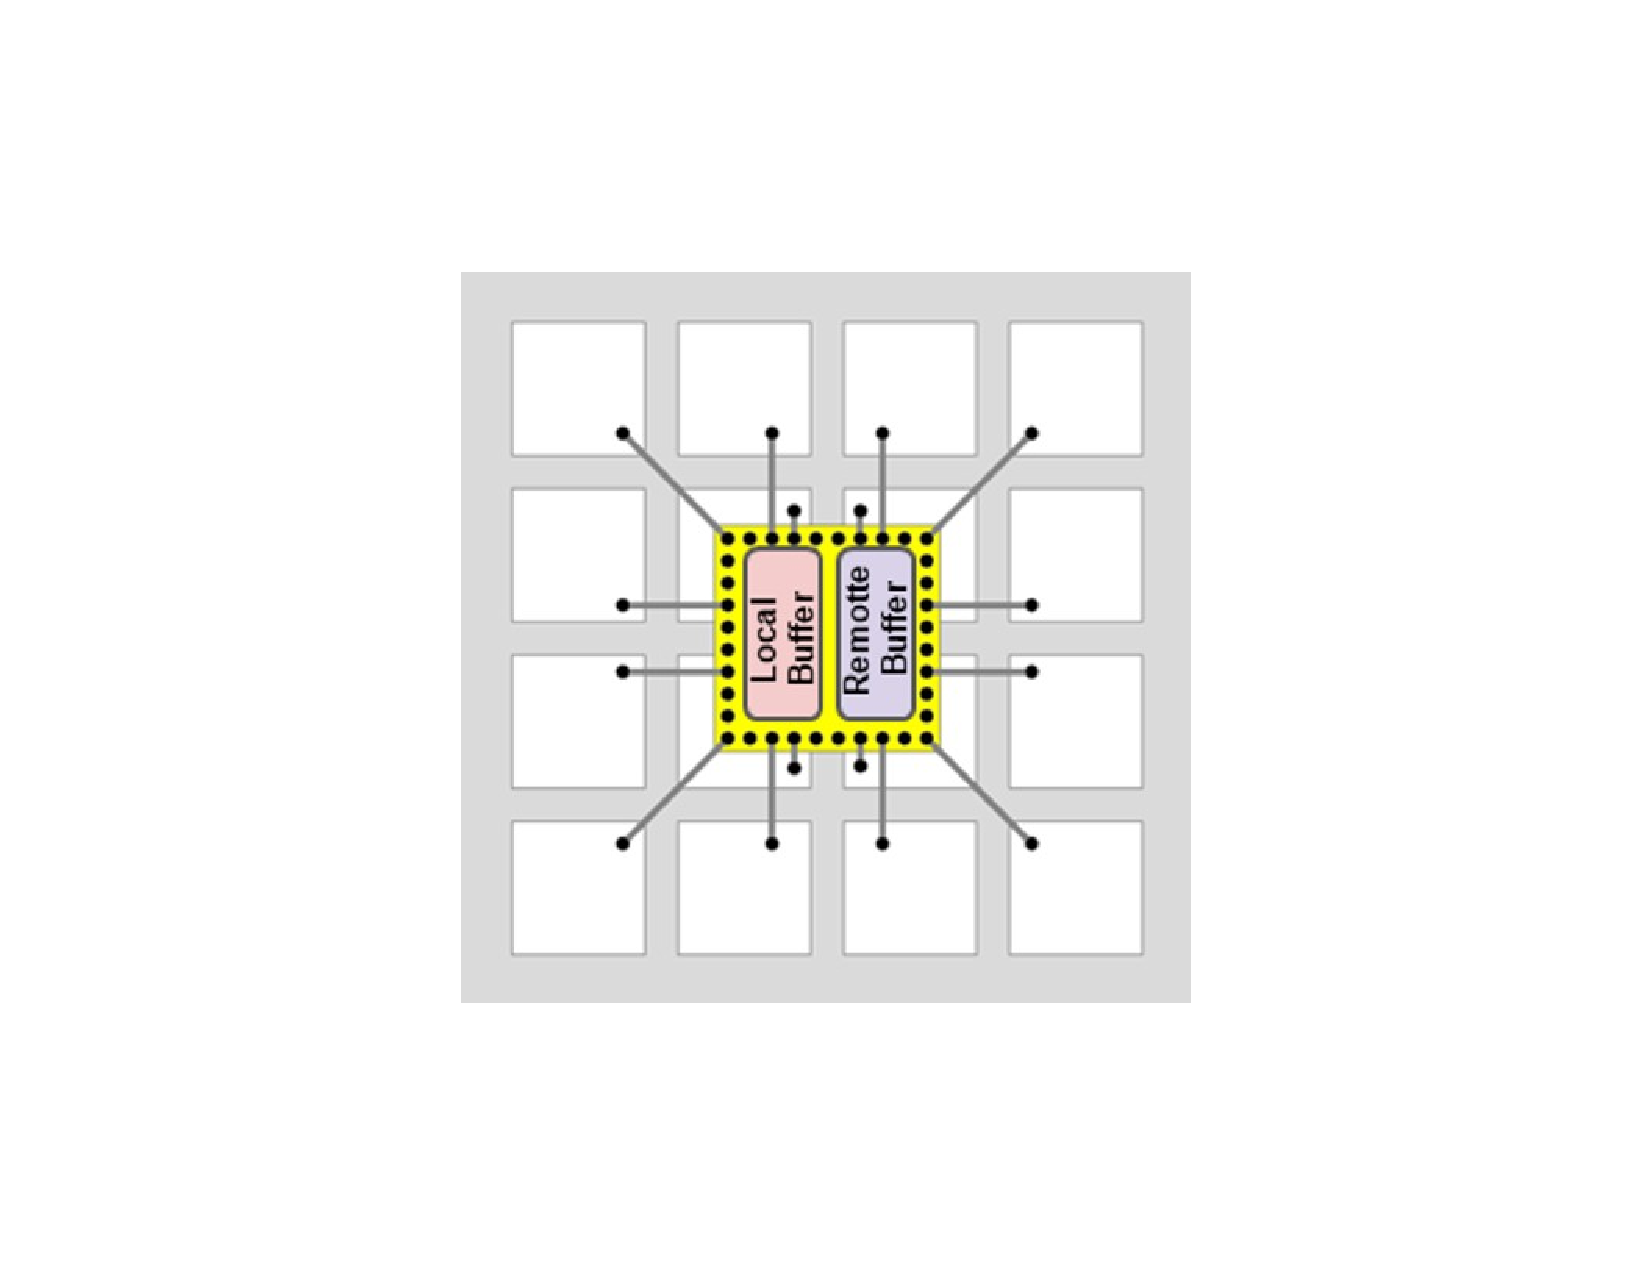
\includegraphics[width=\textwidth]{images/asic_FIFO_image.pdf}
  \caption{Individual node with local and remote FIFOs.}
\end{subfigure}%
\begin{subfigure}{.5\textwidth}
  \centering
  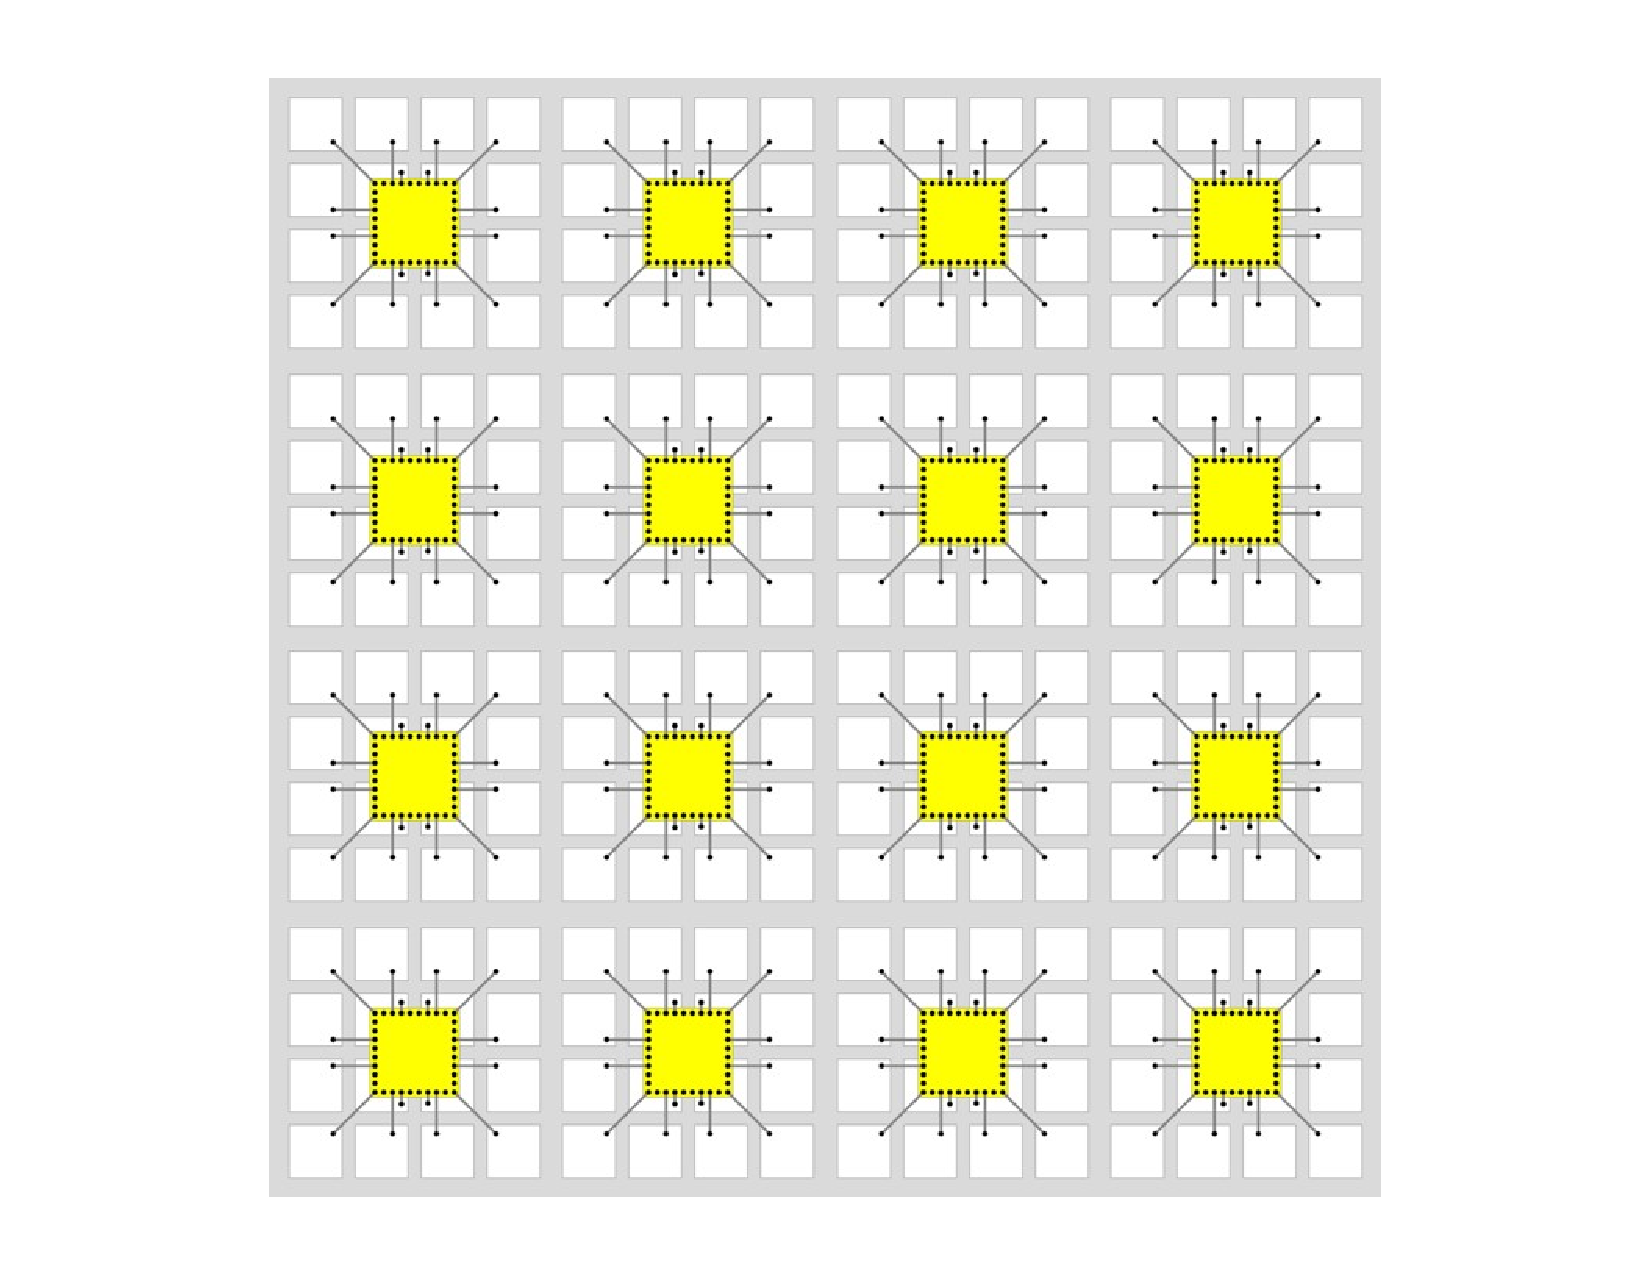
\includegraphics[width=\textwidth]{images/asic_tile_FIFO_image.pdf}
  \caption{Tile of node objects.}
\end{subfigure}
\caption{Composition of an example 4$\times$4 tile.
Each node in the tile represents a digital ASIC which contains two FIFOs.
One FIFO is used to store timestamps from reset data, which we refer to as the local FIFO.
The other FIFO we call the remote FIFO and is used to store all packet transactions from neighbor nodes.
The local FIFO is 48 bits wide, where 32 bits come from the timestamp and 16 bits are from the pixels.
The remote FIFO is 60 bits wide, since it must store all relevant bits for the 64 bit packet word, where there are 4 unused bits.
}
\label{fig:node_fifo_objects}
\end{figure}

There are two types of remote data to send: broadcasts and responses.
A broadcast is a register request sent to a digital node, which can only be created and sent from the aggregator node.
The responses include all other kinds of packets sent from neighbor nodes which include: data packets, event-end packets, and register response packets.

The communication packet object is a custom struct object which uses an enumerated type to differentiate the kinds of packets that the digital node can read from its remote FIFO.
Each simulated node's behavior to these incoming packets is mirrored to the digital FSM, shown in Fig.~\ref{fig:digital_fsm}.
When a node reads the packet from the remote FIFO it reads the enumerated type to determine how to communicate the packet to its neighbors, just as is done in the physical ASIC.

Also tested in these simulations are tiles which are have a "push" architecture.
This architecture changes the condition for a node to leave its idle state and send local data whenever the local FIFO is not empty.
For this reason the push architecture is also more time consuming to simulate since each node can send a packet at any time, provided that it will inject a hit into its local FIFO following the procedure described in the next section.
Nodes which require an interrogation in order to send local data we refer to as the "pull" architecture.

\subsection{Injected Resets}~\label{sec:hits}

In order to speed up the execution of the python simulation reset events are precalculated and loaded into separate list containers for each node.
At the beginning of every simulation time step every node checks its injected resets list against the new simulation step time.
If the new time step is larger than any of the timestamps in its resets list, the resets are then removed from this list and are written to the node's local FIFO.

Resets from simulated data whether radiogenic or neutrino data can occur at any pixel and at any time.
The digital node (and the ASIC) is capable of recording multiple resets from multiple channels at the same time.
This means that it is possible for multiple different pixel resets to only contribute to one local FIFO write.
Therefore, extra care must taken when adding injected resets with channel information.

In this simulation we consider the best case timestamp measurement for each reset, which is that each digital node can record a unique reset for each channel on every new clock cycle. 
Then, procedure for combining resets from multiple channels calculates the clock cycle (timestamp) for which this node would record a timestamp for a particular channel.
If a reset has already been recorded for this channel, the un-injected timestamp is incremented by one clock period for this node.
The above procedure then repeats until all channels have had all of their resets recorded on unique timestamps for the digital node, where only different channels can be recorded on the same timestamp.

\begin{figure}[]
\centering
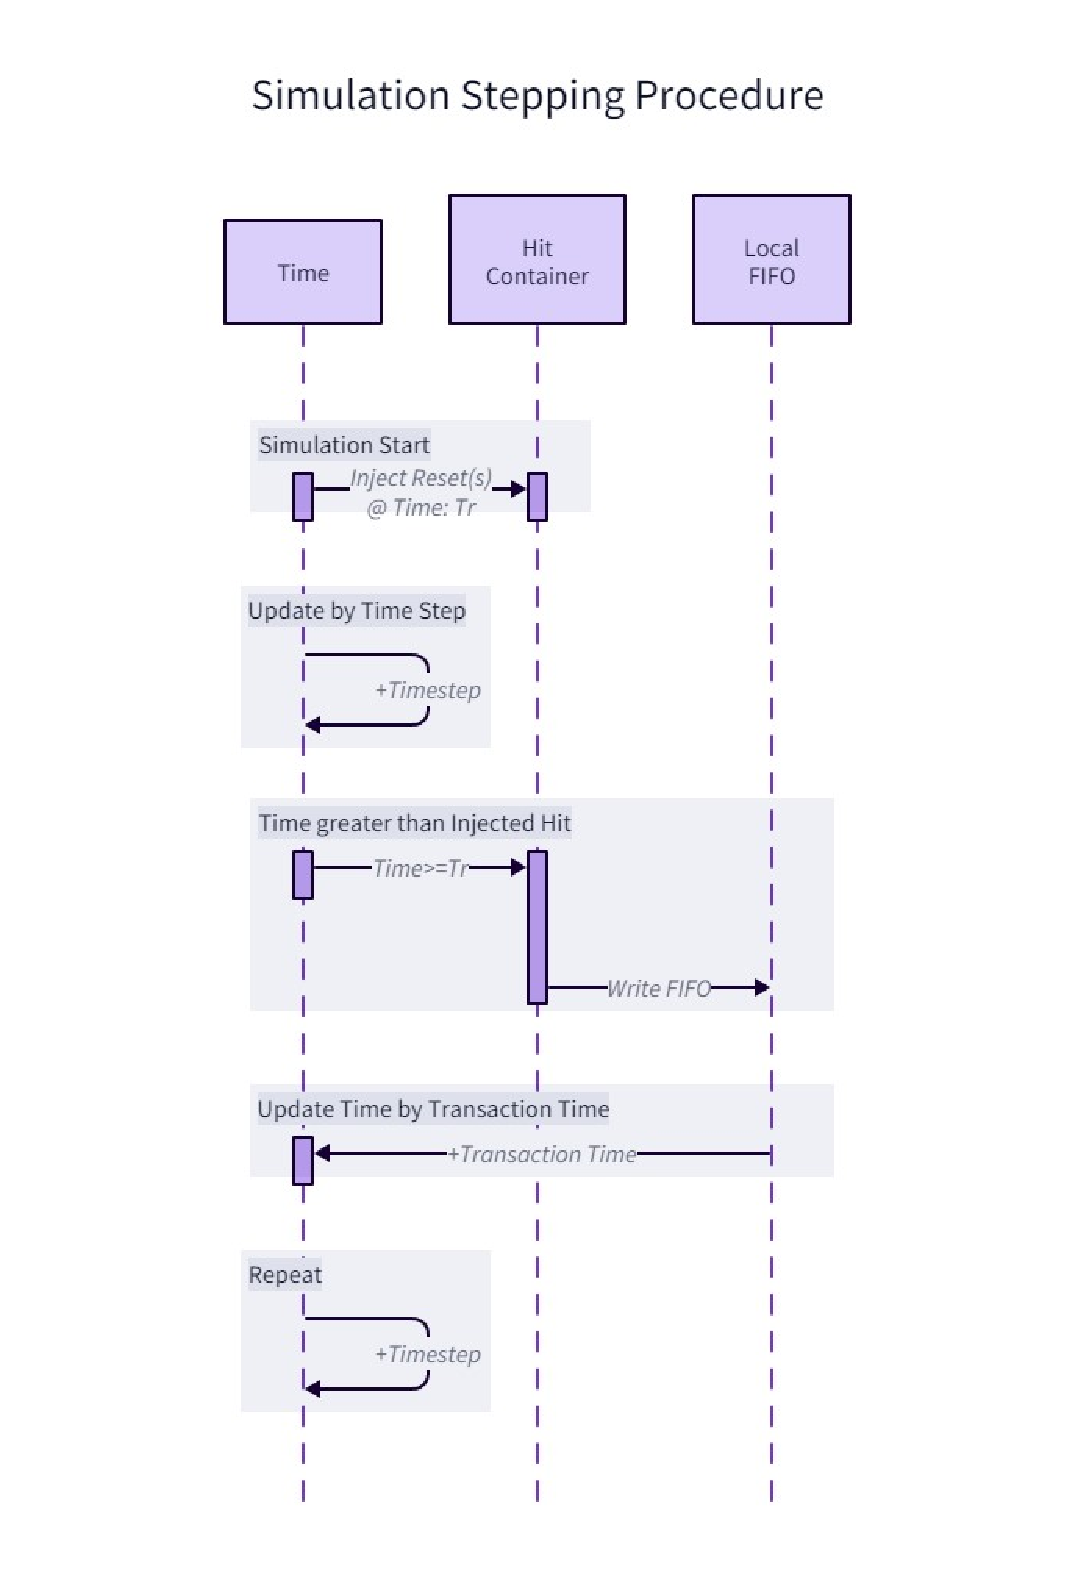
\includegraphics[width=0.7\textwidth]{images/simulation_step_procedure.pdf}
\caption{Example timeline for simulation time steps and injected hits.
Before the simulation begins hits are added into a Hit Container for each node.
When the simulation begins the time is incremented by a single time step ($\tau = 1 \mu$\unit{s}).
The time increments until it is larger than the time of any of the injected hits.
The values of the timestamps are then moved from the Hits container into the local FIFO, where the timestamp that is recorded is the soonest clock cycle after the "true" time of the injected hit.
When the data are ready to be transmitted from the local FIFO, the time is then updated by transaction time.
An example of this procedure is shown in Figure~\ref{fig:push_arch_verification}. 
}
\end{figure}~\label{fig:simulation_step_procedure}

\subsection{The Simulation Procedure}~\label{sec:process}

Upcoming sections will discuss values derived from simulating the readout of the tile. 
Here we briefly describe the simulation procedure and how the results are obtained.
The procedure is also graphically demonstrated in Figure~\ref{fig:simulation_process_procedure}.

The simulation loop iteratively processes a single transaction from a queue of transactions and then processes all nodes in the tile at incremental timestamps.
The timesteps used in the simulation results used here are steps 1~\unit{\mu s}.
It is not necessary to perform smaller time steps than this, as packet transactions themselves are on the order of $\approx 50 \unit{\mu s}$, based on the endeavor protocol.
If any processed node generates a new transaction(s), this transaction(s) is added to the transaction queue.

\begin{figure}[]
\centering
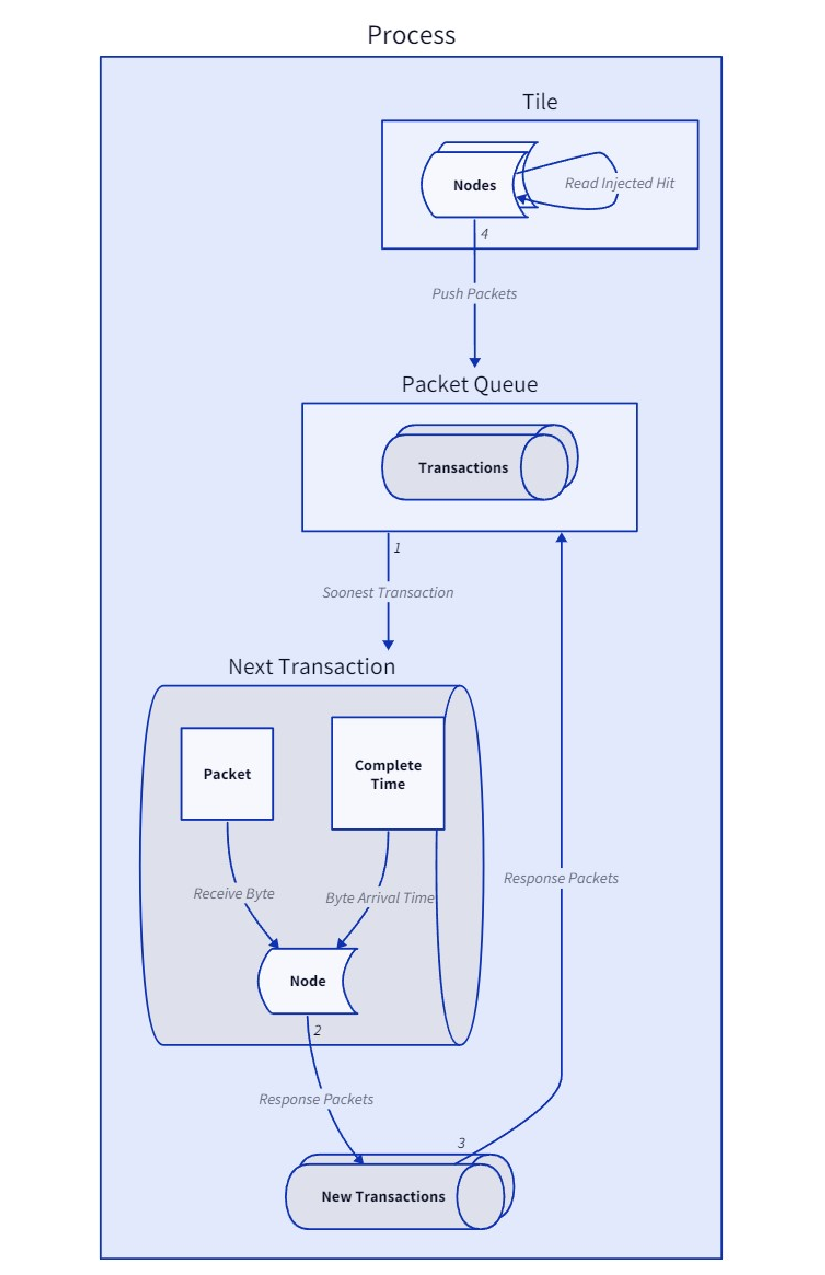
\includegraphics[width=0.65\textwidth]{images/simulation_process_method.pdf}
\caption{Flow chart of the simulation process method which occurs for every simulation time step.
The simulation contains a queue of packet transactions.
The queue is sorted by ascending time, so that the earliest transaction completed time is processed first.
Each transaction contains a packet, a node, and the time the packet arrives.
When the node receives the packet, it can optionally create more transactions, depending on the node's state and the packet.
Any additional transactions are added to the simulation queue, and are time sorted.
The simulation then increments the time for all other nodes within the tile.
This procedure repeats until all nodes in the tile reach the designated time (11~\unit{seconds}).
}
\end{figure}~\label{fig:simulation_process_procedure}

A transaction represents a 64-bit packet that is transferred between two nodes (Sect.~\ref{sec:comms}).
The sending node is responsible for calculating the true time when this transaction would complete.
The receiving node records this byte onto its remote FIFO and performs the state check based on this packet according to Fig~\ref{fig:digital_fsm}.
Then the receiving node updates its time to its soonest clock cycle after this transaction completed.
Next, each node in the entire tile is processed one forward timestep.
If nodes are in the push state and receive a hit within this timestep window, they create a new outgoing packet, and add this packet to the transaction queue.
We note that it is only possible for processed nodes which did not receive the transaction packet to create a new packet if they are in a push-based architecture. 

The simulation is complete when all nodes have been processed up to the final requested time and no transactions are left in the queue. 
In the results presented here we process the tile for one second longer than any injected resets to ensure that the tile is fully read out.


\section{The Tile Parameters}

One goal of the simulations presented here is to parameterize different design choices in constructing both the digital nodes and the tiles.
The different parameters which we test are described in Table~\ref{table:tile_params}.

There are a total of four parameters to test: frequency stability, tile size, routing, and architecture.
Of the four parameters, we note that the frequency stability is the one parameter determined by the ASIC's physical design.
Therefore, special care must be taken into account when designing the local oscillator for the ASIC.
The other variables: routing, architecture, and tile size are either programmable registers or easily configurable in hardware layout.

It is intuitive (and the results indicate) that improved frequency stability leads to a more stable design.
Nevertheless, we find it enlightening to demonstrate how remote buffer depths are affected in the case of a 5\% (0.5\%) clock deviation.
When a tile is created with 5\% (0.5\%) frequency deviation each node within the tile is created by randomly sampling from a Gaussian distribution with a mean of 30$\unit{MHz}$ and a standard deviation of 5\% (0.5\%).
Since many ($\approx 10^4$) events are performed per tile configuration each tile is created with a random seed to ensure that each node is created with the same frequency for each test.

\begin{table}
\begin{center}
\begin{tabular}{|| p{30mm} | p{30mm} | p{90mm} ||}
 \hline
 Parameter & Values Taken & Description \\ [0.5ex]
 \hline\hline
  Oscillator\newline Frequency & 0.5\%, 5\% & High variance causes packet buildup or drift within the tile depending on whether packets are sent from slow to fast, or fast to slow clocks. \\
 \hline
  Tile Size & 4$\times$4, 8$\times$8\newline 10$\times$14, 16$\times$16 & Affects total number of resets which must be routed to aggregator.\\
 \hline
  Routing & Snake, Left, and Trunk & Tiles with different routing are effectively different graphs which affect packet buildup~(\ref{eq:adjacency_matr}). Different combinations of edges between nodes can cause packet buildup if nodes have more input edges than output edges.  \\
 \hline
  Architecture & Push, Pull & Describes conditions for when node enters transmit-local state.~\ref{sec:local_data_packet}. The push architecture allows individual nodes to transmit data when data are received, whereas pull architecture only send data upon receiving a special request packet from the aggregator.  \\
 \hline
\end{tabular}
\caption{The different tile parameters that are used for the effective tile search.
  The frequency drift relates the relative distribution of the frequency of adjacent oscillators.
  The tile size determines how many digital nodes are within a single tile.
  The routing configurations are described in detail in the previous chapter, and refer to how local data words are sent to the aggregator.
  The two different architectures define how the node enters the transmit local state.
  The push architecture enters whenever a new reset is acquired, whereas the pull architecture enters only when a data request is received from the aggregator.}
\label{table:tile_params}
\end{center}
\end{table}

The other design parameters are readily configurable in either hardware (tile size) or through register configurations of the digital node (routing and, possibly, architecture).
Tile size is mostly an engineering and cost constraint.
Larger tile sizes mean the full design would require less aggregator nodes and require less tiles to parameterize.
We show results for small tile sizes to indicate possible connections portions of larger tiles could configure.
The largest tile size we tested was 16 $\times$ 16 as the current limit in the Q-Pix digital prototype only allocates four bits for each x or y coordinate in a tile.

The routing and architecture parameters help guide the digital design efforts design of the digital ASIC.
In practice it is all but certain that implemented routing for a digital tile will take on a combination of the routing styles described here.
The reason for this is simply that is likely that some digital nodes will fail (for whatever reason) in the life time of a DUNE-FD 10 kT module.
Therefore, future tiles that contain hybrid routing we suggest to those users to individually analyze the sub tiles with appropriating routing and frequency distribution and determine if the buffer depths are appropriate.

\subsection{Oscillator Frequency and Drift}

Two different oscillator frequencies are tested, as shown in Table~\ref{table:tile_params}.
These different frequency variances indicate mean differences in oscillator frequency between adjacent nodes.
An example of the 5\% oscillator variance is shown in Figure~\ref{fig:asic_frequency_example}.
The values plotted in this figure indicate relative factors above or below the expected 30\unit{MHz} mean.

Local oscillator drift was not included as a testing parameter since transactions occur over small time scales compared to any likely meaningful oscillator drift.
If these drifts occur on time scales much longer than the interrogation time than the oscillator, the frequency could be continually re-calculated with the method shown in the previous chapter.
If these drifts are periodic about a mean frequency and on time scales much smaller than the interrogation time window then the drifts would average out.
In the event that clock drift timescales are on the interrogation timescale ($\approx 1\unit{s}$), then this is equivalent to a frequency uncertainty for the entire transaction cycle.
This would mean that an oscillator has a $\approx 5\%$ uncertainty in its frequency on each interrogation.
Such a node would not be able to reconstruct timestamps, and therefore not be able to reconstruct the z-position of charge with the required 1$\unit{ppm}$ estimated uncertainty for Q-Pix clocks~\citep{qpix:nygren:mei}.

\begin{figure}[]
\centering
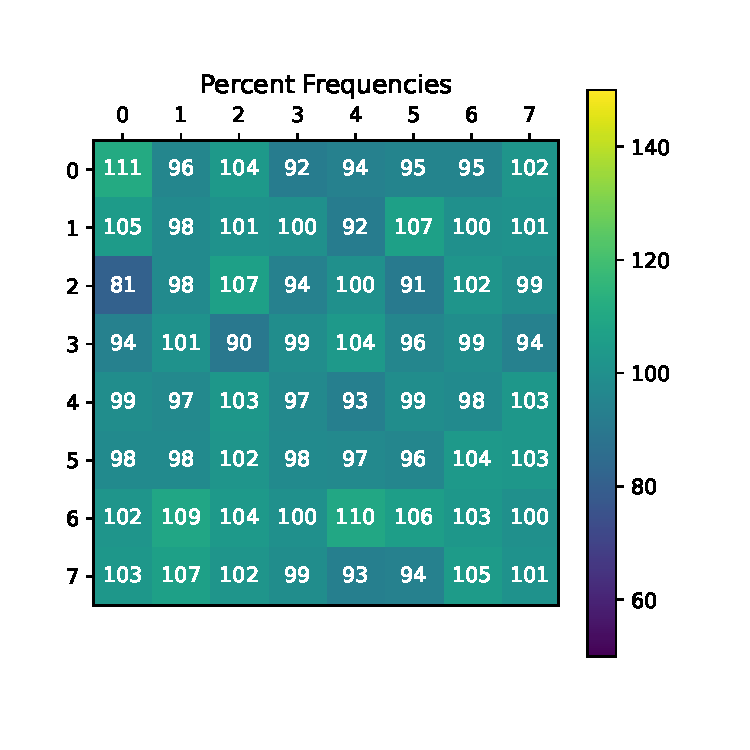
\includegraphics[width=\textwidth]{images/asic_frequency.pdf}
\caption{Distribution of ASIC frequencies used in the 8$\times$8 tile, and in the example FIFO buffer depths for this chapter.
The numbers plotted above each ASIC row and column indicate the relative frequency of this ASIC compared to the nominal 30$\unit{MHz}$ mean.
For example, a number of 112 indicates an ASIC which is 12\% faster than 30MHz, a frequency of $\approx 33.6 MHz$.}
\end{figure}~\label{fig:asic_frequency_example}

\section{Simulating The Tile Readout}~\label{sec:simulating_tile}

The tile simulation is performed by injecting hits from two known sources: radiogenic backgrounds and beam neutrinos.
All results presented in this chapter are based on 11 seconds of simulated run time.
Radiogenic data are collected and used to occupy 10 seconds of background noise resets.
The higher intensity neutrino events are offset so that interaction occurs at $t = 5.1 s$.
The simulation is run for a total of 11 seconds, instead of 10, to ensure that all of the packets are collected by the aggregator node.
In practice, there would be additional resets from backgrounds which occur in that final second of data.
However, the number of resets from the radiogenic events are much smaller (by about two orders of magnitude) than the neutrino events.

The full readout of the tile occurs based on the number of packets times the average transaction length.
$$
T_{readout} \approx 50 \mu s \times N_{max packets}
$$

If we set $T_{readout}$ to 1 second:
$$
N_{max packets} \approx  20000
$$

Since the simulation is run six seconds longer than the origin time of the neutrino events all reset events are be accounted for if neutrino events cause less than $\approx 120000$ resets.
There are no simulated neutrino events which create these number of resets since this would require an energy of $\approx$ 15\unit{GeV} deposited into the LAr.

The configuration of each node and the tile happens before the beginning of the simulation.
The frequency and the routing directions are configured for each node during its creation.

\subsection{Simulation Timing}

The purpose of the simulation is the examine the communication behavior of digital nodes at different frequencies which communicate via packets of variable time width.
For this reason special care is taken to ensure that the timing of packet transactions in the simulation are accurate.
The behavior of each node is determined by its state machine properties, as described in Fig.~\ref{fig:digital_fsm}.
Therefore, an accurate measure of timing for each node is equivalent to ensuring that timing of ASIC state transitions are accurate.

%% example snake route
\begin{figure}[]
\centering
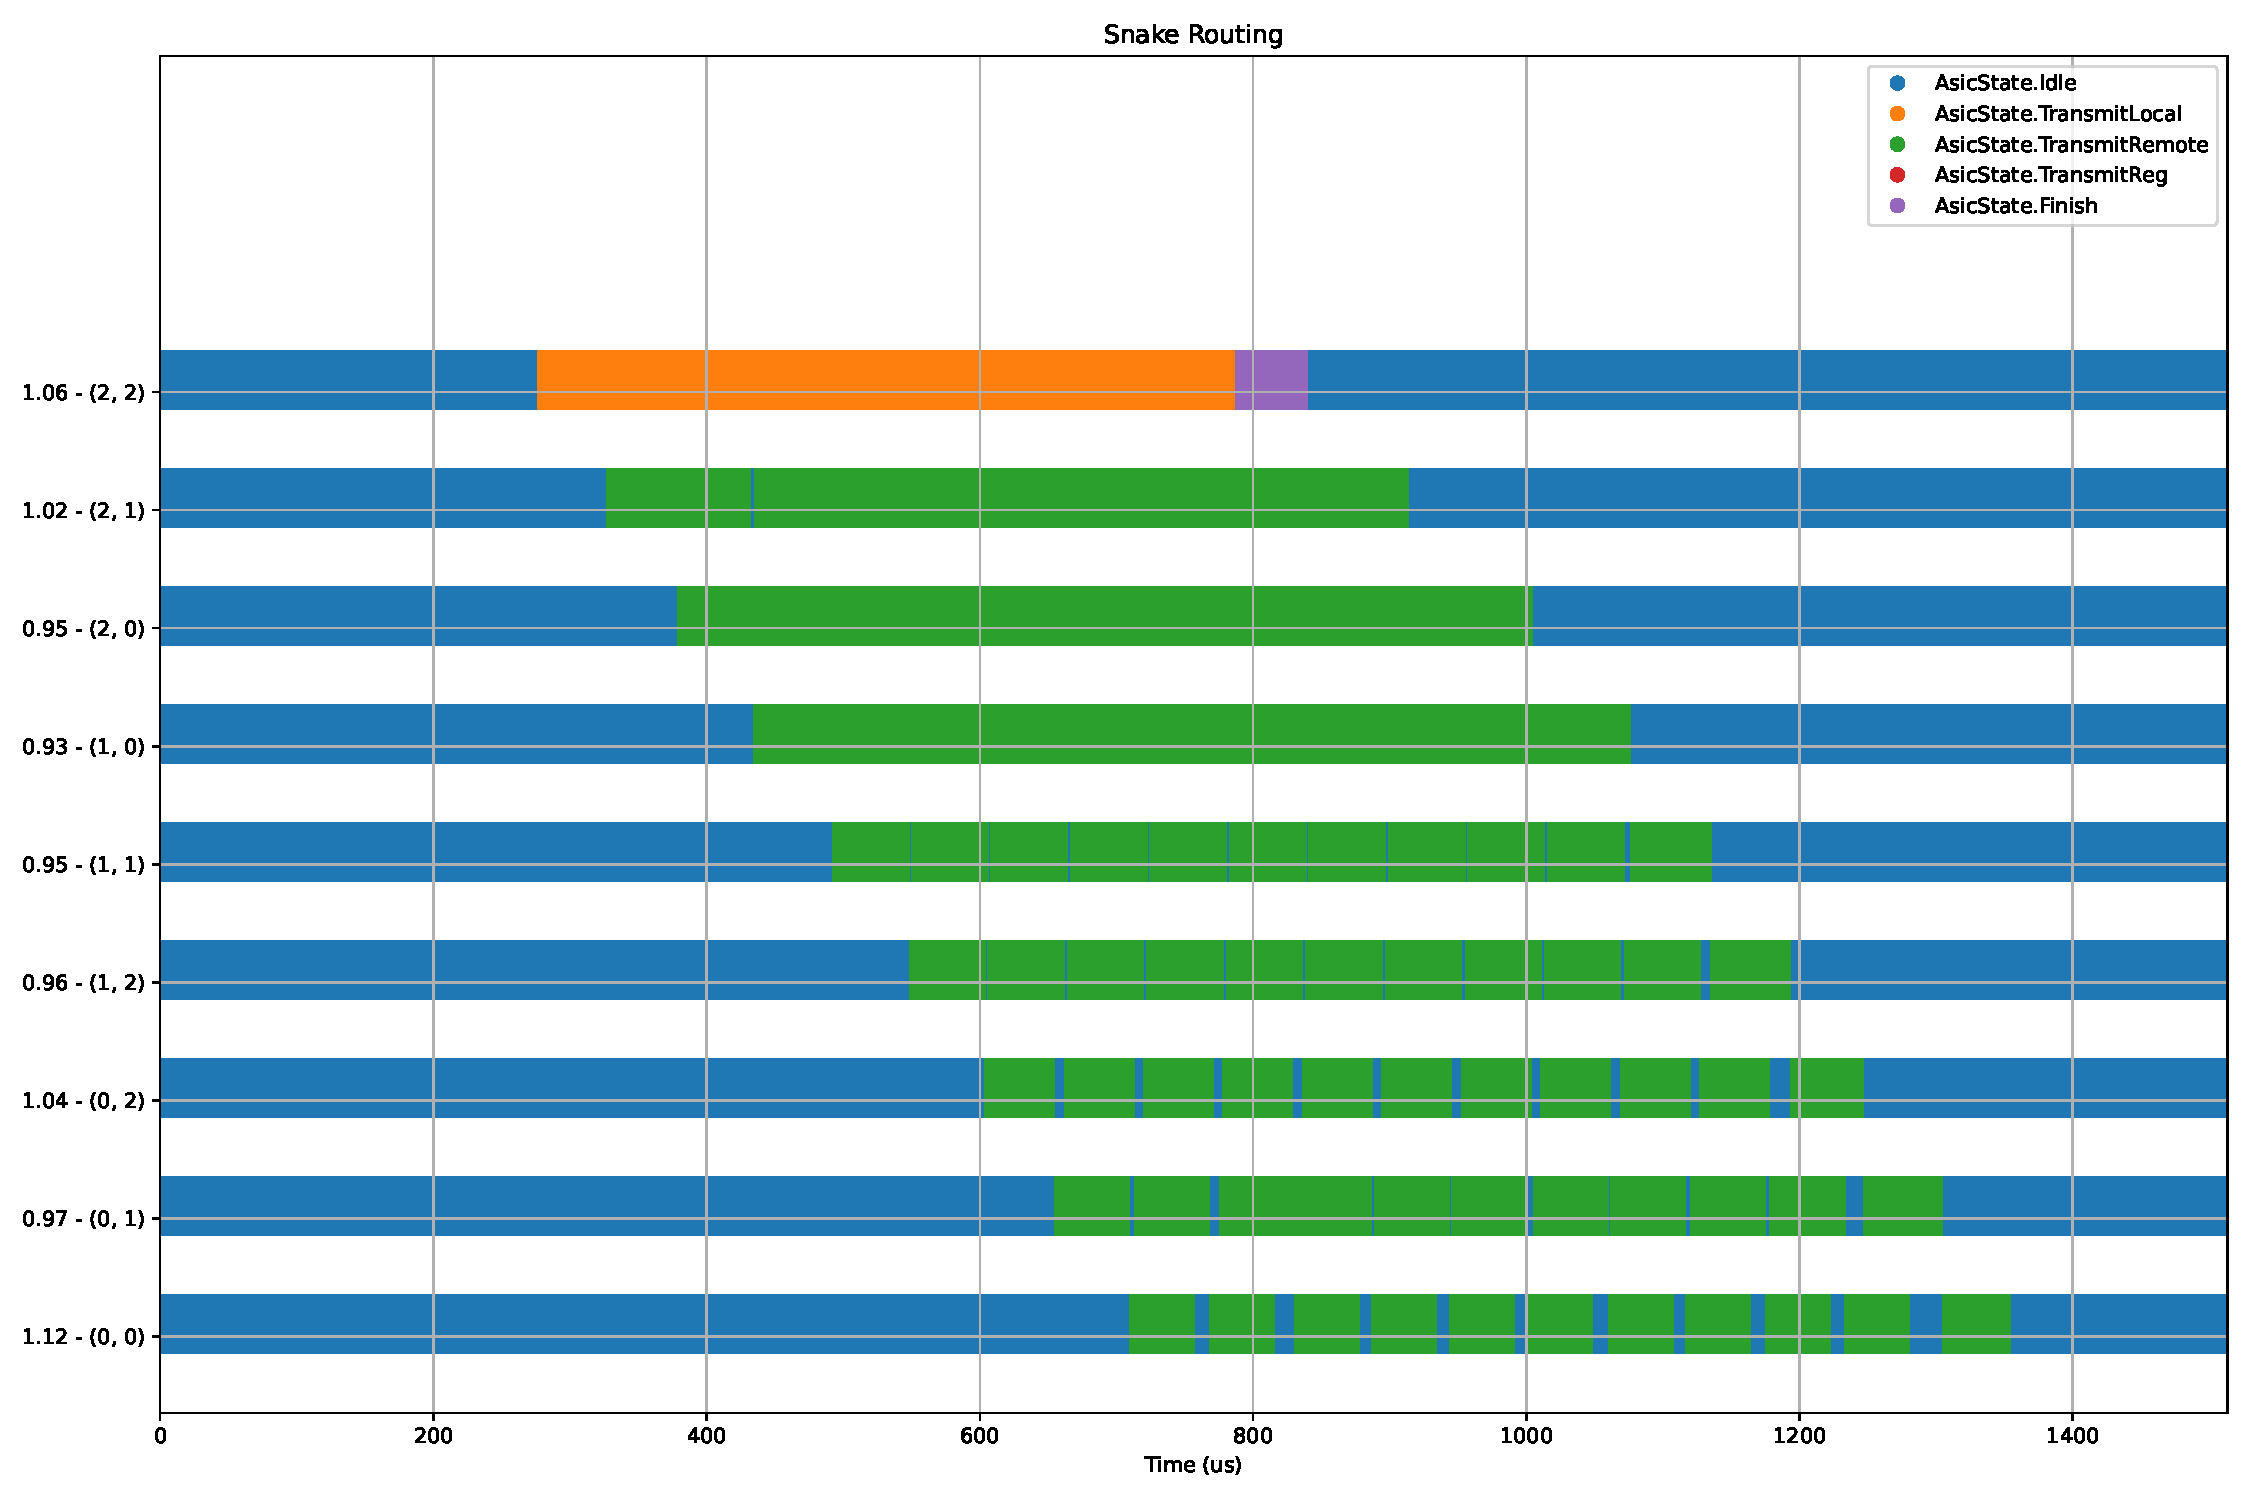
\includegraphics[width=\textwidth]{images/snake_timer.pdf}
\caption{Example of timing ASIC state transitions in the simulation framework.
  The x-axis represents time in $\mu s$, and the different y-axis labels represent different ASICs within a 3$\times$3 tile shown.
  The y-axis also indicates the relative frequencies of the ASICs in the tile, where the node at (0,0) has the fastest frequency, which is 12\% faster than 30 MHz.
  The blue regions indicate that the ASIC is in the idle state.
  The first orange state indicates that this ASIC (2,2) received a register request from the aggregator node and is now sending its local data, concluding in the purple state, which is sending the event end word.
  The Packets drift apart in time as they are sent from slower to faster ASICs.
  Shown here is the possibility of packet drift due to asynchronous packet transfers that depends on the magnitude of the frequency drift between neighbor ASICs.
}
\end{figure}~\label{fig:snake_packet_drift}

Not shown are times when an ASIC receives or responds to a broadcast.
Broadcast packets are uniquely handled by ASICs.
An ASIC, instead of writing the request to the remote FIFO, immediately handles a broadcast by sending this packet to all neighbor ASICs, excluding the direction from which it received the broadcast.
This means that an ASICs state does not change during a broadcast.
This is handled by the simulation by tracking packet times on the ASIC connections.
The broadcast packet is sent starting at the soonest available time on each connection.
The full broadcast procedure is described in Section~\ref{sec:broadcast}.


\subsubsection{Snake Timing Example}~\label{sec:snake_timing}

Here we refer to the "snake" routing as the maximal path routing.
This routing is one that minimizes the number of input edges for all nodes within a tile.
An example of a packet transfer which uses this routing is shown in Figure~\ref{fig:snake_packet_drift}.

Since the snake routing minimizes the number of edges, it also maximizes the number of ASICs responsible for sending remote data in the tile.
This increases the number of remote transactions in a tile readout.
This demonstrated by the amount of time ASICs are in the transmit remote state shown in Figure~\ref{fig:snake_packet_drift}.

%% example local vs remote of snake
\begin{figure}
\centering
\begin{subfigure}{.5\textwidth}
  \centering
  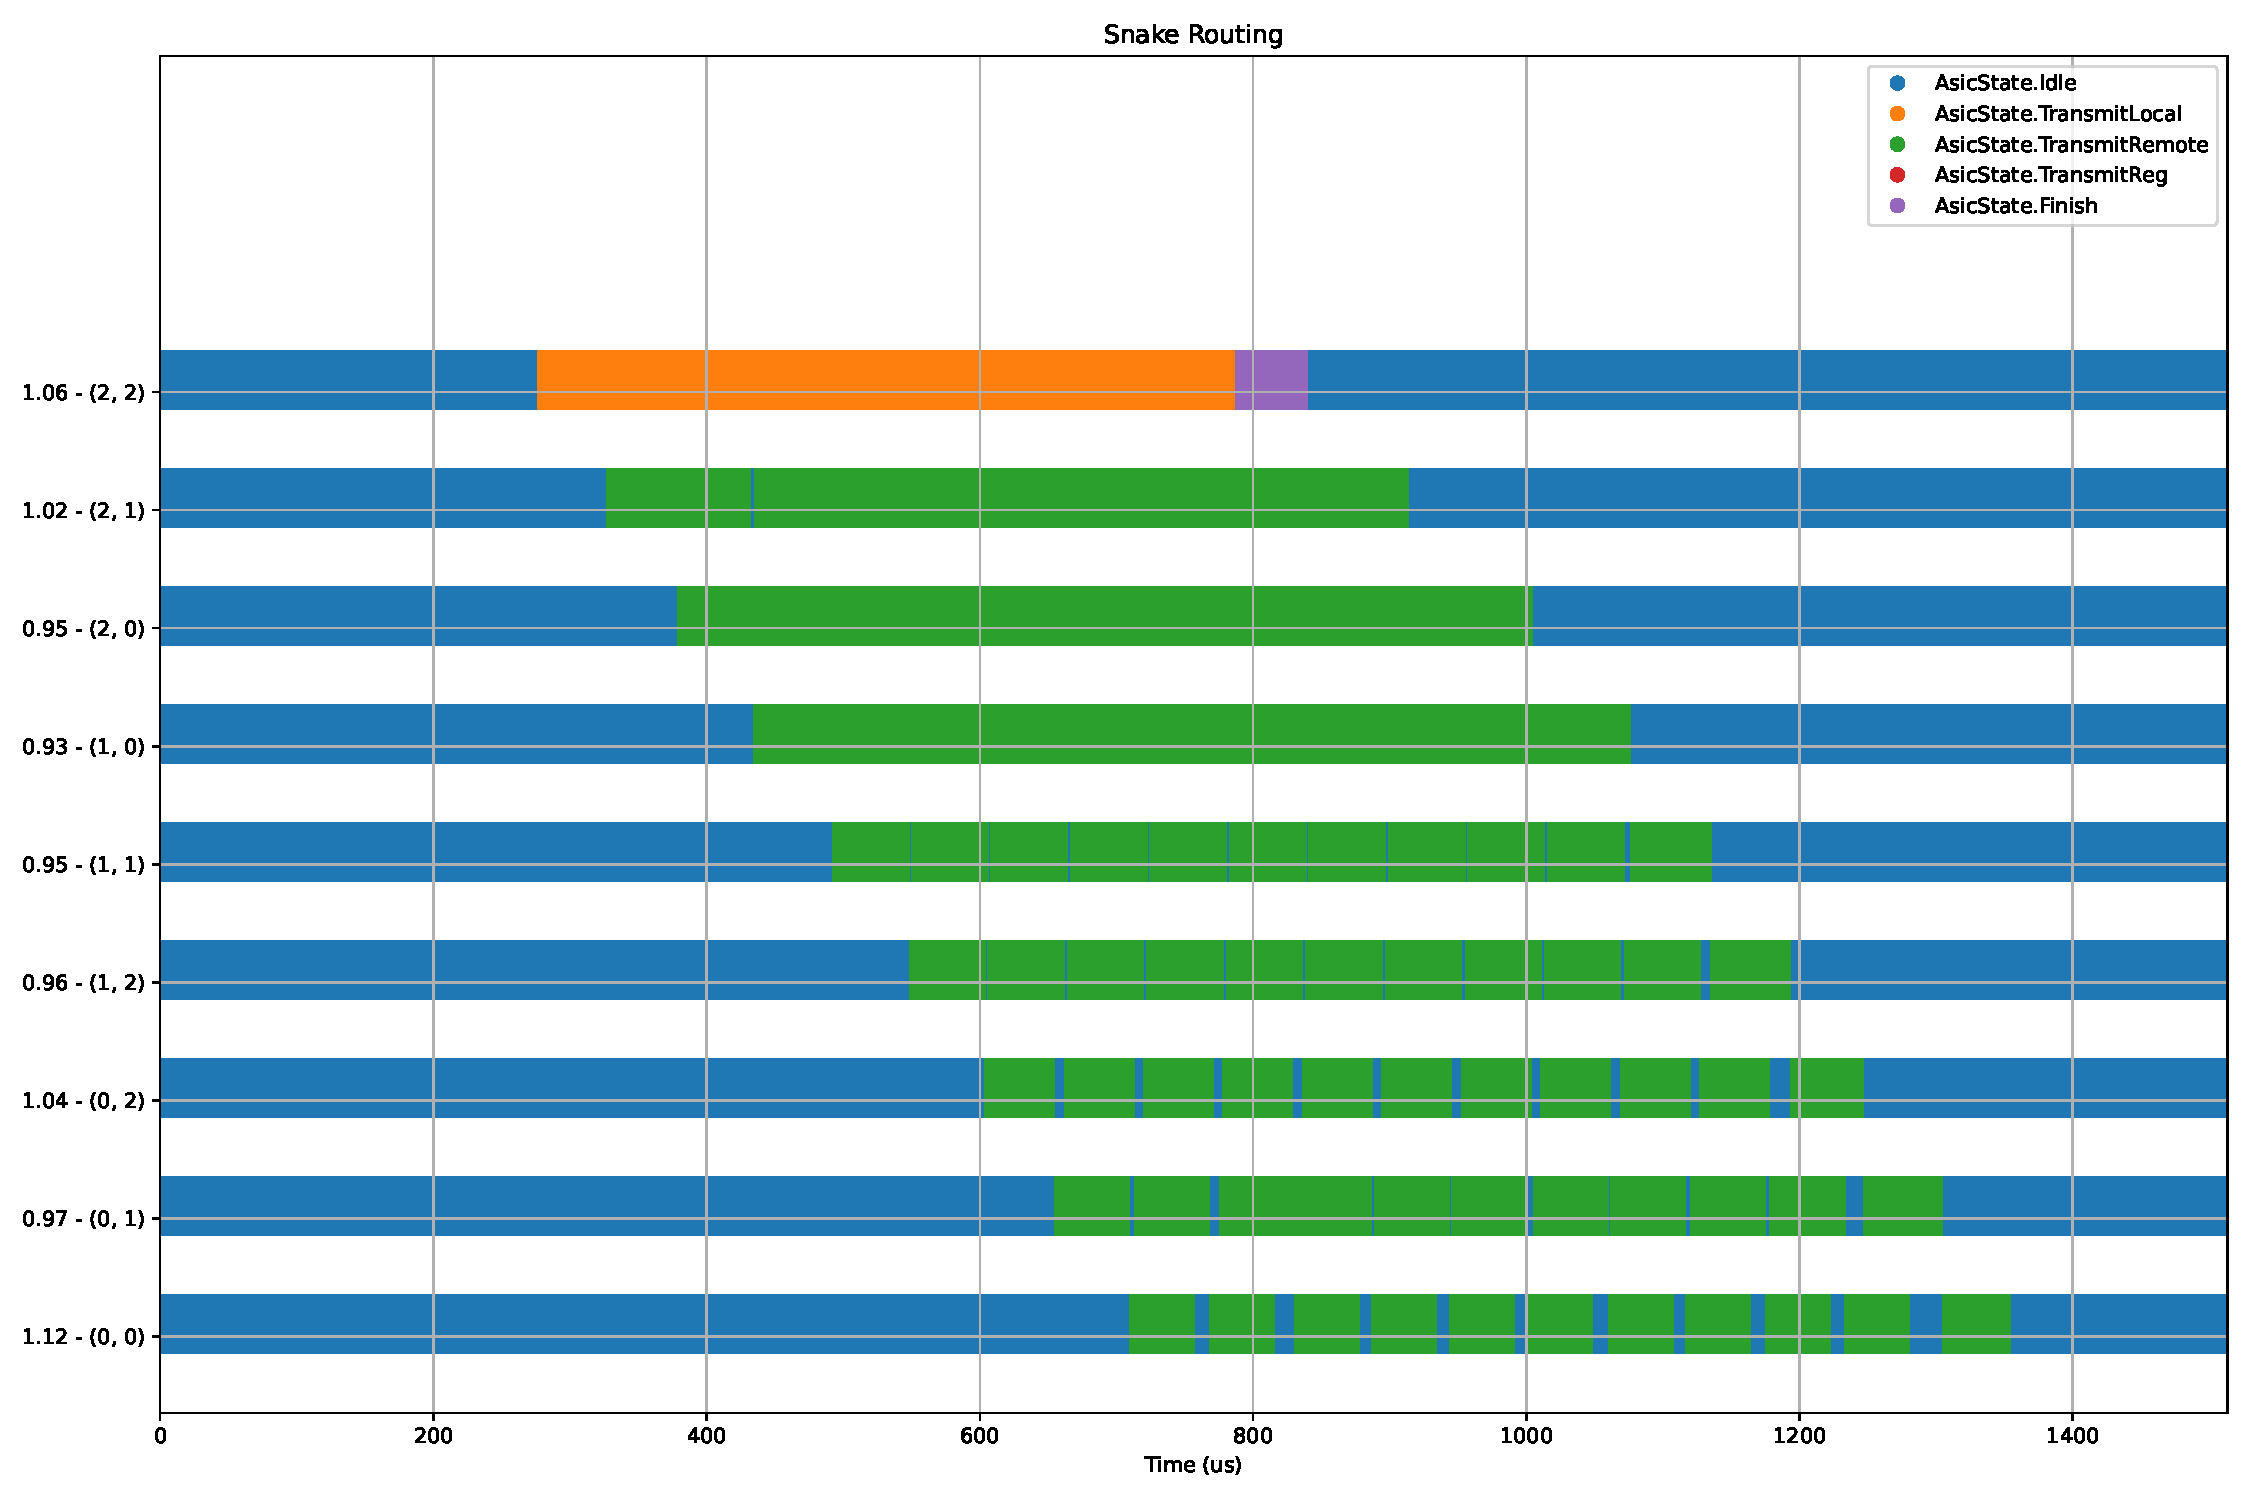
\includegraphics[width=\textwidth]{images/snake_timer.pdf}
  \caption{Snake Readout timing Diagram}
\end{subfigure}%
\begin{subfigure}{.5\textwidth}
  \centering
  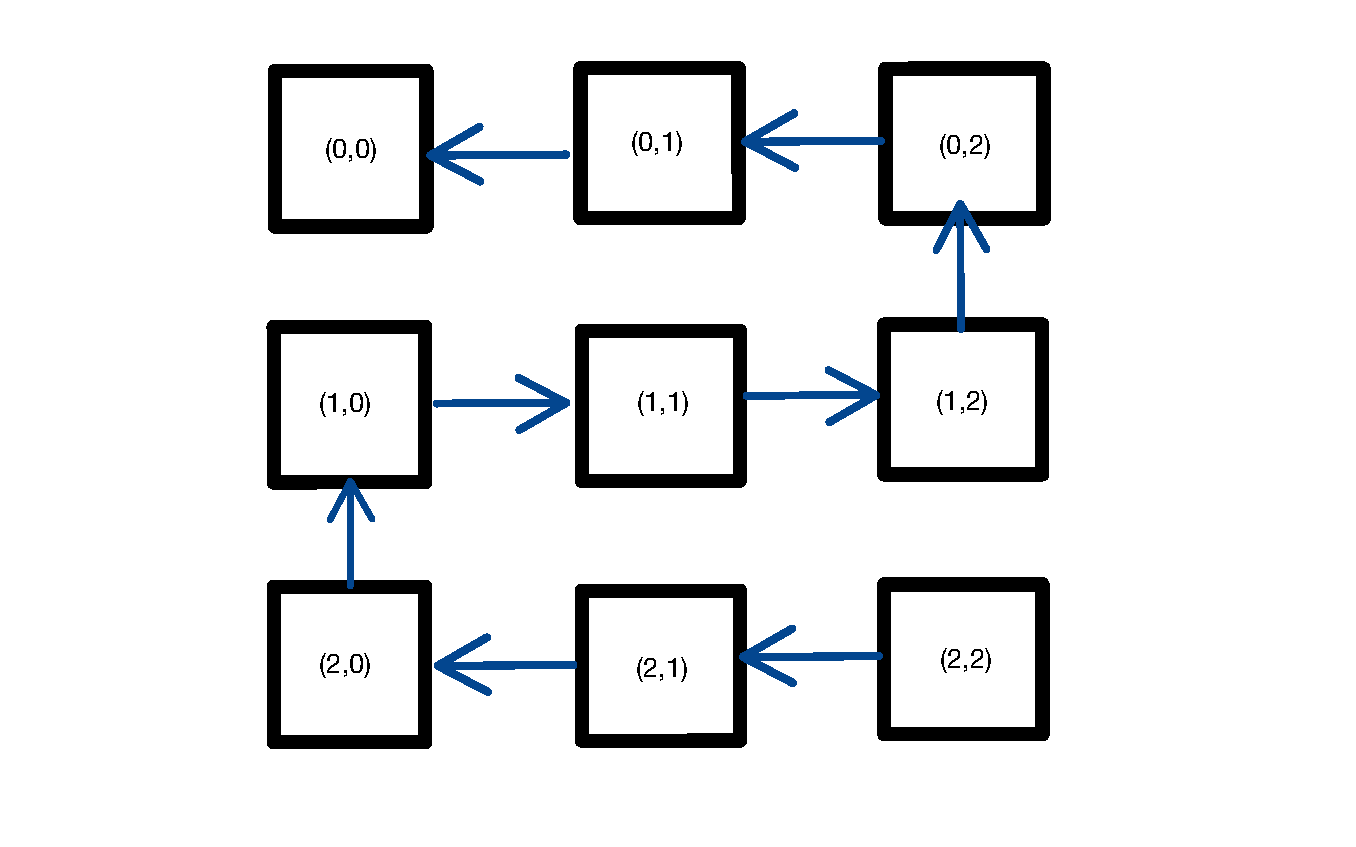
\includegraphics[width=\textwidth]{images/snake_ex_read.pdf}
  \caption{Data Path in Snake Readout}
\end{subfigure}
\caption{A snake packet transaction example is shown. The broadcast is received by the further node (2,2) and 10 data words are sent, followed by a event end word.
Each packet traverses through all nodes in the tile where remote packets are sent immediately.}
\label{fig:snake_timer}
\end{figure}

%% example left route
\subsubsection{Left Timing Example}

The naming convention for the "left" routing is arbitrary since the tile can be viewed from the opposite direction and the routing would appear "right".
By "left" routing we mean a routing configuration in which the routed direction for all ASICs in all rows are in the same direction, except for the nodes which have no neighbor in that direction.
These nodes then are routed "up" towards the aggregator.
An example of a packet transfer with this routing configuration is shown in Figure~\ref{fig:left_packet_drift}.

This routing configuration minimizes the path length for all nodes in the tile when the base-node is at the corner.

\begin{figure}
\centering
\begin{subfigure}{.5\textwidth}
  \centering
  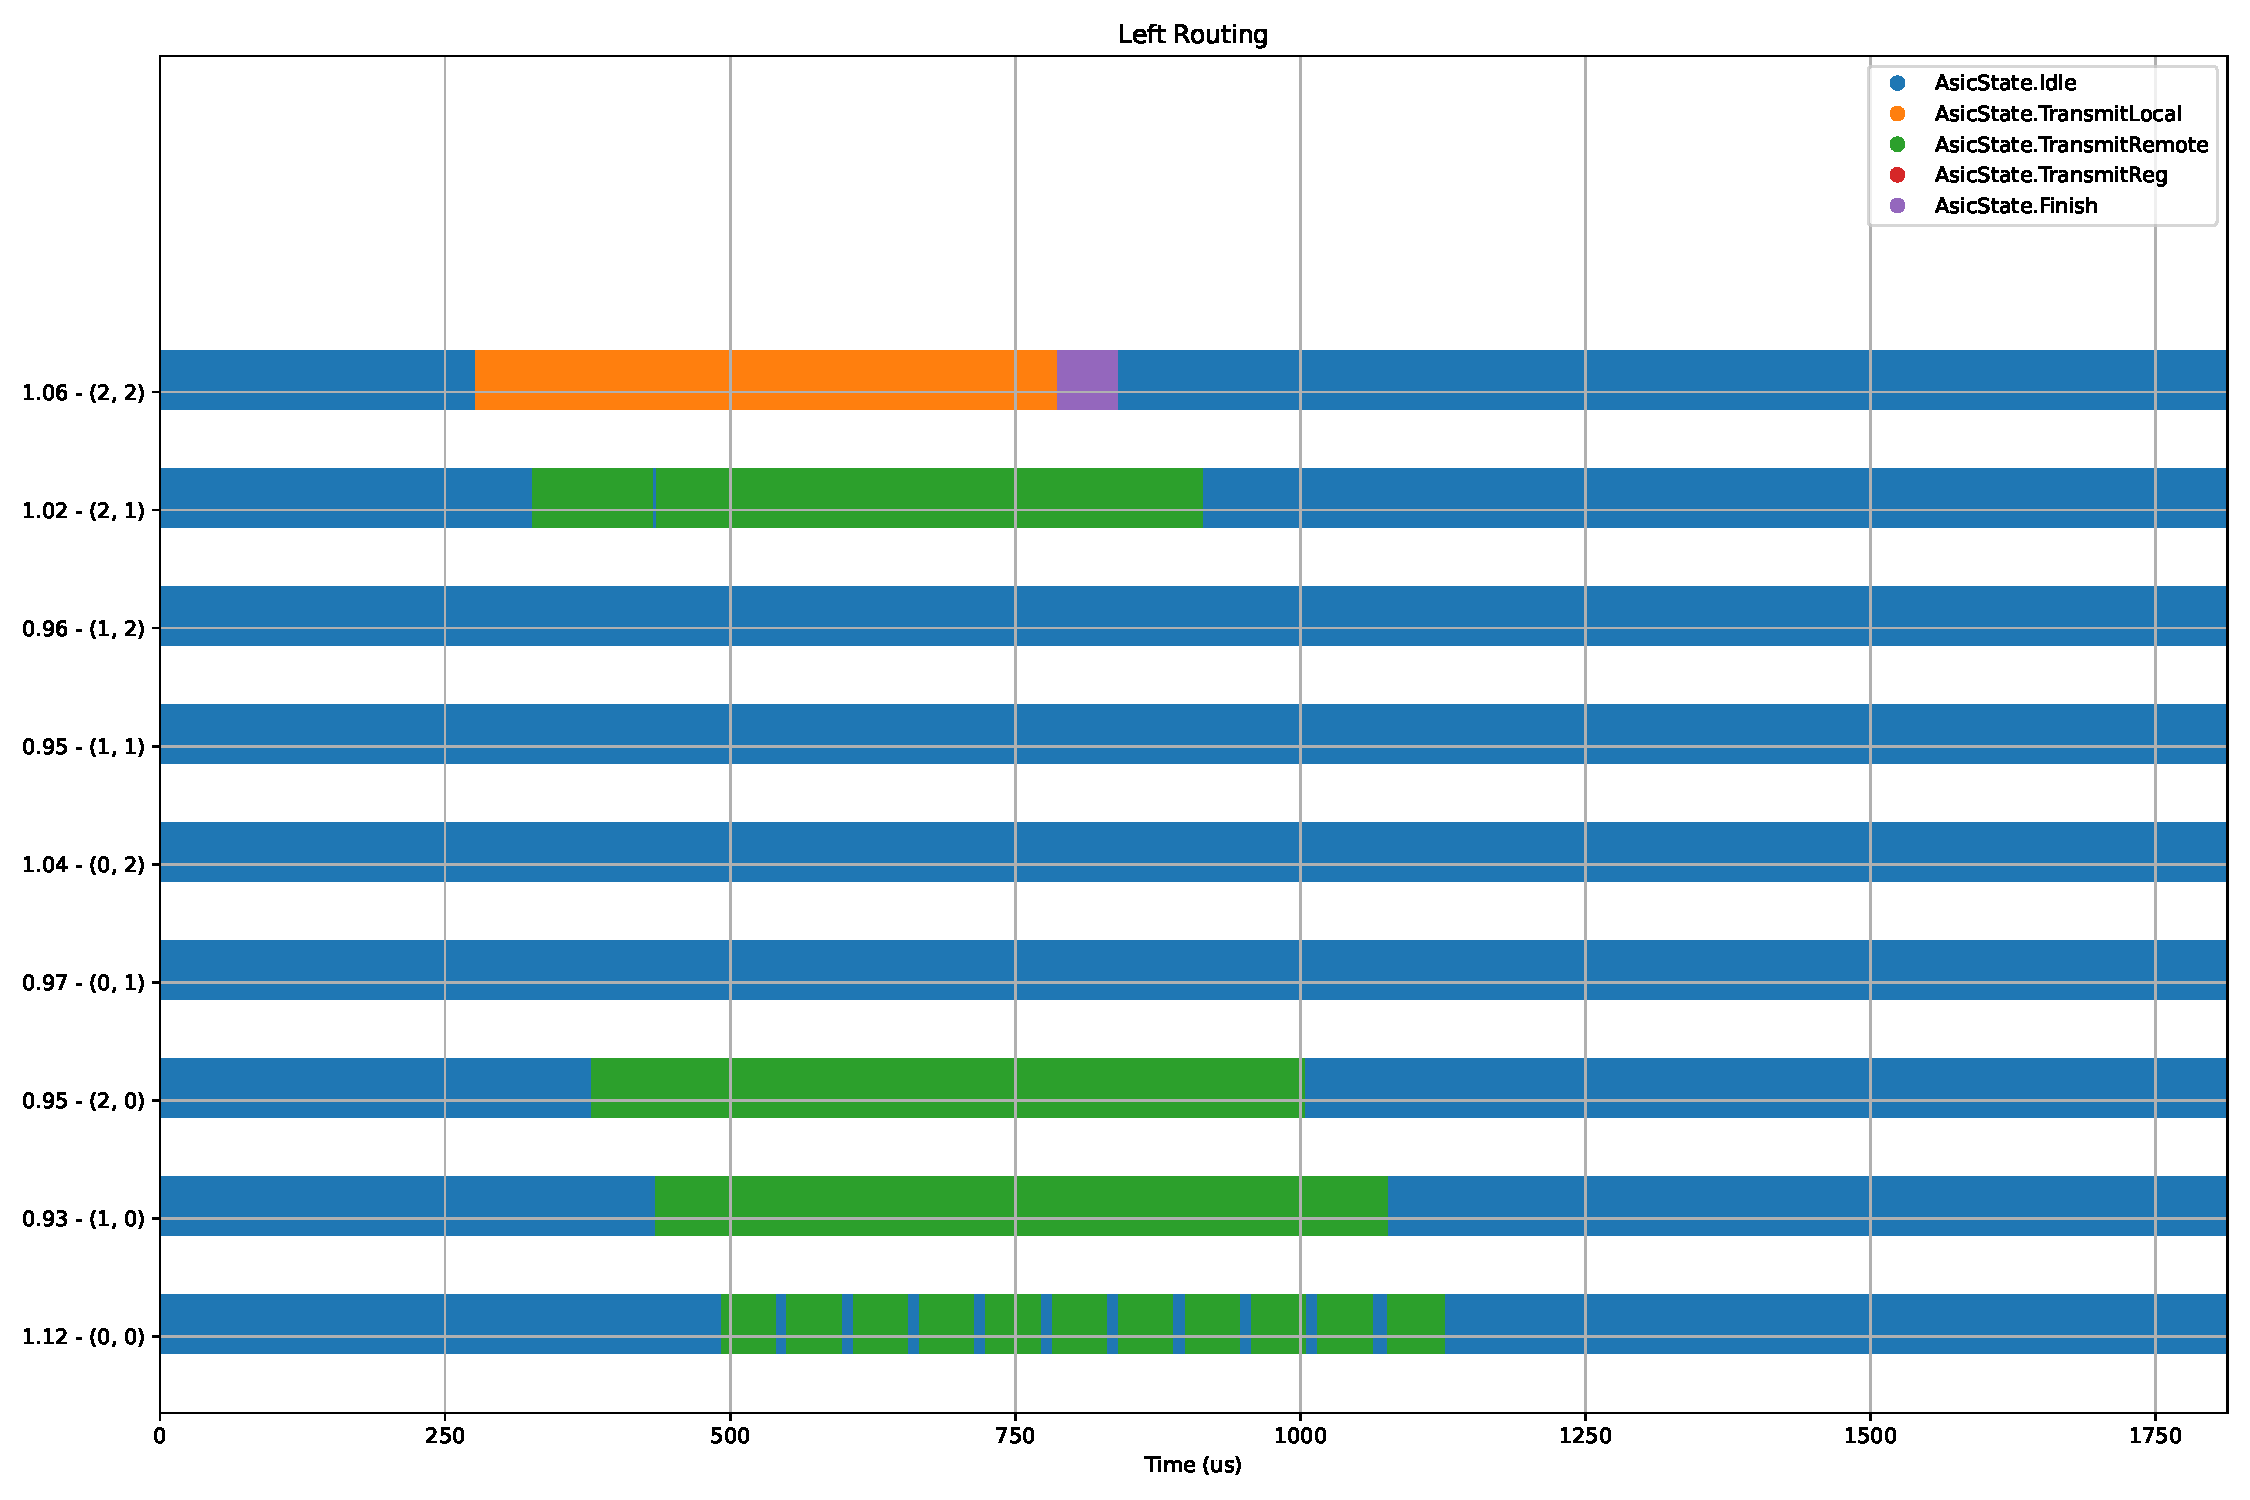
\includegraphics[width=\textwidth]{images/left_timer.pdf}
  \caption{Left Readout timing Diagram}
\end{subfigure}%
\begin{subfigure}{.5\textwidth}
  \centering
  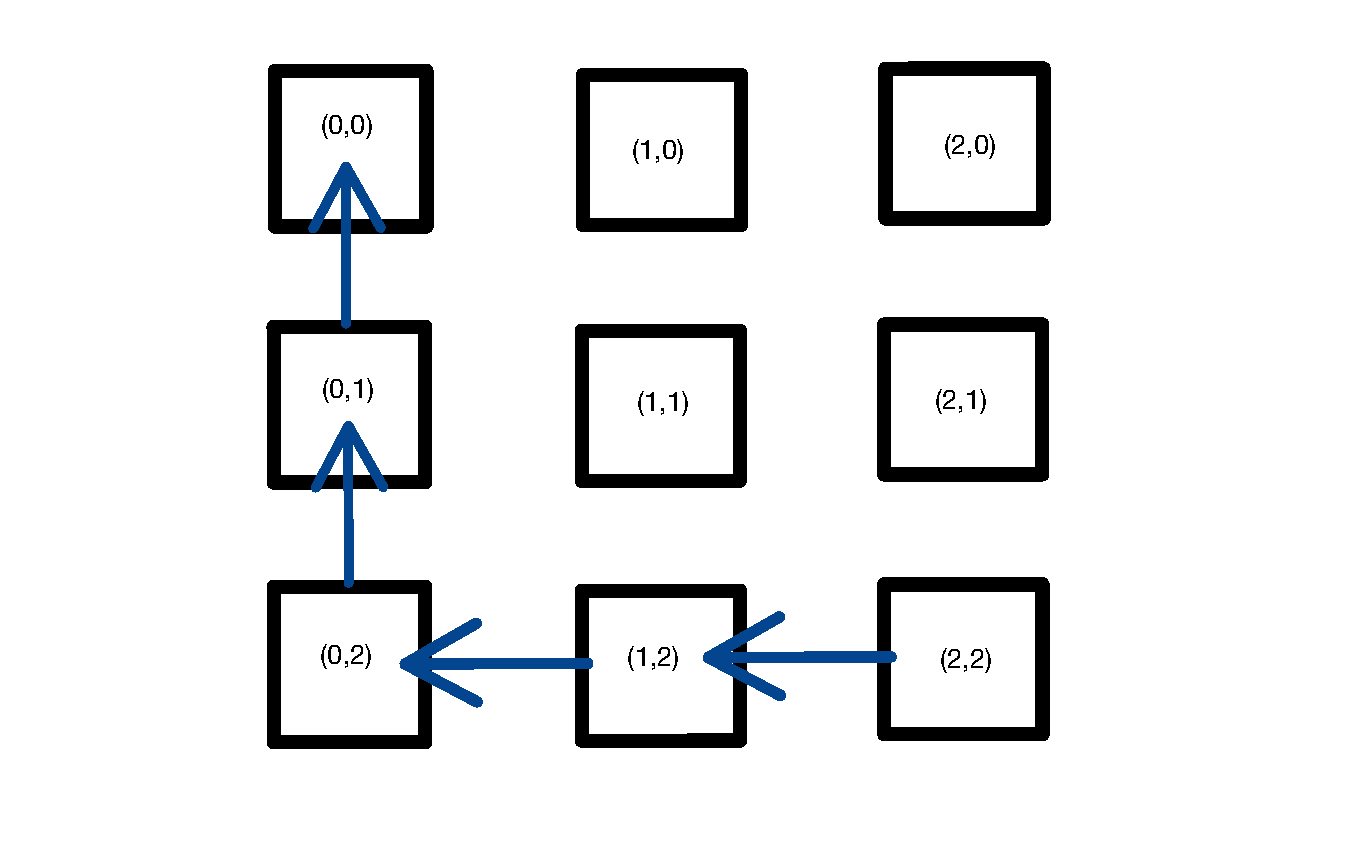
\includegraphics[width=\textwidth]{images/left_ex_read.pdf}
  \caption{Data Path in Left Readout}
\end{subfigure}
\caption{A left packet transaction example is shown. The packet transfers begin with the furthest node (2,2) receives a broadcast from the aggregator. 
The data are then sent to the "left" and then "up" towards the base node, and finally to the aggregator node.}
\label{fig:left_packet_drift}
\end{figure}


\subsubsection{Trunk Timing Example}

The final routing scheme we simulate we call the "trunk" routing.
We name this routing the "trunk" because all data are sent to a central column within the tile and then up towards the edge base node.
An example of a simple data transfer is shown in Figure~\ref{fig:trunk_packet_drift}.

For tiles of widths larger than three there are multiple choices for which column will be the trunk.
In for example, a 4$\times$4 tile can have either the second or third columns be the trunk.
In all even width cases we test, we choose the smaller row value for simplicity.
In the 4$\times$4 case we choose the second column and in the 8$\times$8 case, we choose the fourth (3,0) column instead of the fifth (4,0).

\begin{figure}
\centering
\begin{subfigure}{.5\textwidth}
  \centering
  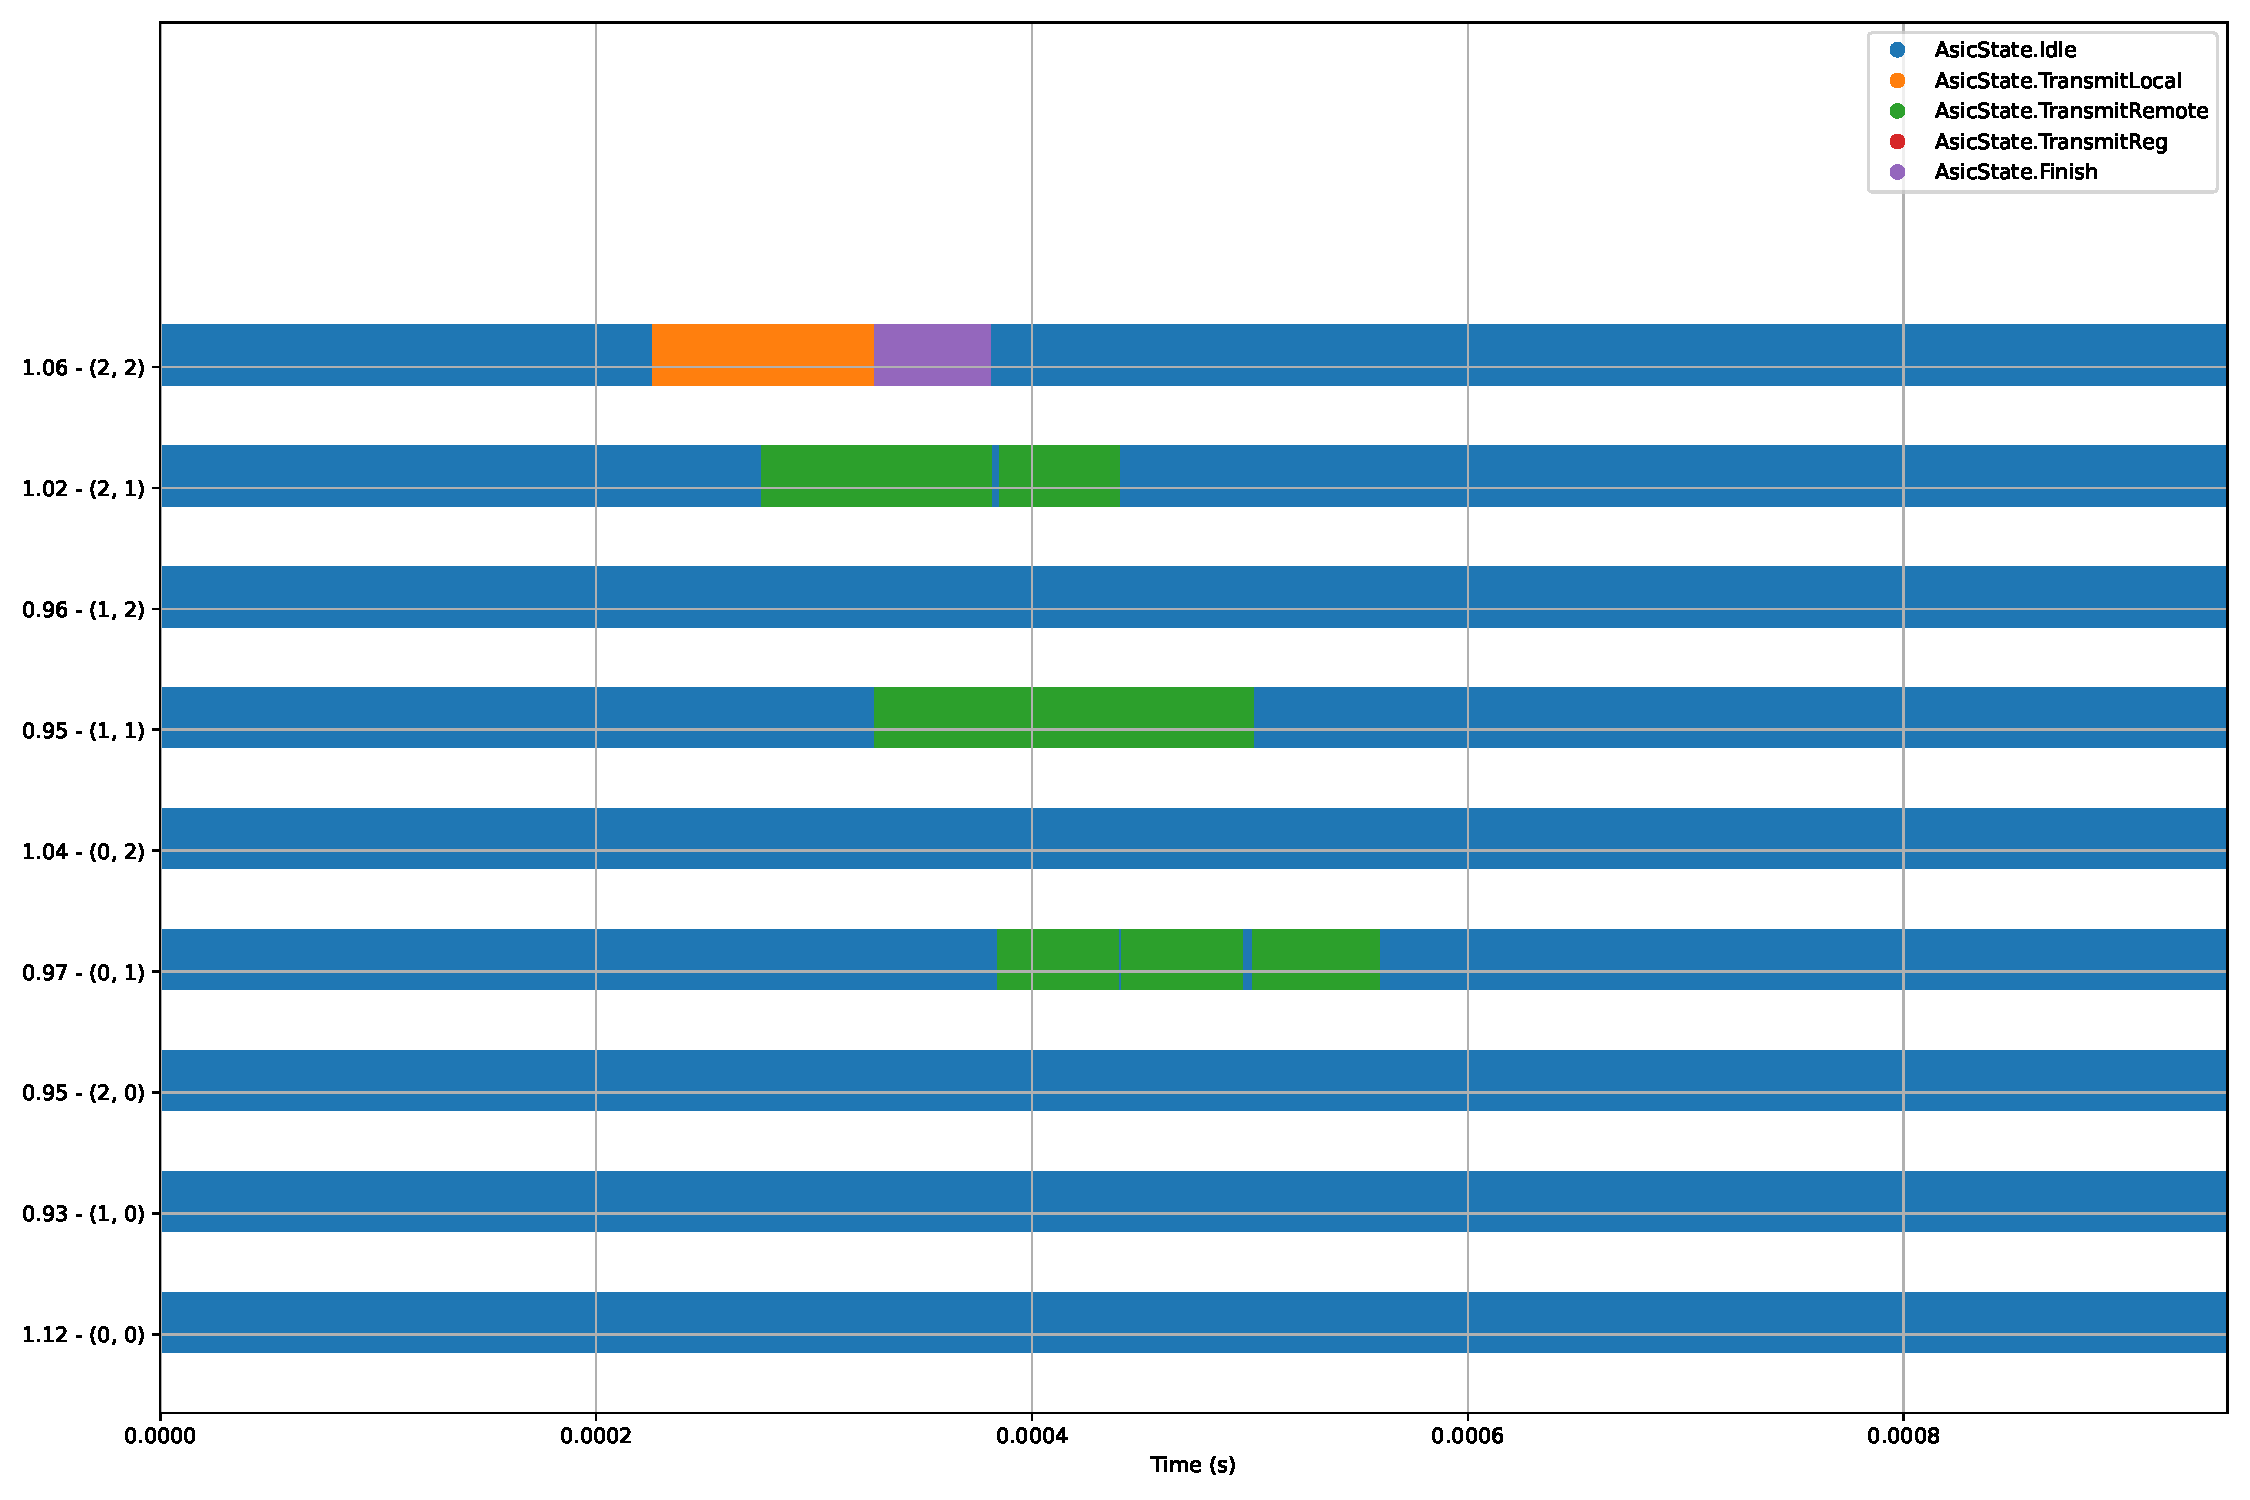
\includegraphics[width=\textwidth]{images/trunk_timer.pdf}
  \caption{Trunk Readout timing Diagram}
\end{subfigure}%
\begin{subfigure}{.5\textwidth}
  \centering
  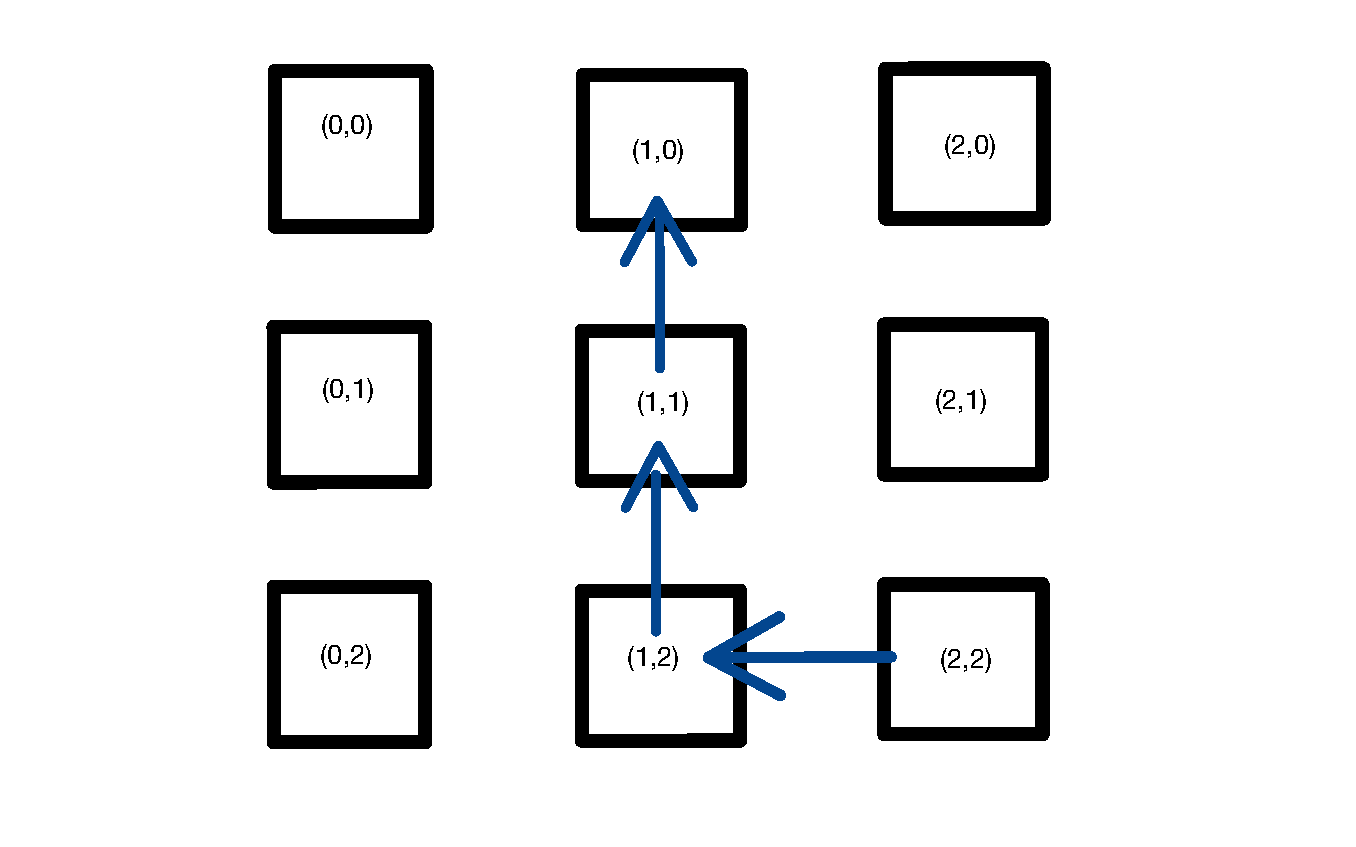
\includegraphics[width=\textwidth]{images/trunk_ex_read.pdf}
  \caption{Data Path in Trunk Readout}
\end{subfigure}
\caption{A trunk packet transaction example of two data words and a single event end word is shown. 
This routing method allows for the fastest possible transaction time since it minimizes the edge lengths between the base node and all other nodes within the tile.
In this 3$\times$3 example shown, the base node is at (1,0), or in the middle.}
\label{fig:trunk_packet_drift}
\end{figure}


\subsection{The Pull Architecture and FIFO Depths}

The "pull" architecture describes a tile configuration where data are only sent by ASICs within the tile when they receive a broadcast packet.
We describe an example simulation event in this section with the pull architecture and the three routing methods to demonstrate which variables are recorded.
The example presented in Figure~\ref{fig:local_buffer_hit_example} stores resets accumulated over ten seconds from both radiogenic backgrounds and a 3$\unit{GeV}~\nu_{e}$ event.
The data shown are the total local FIFO transactions (writes) that occurred in the ten second run.

The figures shown in~\cref{fig:snake_example_neutrino,fig:left_example_neutrino,fig:trunk_example_neutrino} demonstrate how the data are accumulated onto the remote FIFO depths for the snake, left, and trunk routings respectively.

%% example local hits
\begin{figure}[]
\centering
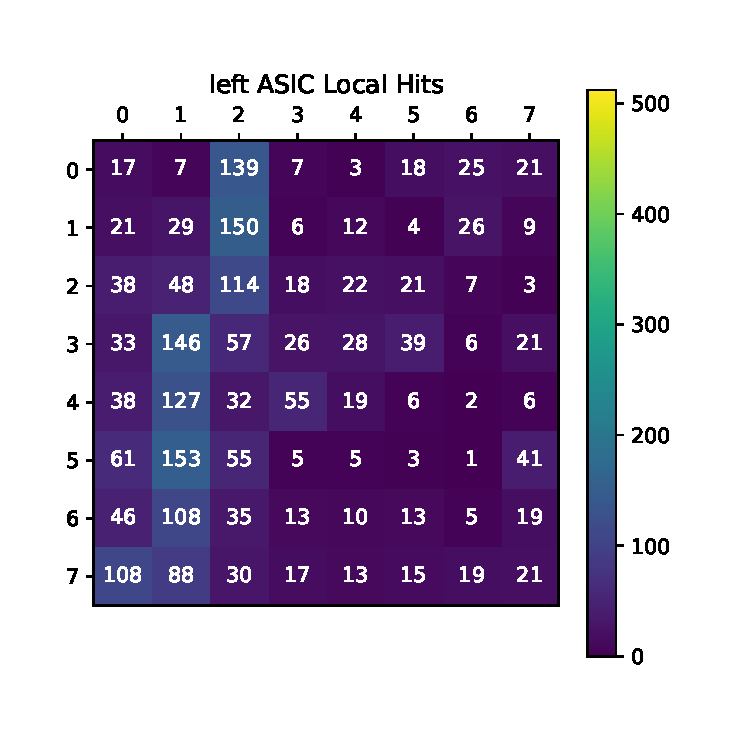
\includegraphics[width=0.75\textwidth]{images/left_asic_local.pdf}
\caption{Example local FIFO distribution of a $\approx 3\unit{GeV}~\nu_{e}$ event.
The numbers over each tile represent the total number of writes which occurred to each local FIFO in the array.
Even with the lowered resolution (each ASIC accounts for 16 pixels), different tracks are noticeable based on the FIFO depths.
The maximum scale for the heatmap is chosen to be 512 resets.
}
\end{figure}~\label{fig:local_buffer_hit_example}


%% example local vs remote of sneak
\begin{figure}
\centering
\begin{subfigure}{.5\textwidth}
  \centering
  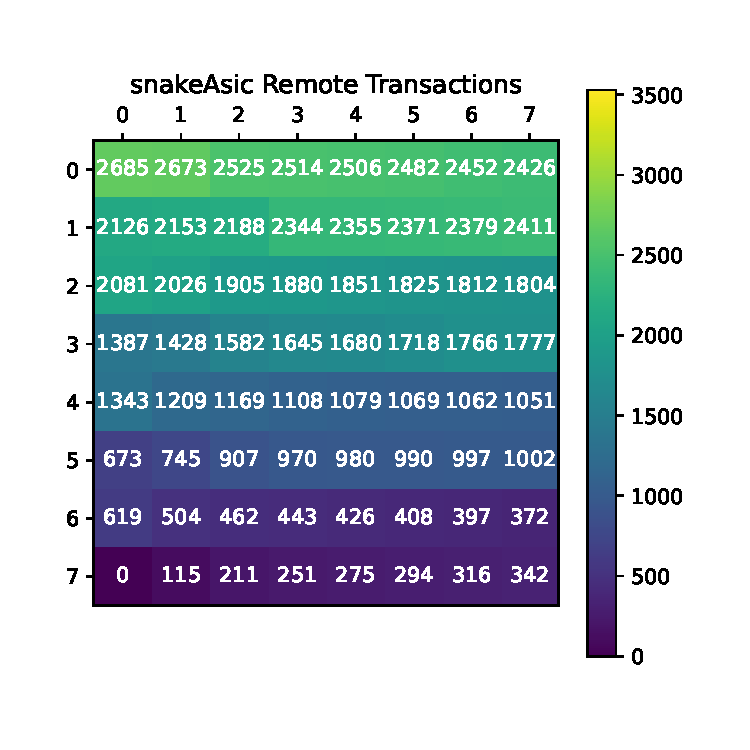
\includegraphics[width=\textwidth]{images/snake_asic_trans.pdf}
  \caption{Local FIFO Depths}
\end{subfigure}%
\begin{subfigure}{.5\textwidth}
  \centering
  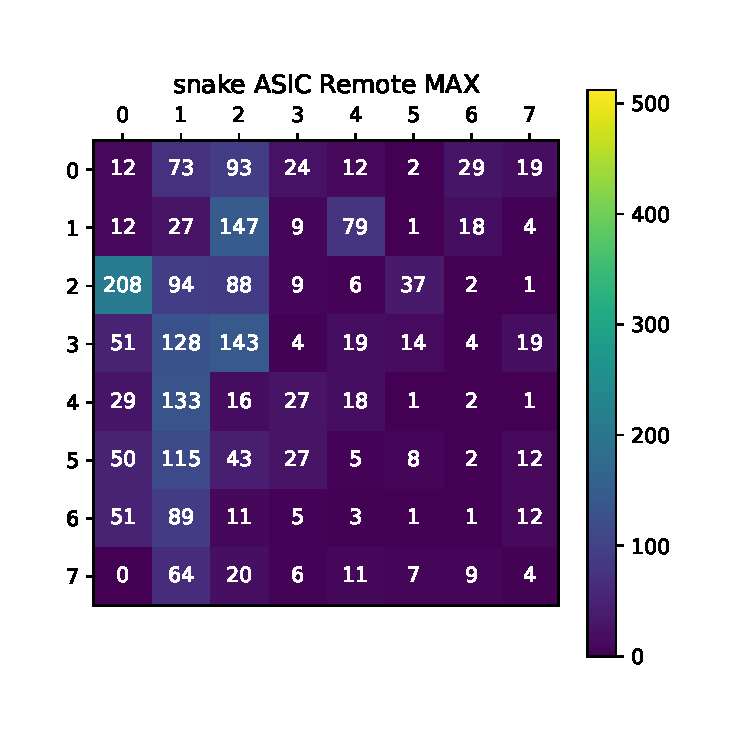
\includegraphics[width=\textwidth]{images/snake_asic_remote.pdf}
  \caption{Remote FIFO Depths}
\end{subfigure}
\caption{Example of local (a) and Remote (b) fifo depths of the example neutrino event from~\ref{fig:local_buffer_hit_example} after processing. 
The color bar to highlight the maximum number of transactions is used to indicate remote transactions which were happening for 2\% of the total readout time of 10 seconds.
The node which has the largest remote buffer depth corresponds to the ASIC with the slowest frequency as shown in Figure~\ref{fig:asic_frequency_example}.
The reason for this excess of buffer depth is due to packet buildup on the slow ASIC.
}
\label{fig:snake_example_neutrino}
\end{figure}


%% example local vs remote of left
\begin{figure}
\centering
\begin{subfigure}{.5\textwidth}
  \centering
  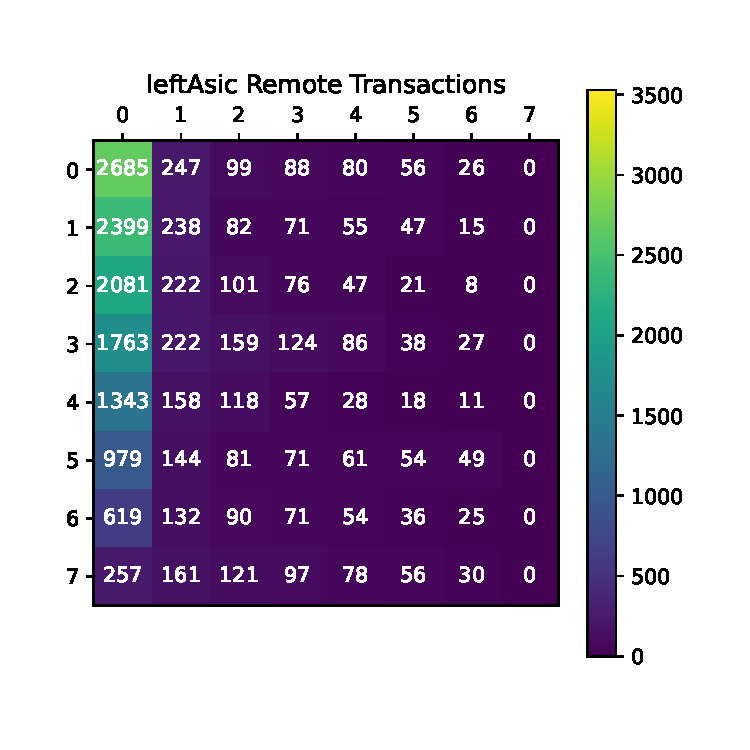
\includegraphics[width=\textwidth]{images/left_asic_trans.pdf}
  \caption{Local FIFO Depths}
\end{subfigure}%
\begin{subfigure}{.5\textwidth}
  \centering
  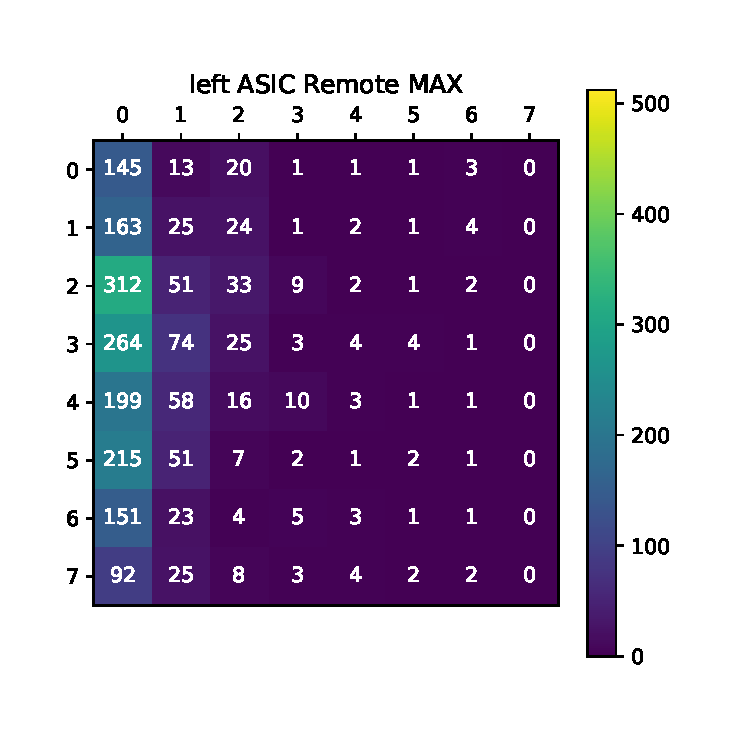
\includegraphics[width=\textwidth]{images/left_asic_remote.pdf}
  \caption{Remote FIFO Depths}
\end{subfigure}
\caption{Example of local (a) and Remote (b) fifo depths of the example neutrino event from~\ref{fig:local_buffer_hit_example} after processing.
 The ASIC which has the largest remote buffer depth also corresponds to the ASIC with the lowest frequency as shown in Figure~\ref{fig:asic_frequency_example}.}
\label{fig:left_example_neutrino}
\end{figure}

%% example local vs remote of trunk
\begin{figure}
\centering
\begin{subfigure}{.5\textwidth}
  \centering
  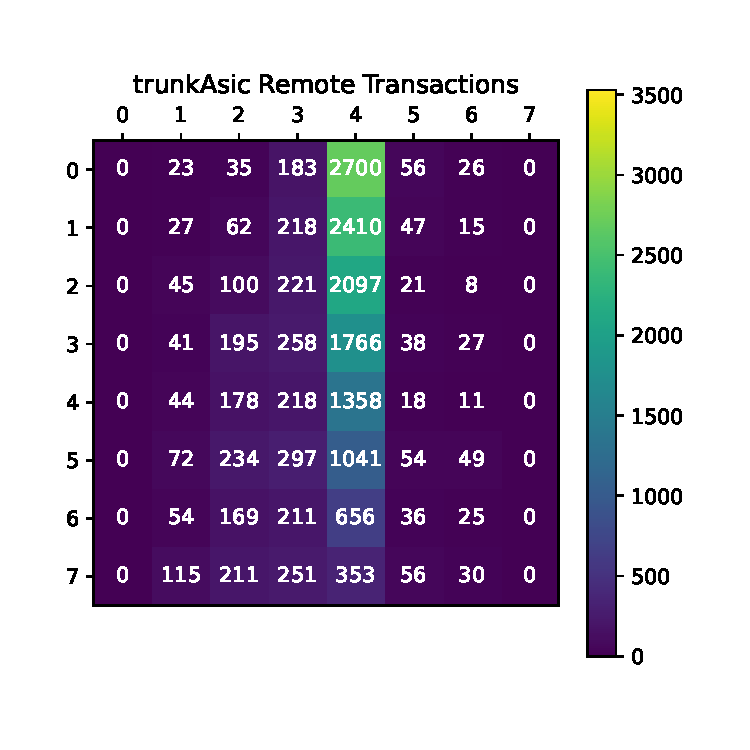
\includegraphics[width=\textwidth]{images/trunk_asic_trans.pdf}
  \caption{Local FIFO Depths}
\end{subfigure}%
\begin{subfigure}{.5\textwidth}
  \centering
  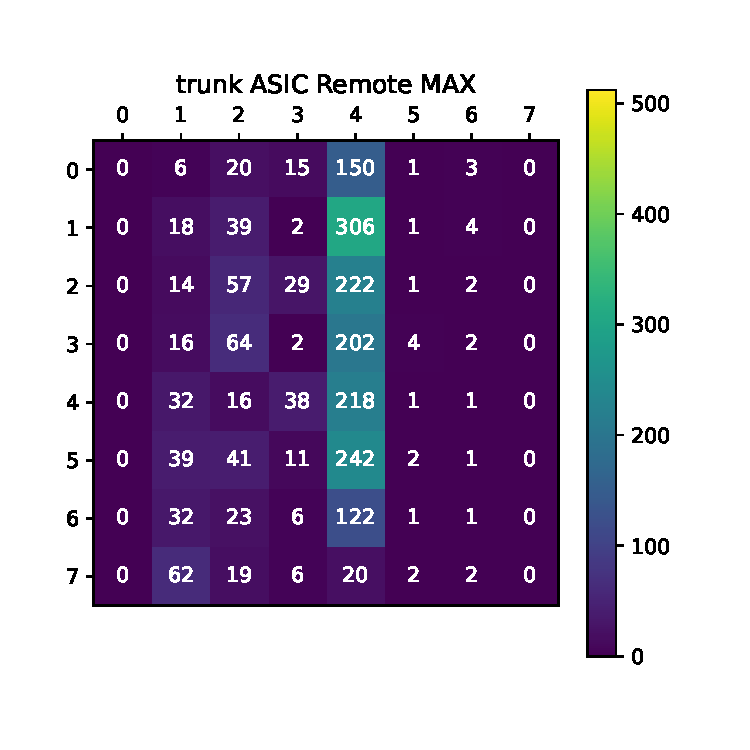
\includegraphics[width=\textwidth]{images/trunk_asic_remote.pdf}
  \caption{Remote FIFO Depths}
\end{subfigure}
\caption{Example of local (a) and Remote (b) fifo depths of the example neutrino event from~\ref{fig:local_buffer_hit_example} after processing.
The ASIC which has the largest packet buildup occurs at (4,1).
This ASIC also corresponds to the ASIC which has the lowest frequency along the trunk column as shown in Figure~\ref{fig:asic_frequency_example}.
}
\label{fig:trunk_example_neutrino}
\end{figure}


\begin{table}
\begin{center}
\begin{tabular}{|| p{20mm} | p{40mm} | p{40mm} | p{45mm} ||}
 \hline
 Routing & Local Max & Remote Maximum & Ratio of Remote:Local \\ [0.5ex]
 \hline\hline
  Snake & 153 & 208 & 1.36 \\
 \hline
  Left & 153 & 312 & 2.04 \\
 \hline
  Trunk & 153 & 306 & 2.00 \\
 \hline
 \hline
\end{tabular}
\caption{Example results obtained from the three simulation examples for the pull architectures shown in the previous figures.
The value of interest in determining the required remote FIFO depths for each ASIC is the maximum depth that occurred on any node.
A memory optimized routing configuration is one that would introduce the least strain on the remote buffer depths for a given local buffer depth input.
}
\label{table:example_analysis}
\end{center}
\end{table}

The following figures demonstrate why it is important to design all ASICs within a tile to meet the same specifications.
Future Q-Pix ASICs within a tile will be exposed to events at or above these energy scales, and there is no guarantee (until the ASIC is in hand) what the frequency of its oscillator will be, or its location within a tile. 
In all three routing examples shown it was not the base node which experienced the most strain on its buffer depth, but the ASIC along the route path which had the lowest frequency.


\subsection{The Push Architecture}

The final simulated parameter to describe is the push architecture.
Since the push architecture allows individual nodes to determine when packets can be sent all nodes must be inspected at each time step to check if a reset occurs before this new time window.
If a reset occurs at a time before the next simulation timestep, then the reset is removed from this node's hit list and is written to the node's local FIFO.
The node will then see at this simulation timestep that the local FIFO is not empty, and leave its idle state to send this packet.
An example of this process is shown in Figure~\ref{fig:push_arch_verification}.

Every simulated time step is shown and recorded along the x-axis.
The distance in time between simulation steps increases during packet transfers since the nodes state is fully determined during this time.
This simplification is performed to speed up simulation run time.

\begin{figure}[]
\centering
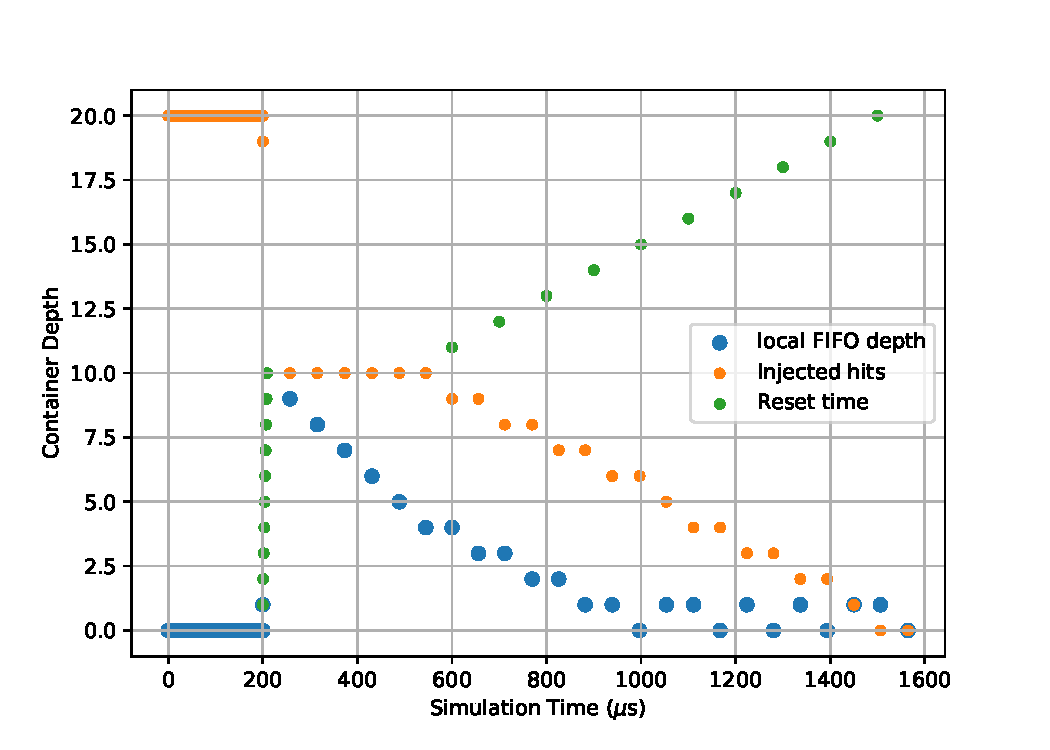
\includegraphics[width=\textwidth]{images/push_arch_buff.pdf}
\caption{A simulated push architecture with 20 injected hits at different times.
The time of the injected reset is indicated by the green points.
Before the simulation is run a node has its hits injected into a storage (orange) list.
Then, at each simulation time step ($\tau_{step}=1\unit{\mu s}$) the list is examined to see if a new hit will be written.
When a hit is found the relative time of the node can move forward in time to when this packet will be completed in time, while all other writes can occur to the local FIFO.
This is why the first local FIFO depth increases initially by one despite 10 nearly adjacent injected hits.
On the next time step, the depth then moves to nine; the simulation has sent the first of the 10 packets, and records nine.
This example correctly shows a maximum local FIFO depth of nine.
}
\end{figure}~\label{fig:push_arch_verification}

% describe the neutrino events here
\section{Physical Simulation Studies}
%% TODO - channel level heatmap for neutrino event

We now discuss the methodologies of the physical simulations used as input to the digital tile simulation described in the previous section.

\subsection{Radiogenic Backgrounds as a Calibration Source}

In this section we comment on the ability to, but do not perform, the auto-calibration of the reset loss per charge.
The full charge calibration procedure is beyond the scope of the work presented here, due to intracies that depend on the final implementation of the reset circuit as well as the replenishment circuit of the final Q-Pix ASIC.
Since this ASIC does not yet exist, the true verification of this methodology is not yet possible.
Nevertheless, we desribe the relevant portions to the problem here, since the charge calibration along with the frequnecy calibration and timestamp measurements determine Q-Pix's z-position reconstruction.

The main idea behind the auto-calibration of charge at the pixel level relies on using the known (and near constant) input current from the radiogenic backgrounds (mostly $^{39}$Ar) in the detetor. 
If a perfectly known and constant input current ($I_{o}$) source was input to a pixel it would produce a resets separated by a constant time ($\tau_{rtd}$).
It would be a straight foward matter to calculate the charge per reset: $Q_{o} = I_{o}*\tau_{rtd}$.

Then, to analyze the ability for an auto-calibration procedure for Q-Pix it is important to analyze and understand the long-running charge accumulation (resets) from backgrounds present in the LAr.
We use the following list of radiogenic sources of 10 distinct runs of 1000 seconds each.
Further details on radiogenic backgrounds in LAr can be found at~\citep{DUNE-FD_TDRv4:Abi_2020, ar39_backgrounds, phd_backgrounds}

\begin{table}
\begin{centering}
\begin{tabular}{|p{15mm} p{15mm} p{20mm} p{20mm} p{20mm} p{35mm} |}
 \hline
 Isotope & Rate [Bq/kg] & Region & Region Mass [kg] & Rate [Bq] & Number of Decays (per 10 s window) \\ [0.5ex]
 \hline\hline
  $^{210}$Po & 0.2 & PD [Bq/$m^2$] & 2.46856 & 0.493712 & 5 \\
  $^{60}$Co & 0.0455 & CPA & 90 & 4.095 & 41 \\
  $^{40}$K & 0.49 & APA & 258 & 1,264.2 & 12,642 \\
  $^{39}$Ar & 1.010 & bulk LAr & ~70,000 & 70,700 & 707,000 \\
  $^{42}$Ar & 0.000092 & bulk LAr & ~70,000 & 6.44 & 64 \\
  $^{42}$K  & 0.000092 & bulk LAr & ~70,000 & 6.44 & 64 \\
  $^{222}$Rn & 0.04 & bulk LAr & ~70,000 & 2800 & 28,000 \\
  $^{214}$Pb & 0.01 & bulk LAr & ~70,000 & 700 & 7,000 \\
  $^{214}$Bi & 0.01 & bulk LAr & ~70,000 & 700 & 7,000 \\
  $^{85}$Kr & 0.115 & bulk LAr & ~70,000 & 8050 & 80,500 \\
 \hline
\end{tabular}
\caption{The radiogenic background distribution is the same as that found in previous work~\citep{qpix:shion}.
For each 1000 ssecond analysis the pre-rounded values are scaled up by a factor of 100 to achieve the correct normalization of events for each isotope.
A key difference between the backgrounds is the origin or source of each background.
Of special note is $^{40}$K whose source location is the APA beams, and whose resets can be distinctly seen in Figure~\ref{fig:background_simulation} as the slightly more active (yellow) region of the APA.
Due to this source alone, it is likely that precise auto-calibration for charges will likely have to account for the pixel location within the APA.
}
\end{centering}
\end{table}
~\label{table:radiogenic_backgrounds}

The well-known C++ based Geant4~\citep{geant4:AGOSTINELLI2003250} simulation toolkit is used to simulate particle decay and ionizing particle interactions within the LAr volume.
We use the energy deposited along the track from each ionizing particle with the W-value for liquid argon (23.6 eV) to determine the number of electrons deposited in the LAr.
The resulting number of electrons are then unifromly deposited over the individual track.
Then we calculate the probability of recombination for each electron following the "modified box" model~\citep{2013JInst...8P8005A}.

The time and location of drift for each electron is calculated with an applied transverse and longitudinal diffusion with values taken from Table~\ref{tab:lar_prop}.
The simulations for all particle interactions are run individually with a uniform random sampling of the initial decay time interval within the 1000 second window.
All of the hits are then sorted by increasing time, so that the first hits read are the hits which occur the earliest.
Sorting the hits by time before accumulating charge ensures that the resets happen at the correct time.

This simulation procudes $\mathcal{O}(10^{11})$ hit interactions which produce $\mathcal{O}(10^{14})$ electrons, which in turn produces $\mathcal{O}(10^{9})$ resets.
To reduce the memory utilization of the simulation the electrons are accumulated on a hit-by-hit bases and are subdivided into a pre-determined 4$\times$4 cross-sectional area of the detector.
Each cross-sectional area defines a pixel.
The dimension of the LArTPC volume is 2.3~$\unit{m}$ $\times$ 6.0~$\unit{m}$ which divides into 575 pixels in the x-direction and 1500 pixels in the y-direction.
There are then a total of 862,500 pixels, which store location and reset information.

As an example, the total resets from 1000 seconds of the simulation are shown in Figure~\ref{fig:background_simulation}.
The most active pixel receives $\approx 220$ resets during this simulation time.
The bins for the histogram are at the pixel level, and represent the 4$\times$4$~\unit{mm^{2}}$ of each pixel.

\begin{figure}[]
\centering
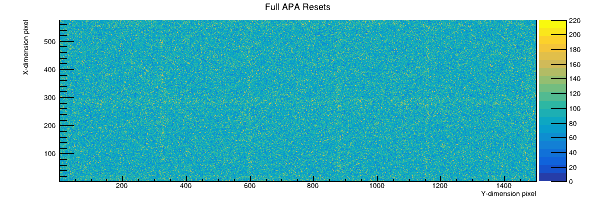
\includegraphics[width=\textwidth]{images/fullApaResets.png}
\caption{Full 1000 second of radiogenic background source simulation input into all pixels within the APA.
A close examination of the resets can reveal the additional resets from the backgrounds which are location dependent.
The majority of the uneven distribution of resets occur at the location of the APA bars due to the $^{40}$K isotope.
}
\end{figure}~\label{fig:background_simulation}

Additional information is tracked for each reset to identify the contribution of each radiogenic background for each reset.
A reset occurs when 6250 $e^{-}$ have accumulated on a pixel.
The time recorded for the reset is the same as the time the simulation calculates the last of the required 6250 electrons to arrive at the designated pixel region.
This optimization was added to the existing simulation framework to separate the unknown analog contribution to the timing uncertainty from the physical simulation.

In practice, the analog front-end reset circuit obviously takes time to respond to added charge and to issue a replenishment and reset commands.
There will always be some delay between the final electron's arrival, the time of the analog reset, the replenishment circuit, and the time recorded on the digital back-end.
However, for the purposes of this analysis, we assume that this reset and replenishment circuit activity can happen more quickly than the average local oscillator of the digital back-end. 
Therefore this analysis assumes the best timing measurement based on the digital back-end.
The time measurement is then limited only by the clock frequency of each local oscillator.
Finally, we comment that this optimization of the timing of the analog front-end affects only the time values, and by extension, the reconstruction of the particle tracks.
It does not affect the total amount of charge, and therefore the total number of resets recorded by each pixel.

Any combination of the backgrounds can contribute some or all of the electrons required to produce a reset.
The contribution of the total electrons for each of the radiogenic sources are shown in Figure~\ref{fig:compare_electron_contribution}.
We refer to the contribution of the number of the electrons to the reset as the "weight" of the reset.

\begin{figure}[]
\centering
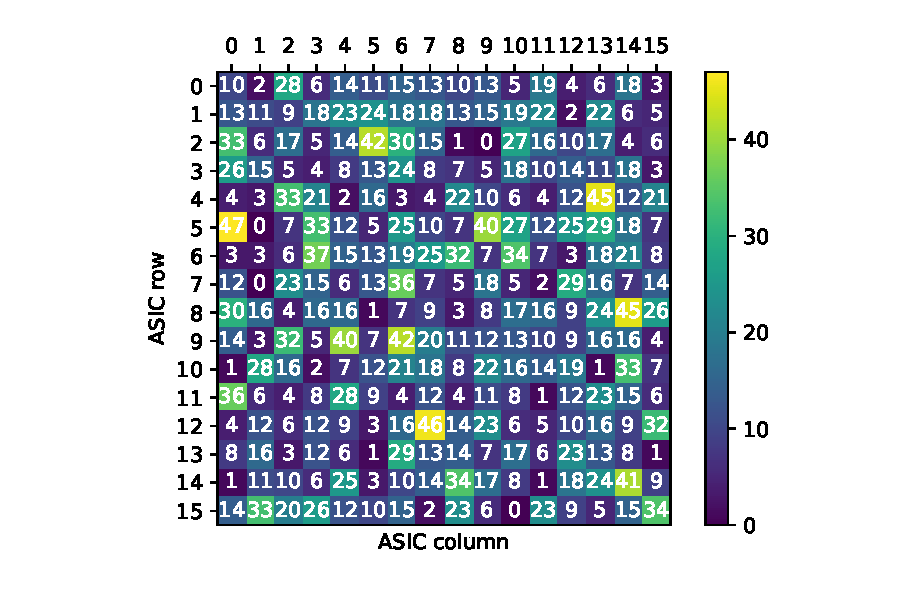
\includegraphics[width=\textwidth]{images/localHitsRadiogenic.pdf}
\caption{Baseline noise input for the digital simulation from all radiogenic sources and background leakage current. 
This figure shows the total resets in the 10 second window for the 16$\times$16 tile.
The other tile size configurations (4$\times$4, 8$\times$8, 10$\times$14) also use these reset data for background noise.
All tiles start with the top left node as their origin node.
}
\end{figure}~\label{fig:reference_input_noise}

%% example RTD for a 16x16 tile
\begin{figure}[]
\centering
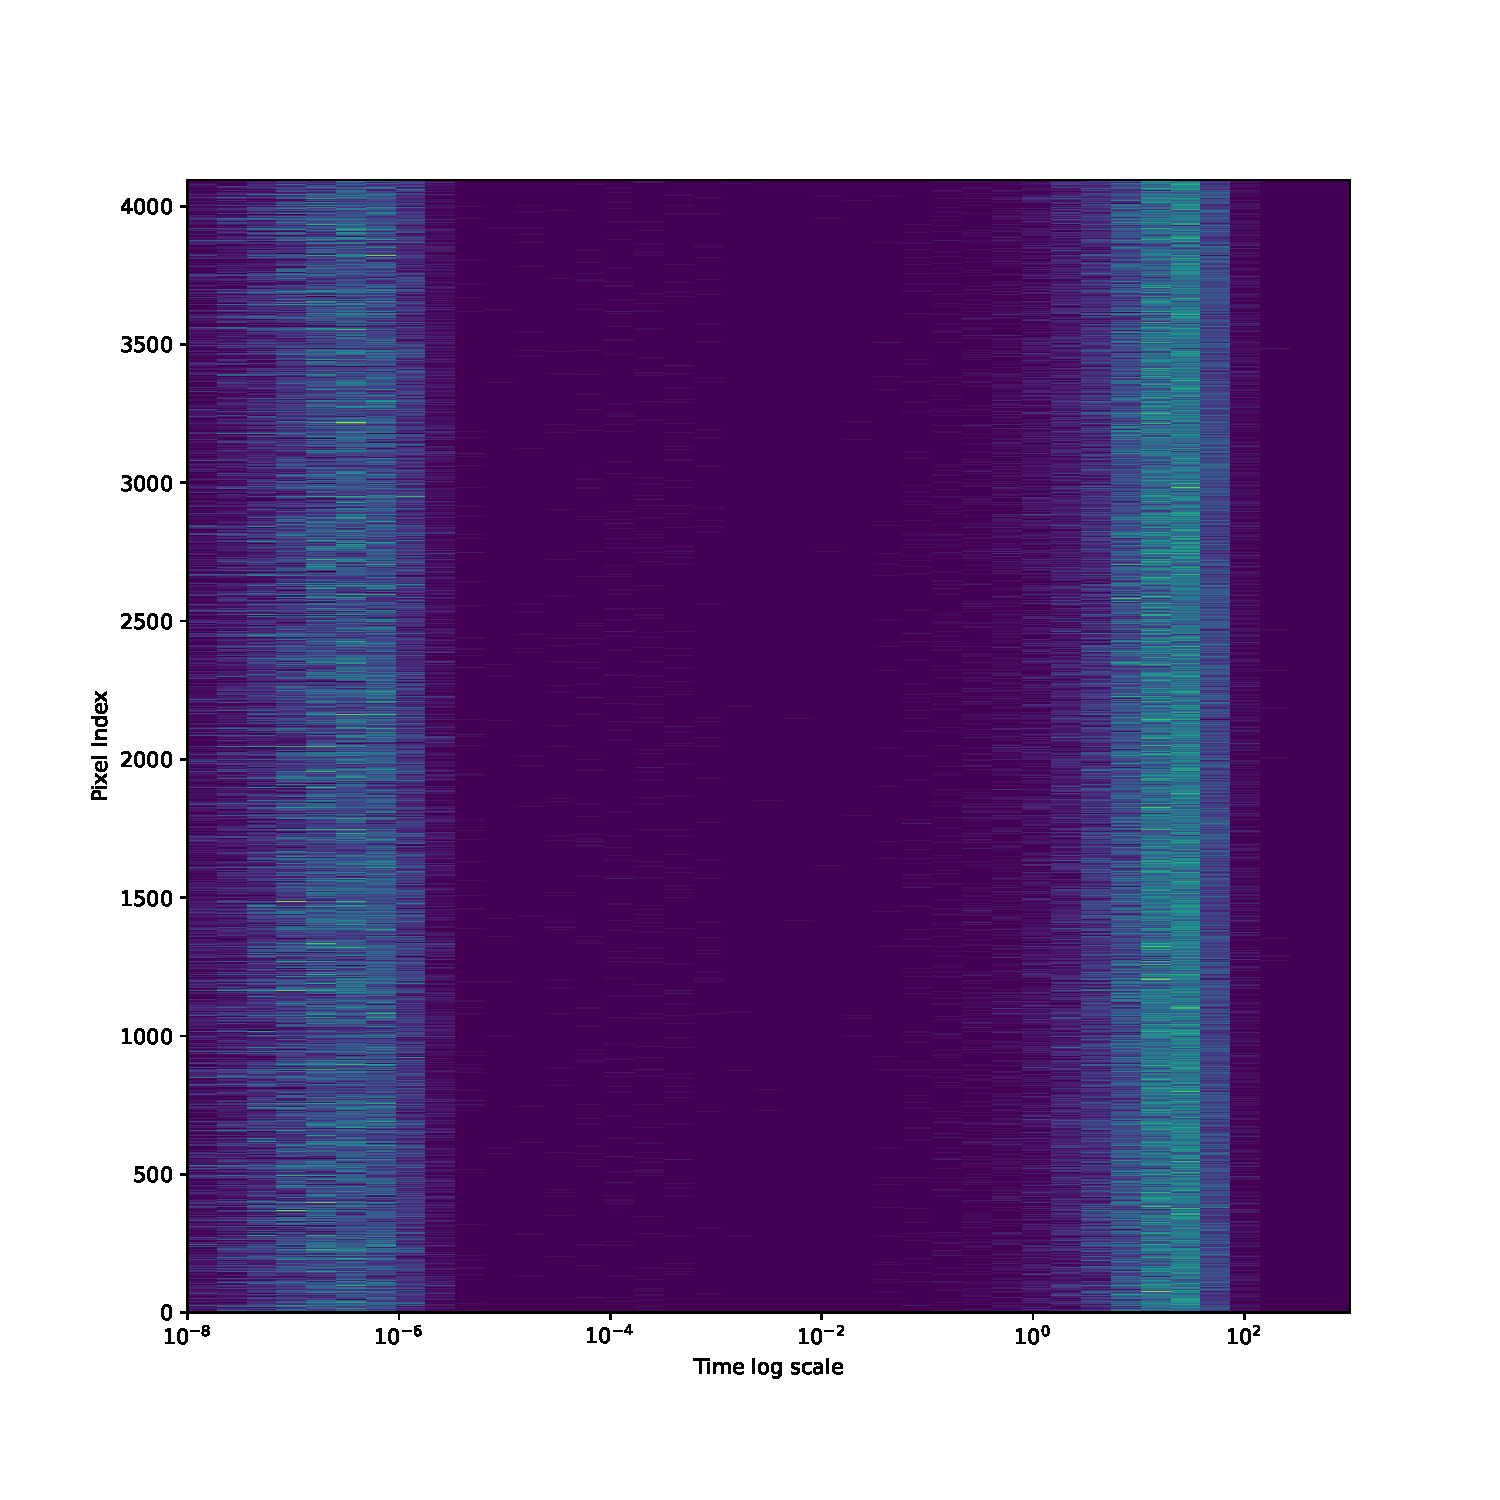
\includegraphics[width=\textwidth]{images/radiogenicRTDtimescale.pdf}
\caption{All 4096 pixels in the 16$\times$16 tile for 1000 seconds of radiogenic data. 
The y-axis represents a different pixel, and the x-axis is a log-scale time axis with even bin widths.
There are to clusters of resets for different time intervals.
The first large cluster of resets occurs at $\approx 10^{-7}$ seconds and is due to a single radiogenic decay event causing additional resets.
The second large cluster of resets occurs at $\approx$ 10 seconds.
This second cluster of resets is caused from the first reset of a new radiogenic decay event.
The ability to perform a charge calibration per pixel may depend on accurately resolving the mean for this "long period" RTD.
 }
\end{figure}~\label{fig:radiogenic_rtd_timescales}

%% time bin of 16x16 tile resets
\begin{figure}[]
\centering
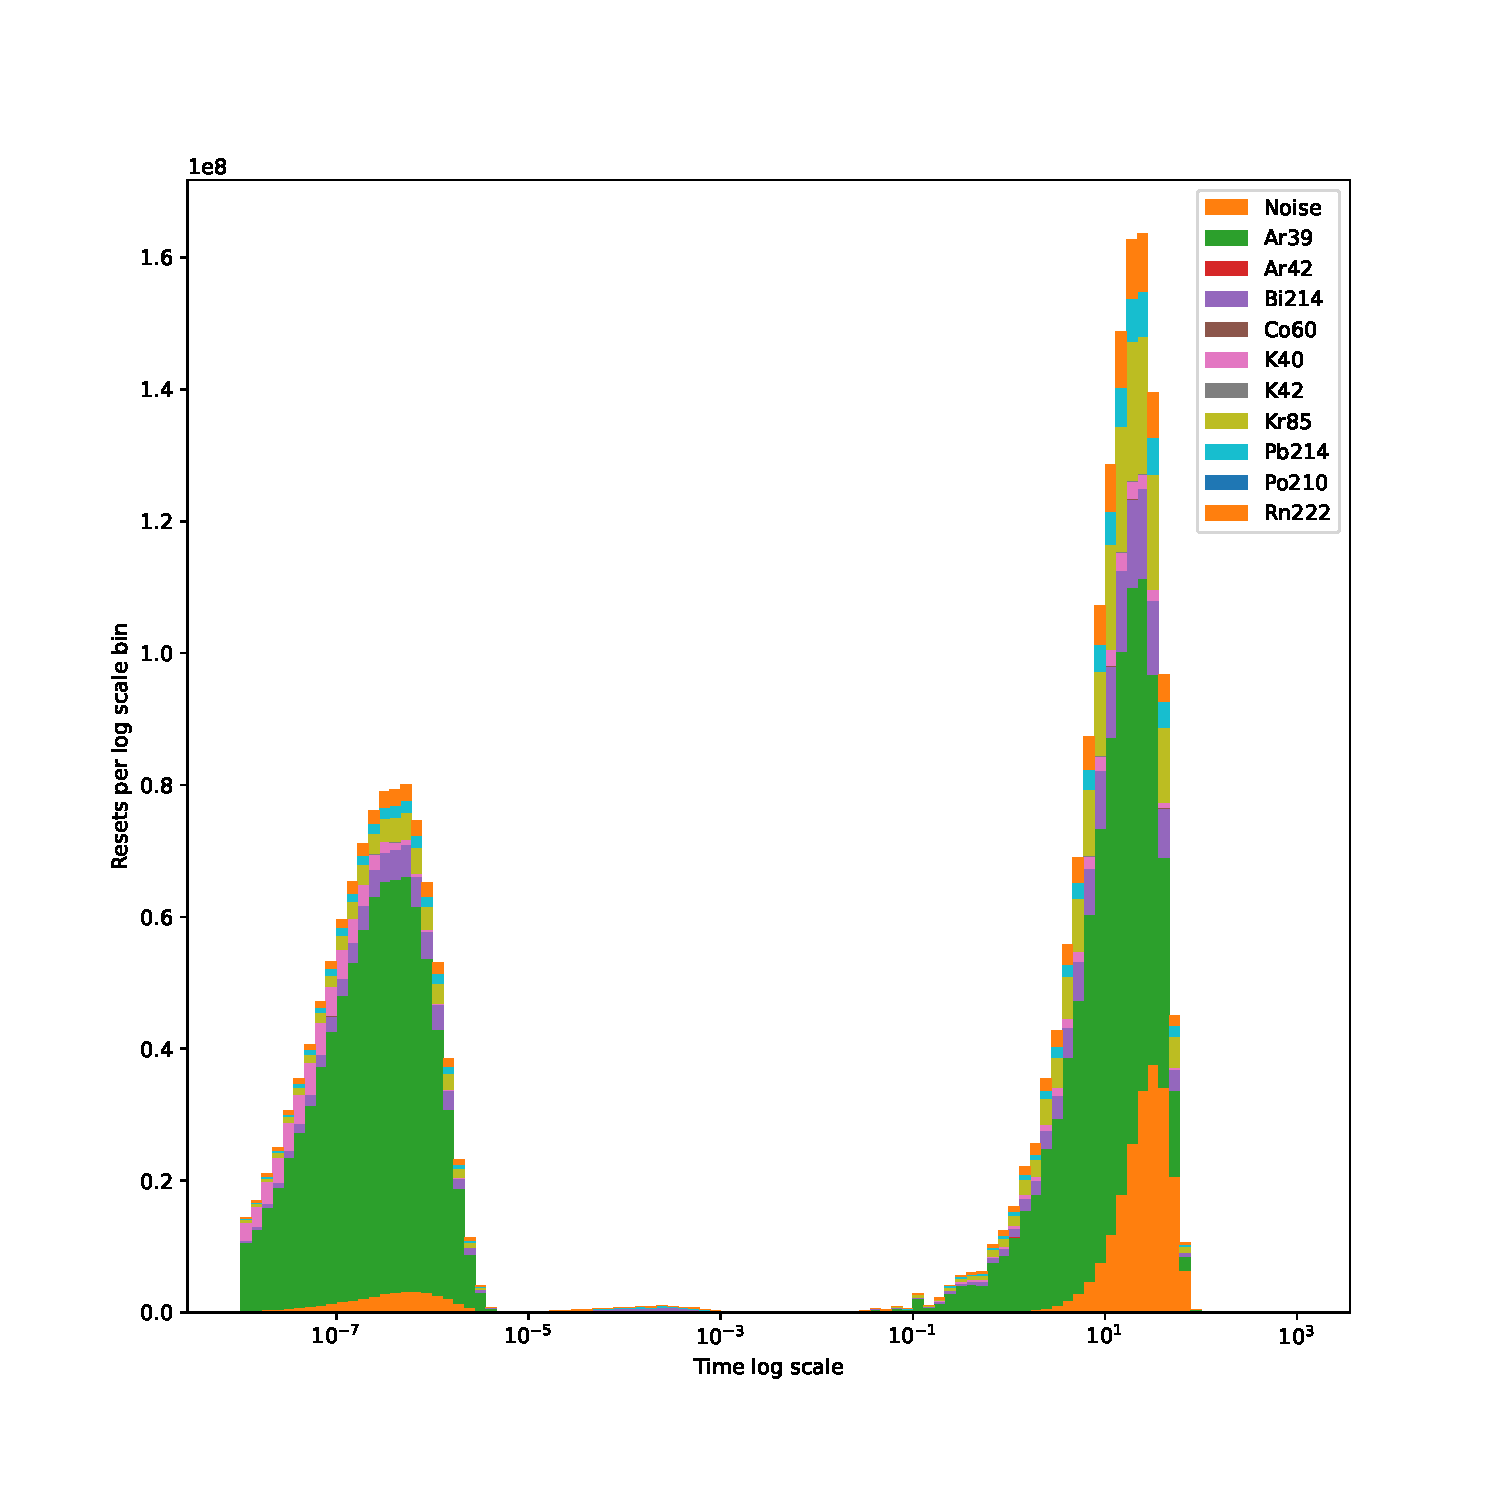
\includegraphics[width=\textwidth]{images/radiogenicRTDtimescale_stack_1d_noise.pdf}
\caption{All 4096 pixels in the 16$\times$16 array for 1000 seconds of radiogenic data. 
These data are the same as those shown in Figure~\ref{fig:radiogenic_rtd_timescales}, where all pixel RTDs are binned together.
There are two clusters of resets on two different time scales.
The first cluster of resets near at $\tau_{rtd} \simeq \mathcal{O}(10^{-7})$ is due to events which produce more than one reset.
The second cluster of resets near at $\tau_{rtd} \simeq \mathcal{O}(10^{1})$ are from a "waiting" period where there is no charge buildup from decays and only background noise.
The dominant source of electrons on each pixel is from the $^{39}$Ar, with a non-zero contribution from leakage.
The leakage current value used in this simulation is 10~\unit{aA}.
}
\end{figure}~\label{fig:radiogenic_rtd_timescales_comparing_no_noise}

The ability to perform a charge auto-calibration using radiogenic events depends on the background to provide a reliable average input current source.
We use only the data presented in Figure~\ref{fig:radiogenic_rtd_timescales} and calculate the mean time between resets for all pixels.
For this simple calculation, we simply take the total number of pixels (4096) and divide by the total number of recorded resets (411152) and obtain and average RTD of 9.96 seconds.

A very rough expectation of background current is $I_o \approx$ 100~\unit{aA}.
We can then use the following equation to calculate:
$$
I_{o} = \frac{Q_{o}}{\tau_{rtd}}
$$

solving for $Q_{o}$ with $\tau_{rtd} = 9.96$ and $I_{o} \approx 100$~\unit{aA}, we obtain:
$$
Q_{o} \approx 100*10^{-18} * 9.96 / 1.6*10^{-19} \approx 6225
$$

More sophisticated analysis will be needed for pixel level charge calibration.
The contrived derivation above assumes equal capacitance and charge replenishment on all pixels, which in practice is not necessarily true.
Furthermore, additional tests can likely be done for each pixel by comparing the peak of the distributions as shown in Figure~\ref{fig:radiogenic_rtd_timescales_comparing_no_noise}.
Such an analysis is not appropriate yet since it is not yet known what the leakage current will be in the Q-Pix ASIC.
As shown in both Figure~\ref{fig:radiogenic_rtd_timescales_comparing_no_noise} and Figure~\ref{fig:compare_electron_contribution}, the contribution from noise is not negligable.
Therefore, any true analysis of the charge auto-calibration ability of Q-Pix awaits studies of both the leakage current and replenishment circuits of the analog frontend.

\subsection{Reset Contribution of Radiogenic Sources and Leakage Current}

Figure~\ref{fig:compare_electron_contribution} compares the total (Plot-A) and percentage (Plot-B) electrons contributed from noise and radiogenic sources.
These results highlight the importance of understanding and mitigating any leakage current for every pixel.
A leakage current of 10~\unit{aA} contributes $\approx$ 10\% to the total background current.
What may prove difficult in the auto-calibration procedure of the Q-Pix readout is that while the contribution from radiogenic sources shown in Figure~\ref{fig:compare_electron_contribution} may be the same, the leakage contributions may not be.


%% graphic for energy deposited by source
\begin{figure}
\centering
\begin{subfigure}{.5\textwidth}
  \centering
  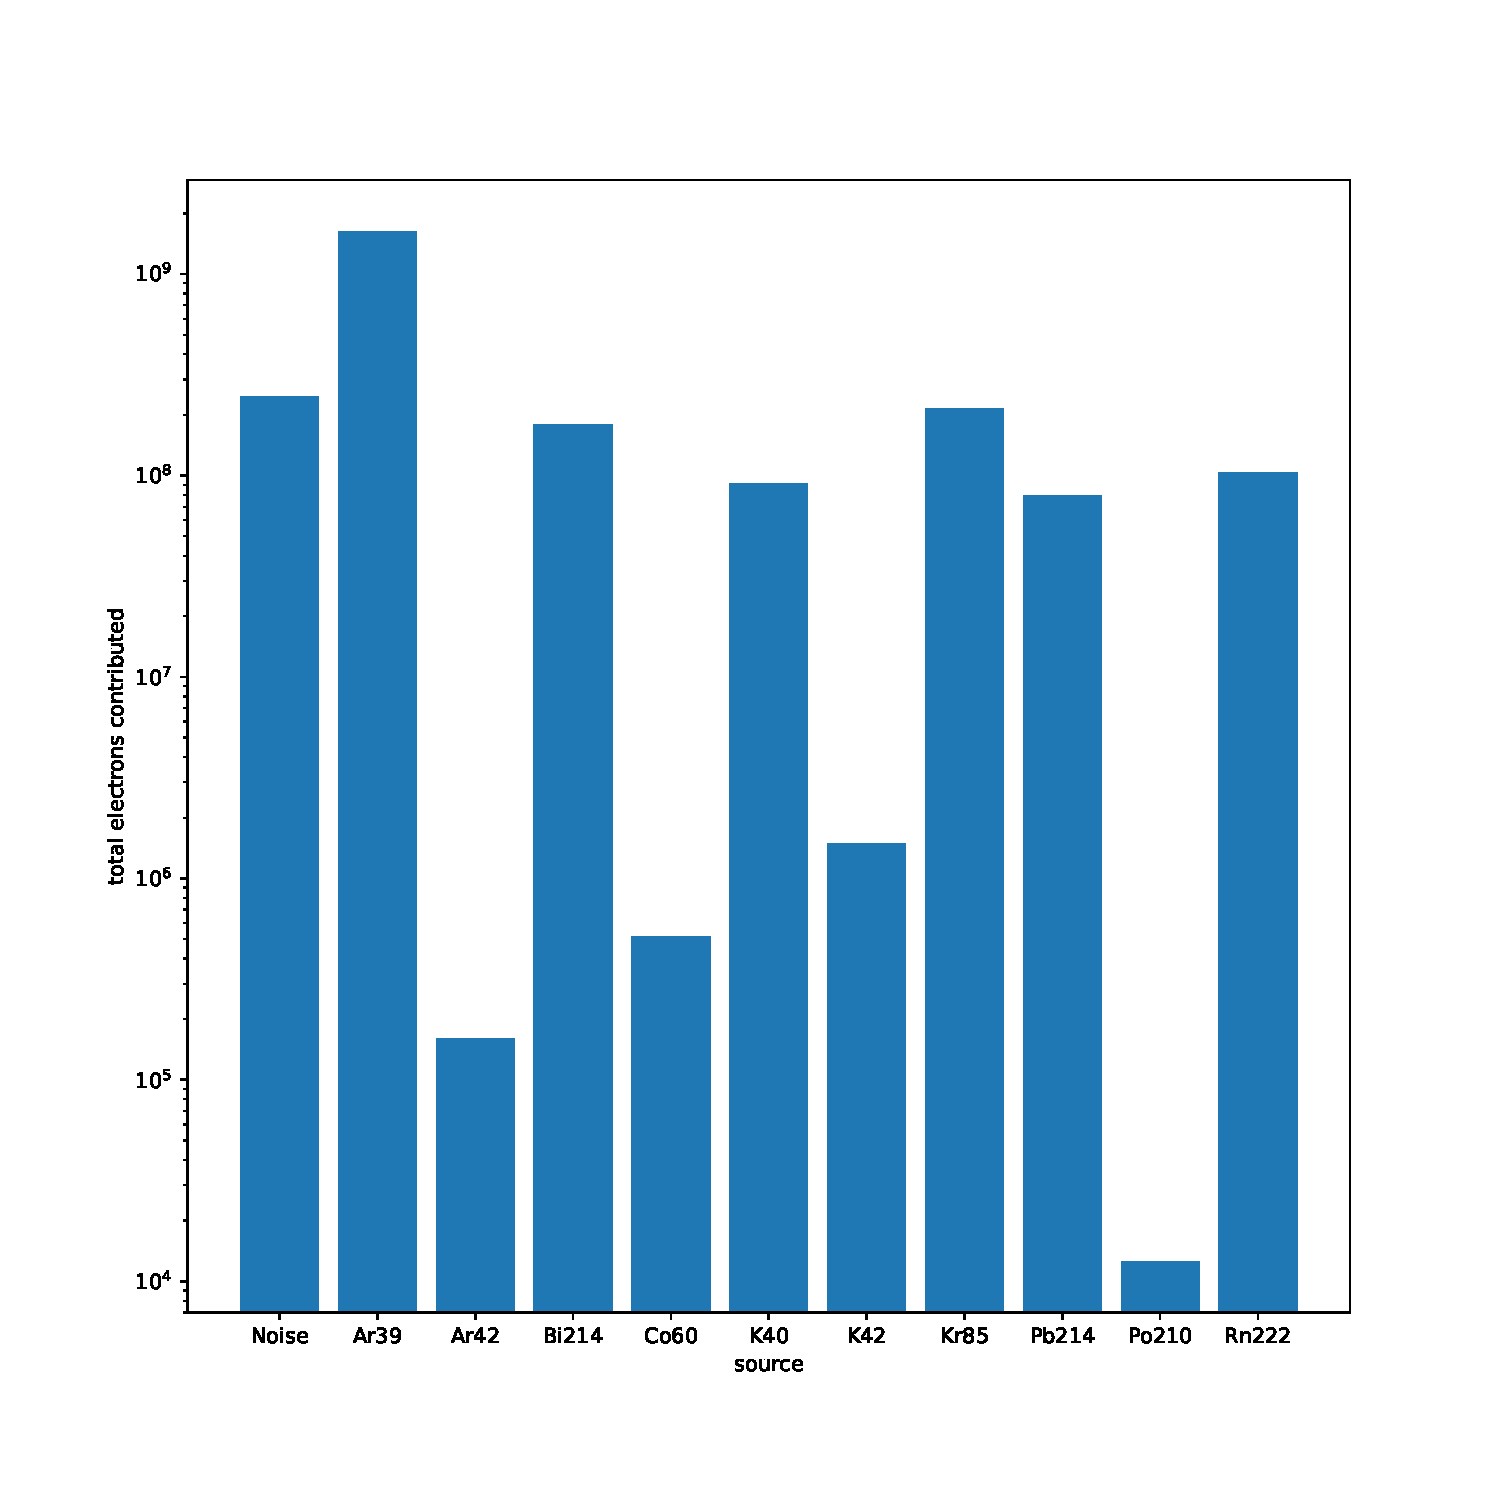
\includegraphics[width=\textwidth]{images/sim_electron_contribution_log.pdf}
  \caption{Contribution of total electrons.}
\end{subfigure}%
\begin{subfigure}{.5\textwidth}
  \centering
  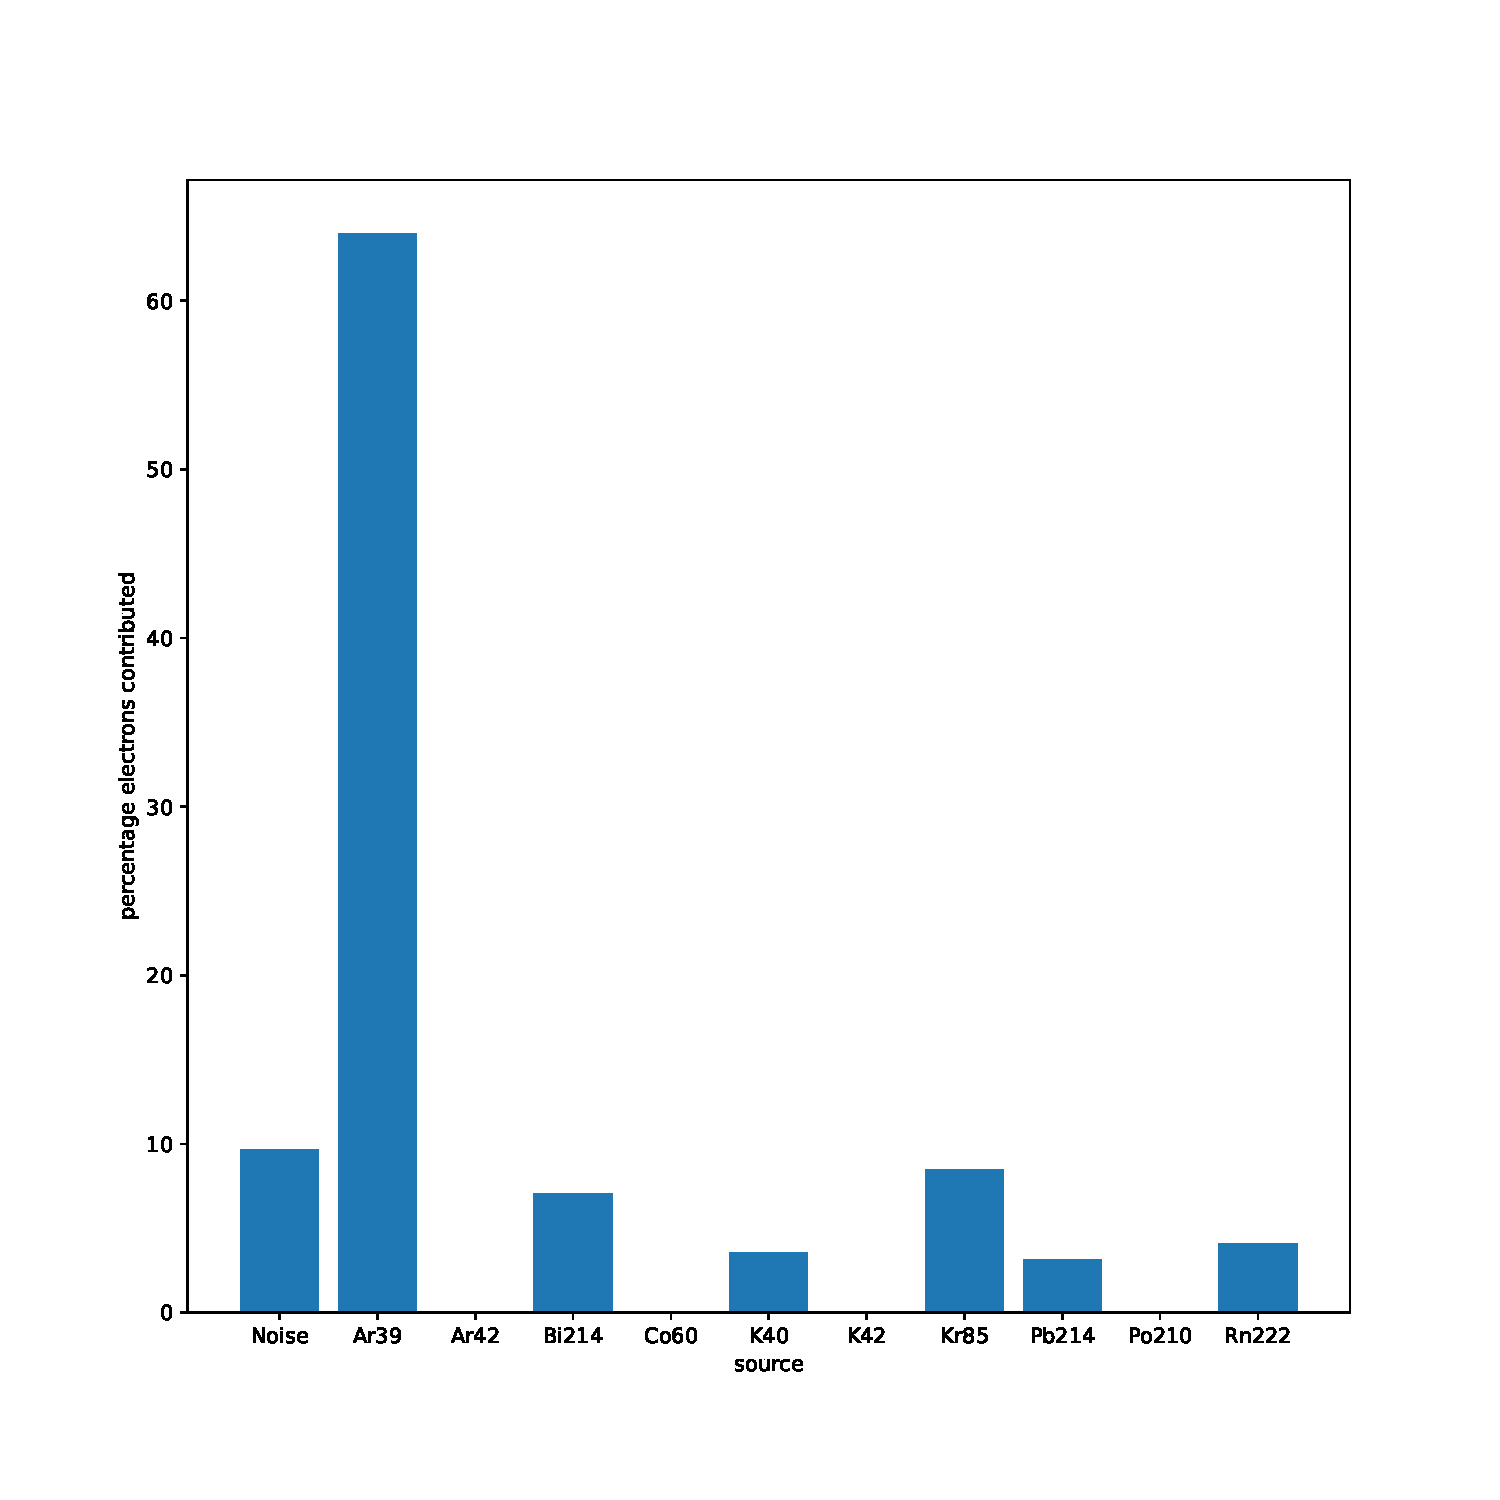
\includegraphics[width=\textwidth]{images/sim_electron_contribution_percent.pdf}
  \caption{Contribution of electrons by percentage.}
\end{subfigure}
\caption{Both figures indicate a comparison of the amount of electrons deposited on all pixels in the tile shown in Figure~\ref{fig:reference_input_noise}.
Plot (A) represents the total number of electrons on a log scale.
As expcted, $^{39}$Ar contributes the majority of background charge.
The leakage current used is 10~\unit{aA}, and represents about 10\% of the total contribution of electrons.
This implies that leakage currents from the front circuit which are $\approx 100$~\unit{aA} will contribute nearly as much electrons to the steady-state RTDs as the radiogenic backgrounds.
}
\label{fig:compare_electron_contribution}
\end{figure}

%%%%%%%%%%%%%%%%%%%%%%%%%%%%%%%%%%%%%%%%%%%%%%%%%%%%%%%%%%%%%%%%%%%%%%%%%%%%%%%%
%%%%%%%%%%%%%%%%%%%%%%%%%%%%%%%   Part 2   %%%%%%%%%%%%%%%%%%%%%%%%%%%%%%%%%%%%%
%%%%%%%%%%%%%%%%%%%%%%%%%%%%%%%%%%%%%%%%%%%%%%%%%%%%%%%%%%%%%%%%%%%%%%%%%%%%%%%%
\section{Neutrino Interaction Studies}~\label{sec:neutrino_studies}

Here we discuss the implementation of the digital framework within the high energy regime.
For this we use as an input neutrino events from the Long-Baseline Neutrino Facillity (LBNF)~\citep{dune_cdr_2016_arxiv} and take the unoscillated flux of neutrinos which were used in~\citep{dune_2021_near_detector_cdr}.
These neutrino flux are simulated using GENIE~\citep{Andreopoulos:2009rq}, v2.12.10.
The interaction distributions for both the forward and reverse horn current directions are shown in Figure~\ref{fig:neutrino_interaction_flux}.

We do not perform any calculation involving the oscillation on the input neutrino flux.
The reason for this is that the digital back-end should be able to fully record data from all possible $\nu_{l}$ events regardless of interaction type, not only the intended $\nu_{e}$ appearance spectra.
It is equally important for a future readout to be able to correctly tag noise ($\nu_{\mu}$, or $\nu_{e}$ from the beam, etc.).
For example, sensitivity to mass ordering and CP violation rely on the abiility to measure $\nu_{\mu}$ disappearance in addition to the $\nu_{e}$ appearance.

What will be shown in the upcomming sections is that capability of the digital back-end depends on the energy deposited in the volume of the LAr.
By the virtue that oscillations change only the flavor (not the energy) of the $\nu$, the constraints of the back-end do not depend on if more (or less) $\nu_{e}$ are measured compared to $\bar{\nu_{e}}$, provided the back-end is capable of fully measuring both events.
Furthermore, by using the unoscillated flux of the neutrinos at the near detector, the neutrinos will be of necessarily higher energy than the expected flux at the far detector.
The use of high energy helps in establishing what we will show as the upper-bound for the required local and remote FIFO depths for each ASIC.

\begin{figure}[]
\centering
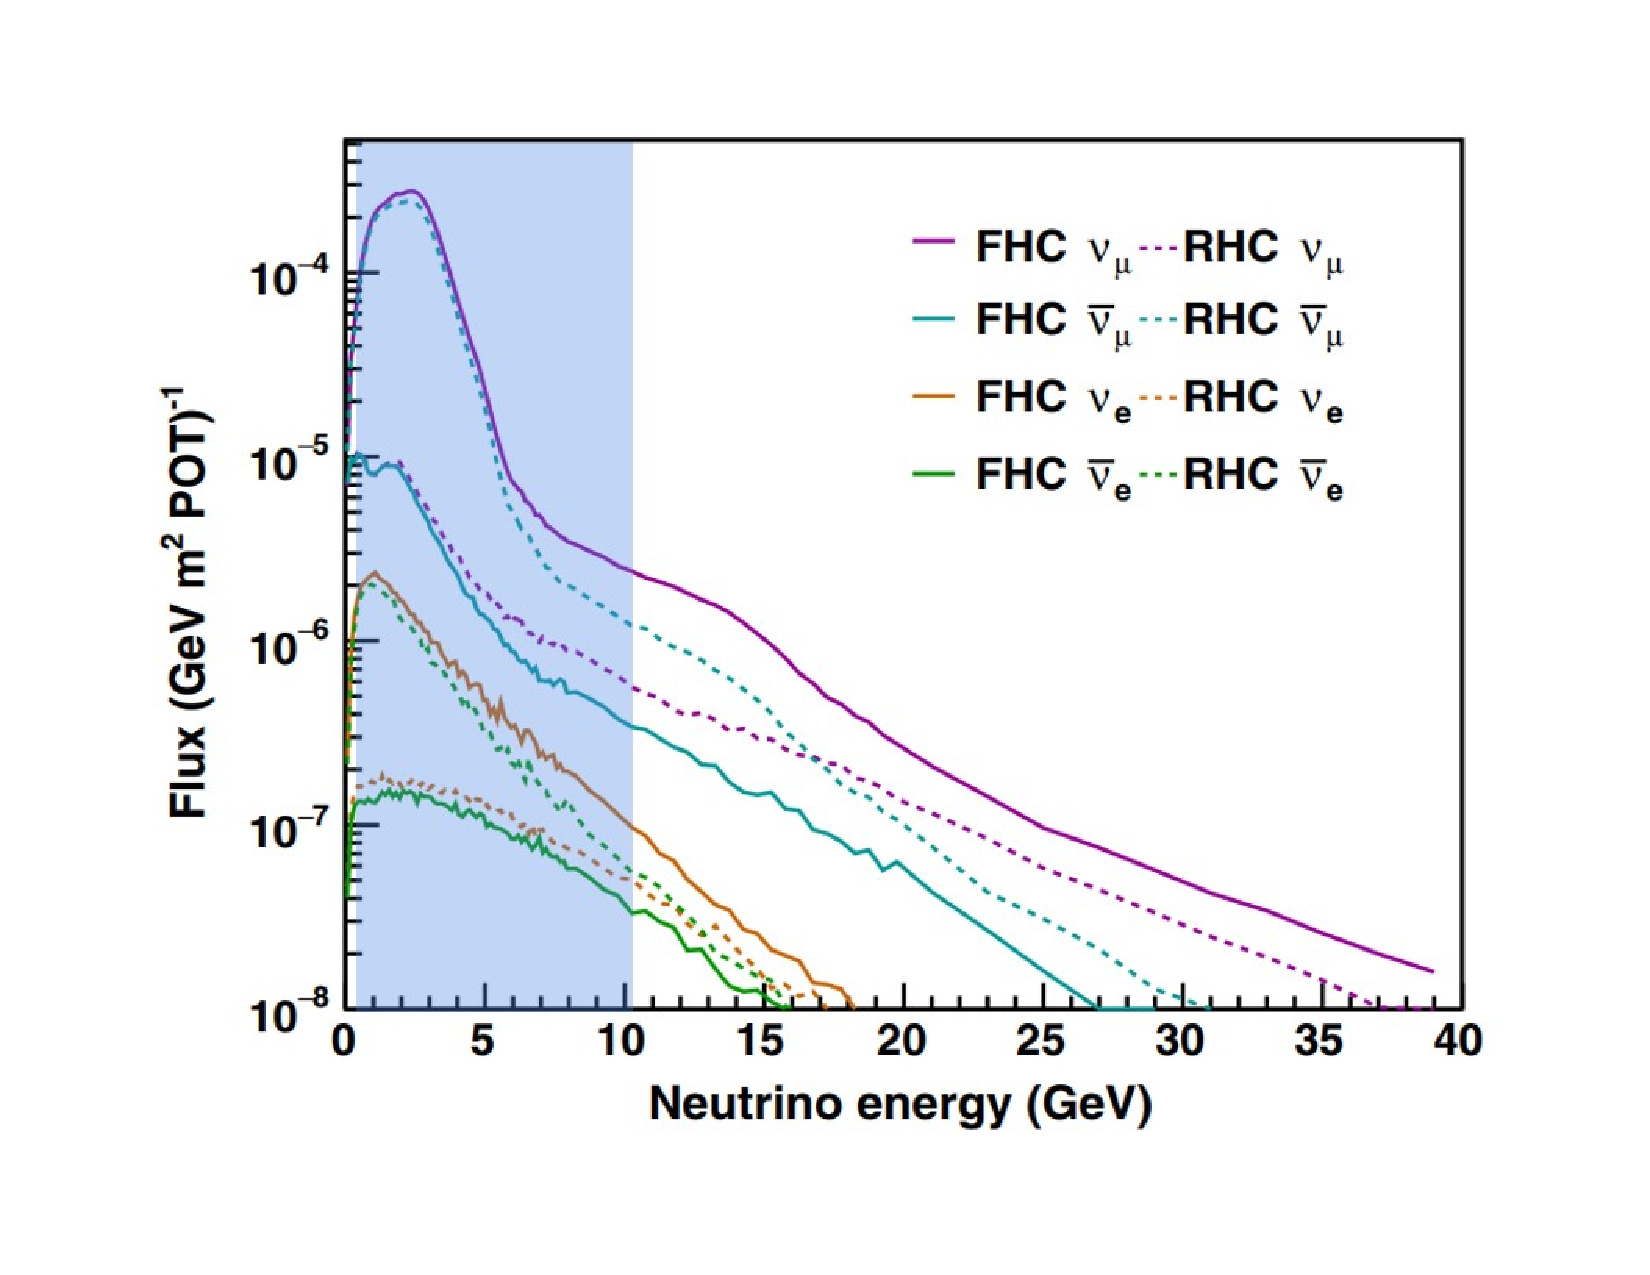
\includegraphics[width=\textwidth]{images/dune_flux_energy_range.pdf}
\caption{Flux spectrum of neutrinos from the neutrino beam used in this study. This figure is taken from~\cite{electron_flux_image_2020}. 
Highlighted in blue is the reconstructed energy range of neutrinos that are used to seed the interaction with the APA LAr's volume.}
\end{figure}~\label{fig:neutrino_flux}

\begin{figure}[]
\centering
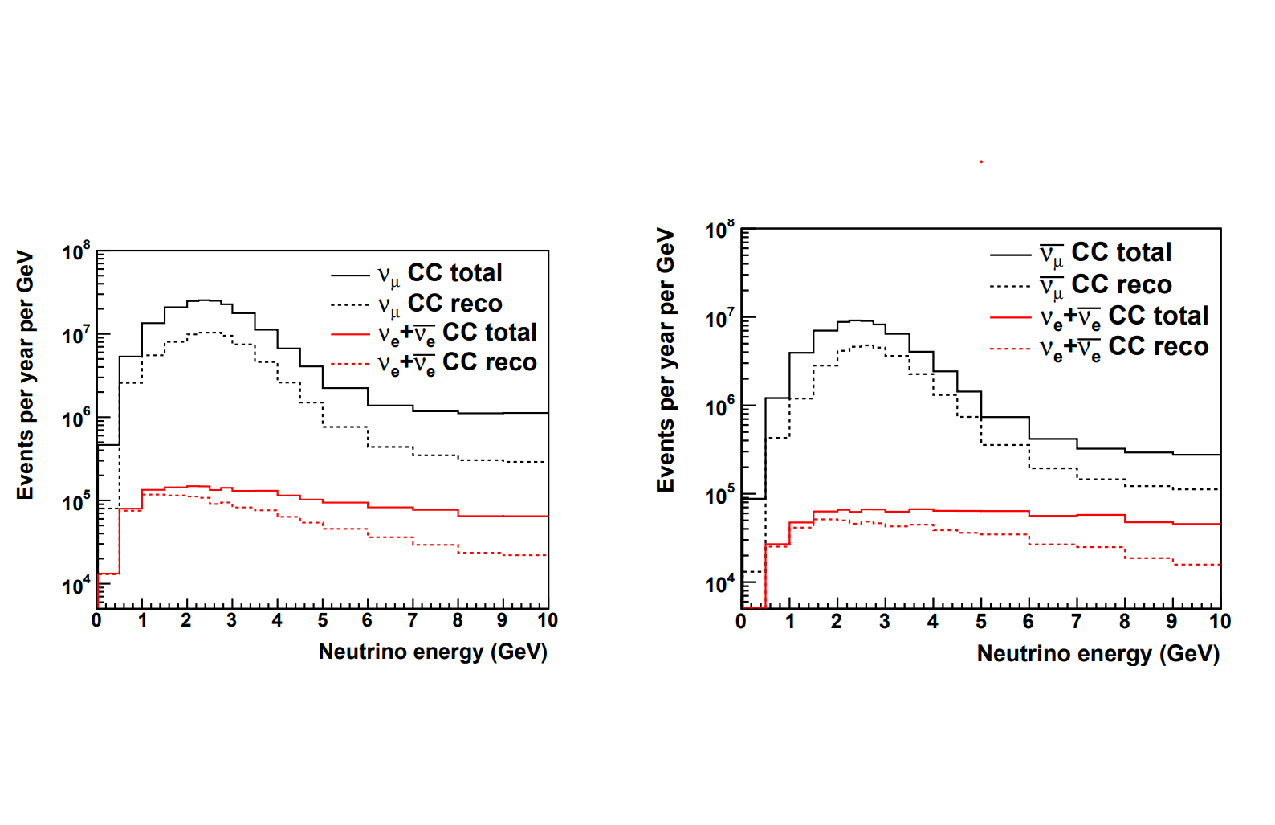
\includegraphics[width=\textwidth]{images/dune_cdr_2021_neutrino_flux.pdf}
\caption{Rate of CC neutrino interactions based on flavor as a functino of true neutrino energy.
Figure is taken directly from~\citep{dune_2021_near_detector_cdr}.
Right is shown the neutrino interaction distribution for the forward horn current.
The left image is for the reverse horn current.
Both images assume an average exposure rate of 1.2 MW from LBNF beam.}
\end{figure}~\label{fig:neutrino_interaction_flux}


\subsection{Neutrino Event Parameters}

Table~\ref{table:neutrino_params} describes the parameters of each input for the simulation.
The parameters used to vary the tiles for these neutrino input energies are shown on Table~\ref{table:tile_params}.

The Q-Pix readout presented here is designed for use in a LArTPC at the scale of DUNE-FD 10kT module~\ref{sec:dune}.
In order to test what kinds of requirements this readout will need we use high energy neutrino interactions as discussed in Section~\ref{sec:neutrino_studies}.
The different selection parameters for each event are neutrino flavor, neutrino energy, horn current direction, Z-position vertex position, and source neutrino momentum direction ($\theta_{z})$.
We define the beam direction (the direction parallel to the surface of the APA) as $\theta_{z} = 0$.
The X and Y positions are held constant for all interactions, at X = 120~\unit{cm} and Y = 3200~\unit{cm}.
The coordinate system we use, as well as a slice of the APA within a module are shown in Figure~\ref{}.

The LBNF beam is not the only source of high energy particles DUNE will detect.
Other high energy ($\simeq 10$~\unit{GeV}) interactions may come from other sources.
These other high energy events (such as nucleon decay, cosmic neutrinos) may also deposit energy on~\unit{GeV} scales per interaction.
These sources may interact with their net momentum vector pointing in any direction.
For this reason we also test $\nu_{e}$ and $\nu_{\mu}$ interactions at $\theta_{z} \pm$ 90~\unit{\degree}; this direction causes the secondary ionizing particles to carry momentum along the direction parallel to the pixel's surface normal.
These two momentum directions, though unphysical for beam interactions, still present possible interactions types within the scope of DUNE's propossed physics program~\citep{DUNE_TDRv3_Abi_2020}.

\begin{table}
\begin{center}
\begin{tabular}{|| p{30mm} | p{30mm} | p{90mm} ||}
 \hline
 Name & Values & Relation \\ [0.5ex]
 \hline\hline
  $\nu_{l}$ & $\nu_{e}$, $\bar{\nu_{e}}$, $\nu_{\mu}$, $\bar{\nu_{\mu}}$ & Oscillation measurements require sensitivity to measurements for both $\nu_{e}$ appearance, and $\nu_{\mu}$ disappearance.\\
 \hline
  $\nu_{l}$ Energy & 0.25~\unit{GeV} to 10~\unit{GeV}, in steps of 0.25~\unit{GeV} & neutrino energy determines output secondary energy, which causes more resents and directly affects buffer depths. \\
 \hline
  Horn Current & Forward and Reverse & Beam horn current direction affects neutrino flux, as shown in Figure~\ref{fig:neutrino_flux}. Additionally, mass heirarchy measurements (according to the MSW effect~\citep{Smirnov2004TheME}) require difference in measurements of appearance probability for $\nu_{e}$ and $\bar{\nu_{e}}$. \\
 \hline
  Z-position & 10~\unit{cm}, 80~\unit{cm}, 180~\unit{cm}, 280~\unit{cm}, 350~\unit{cm}  & Interaction z-position above the anode plane. Interactions which happen further from the collection plane have more time to diffuse or recombine. \\
 \hline
  $\theta_{z} $ & 0\unit{\degree}, $\pm$2\unit{\degree}, $\pm$90\unit{\degree} & Different momentum angles are different Z-positions, in general, direct ionized particle tracks within the active volume. \\
 \hline
\end{tabular}
\caption{The different neutrino simulation parameters which are passed into Geant4 based simulation.
  The original interaction products are generated using GENIE~\citep{Andreopoulos:2009rq} v2.12.10.
  The output products of the neutrino interaction produced from GENIE are then configured using the different parameters described above.
  We select $\nu_{l}$ events for different energies in bin-widths of 250 MeV; We follow the same bin width as is done in~\citep{DUNE_FD_TDRv2_2020} for their neutrino oscillation analysis.
  A selection of 100 events for each $\nu_{l}$ is taken within each energy bin, for a total of 3900 $\nu_{l}$ events for each horn current direction, z-position, and $\theta_{z}$ selection.
  Since there are two current directions, four $\nu_{l}$, five z-positions, and five $\theta_{z}$ positions, a total of 780,000 neutrino events are simulated.
}
\end{center}
\end{table}
~\label{table:neutrino_params}

%% fig example neutrino event
% image example of a full event with rotations
\begin{figure}
\centering
\begin{subfigure}{.5\textwidth}
  \centering
  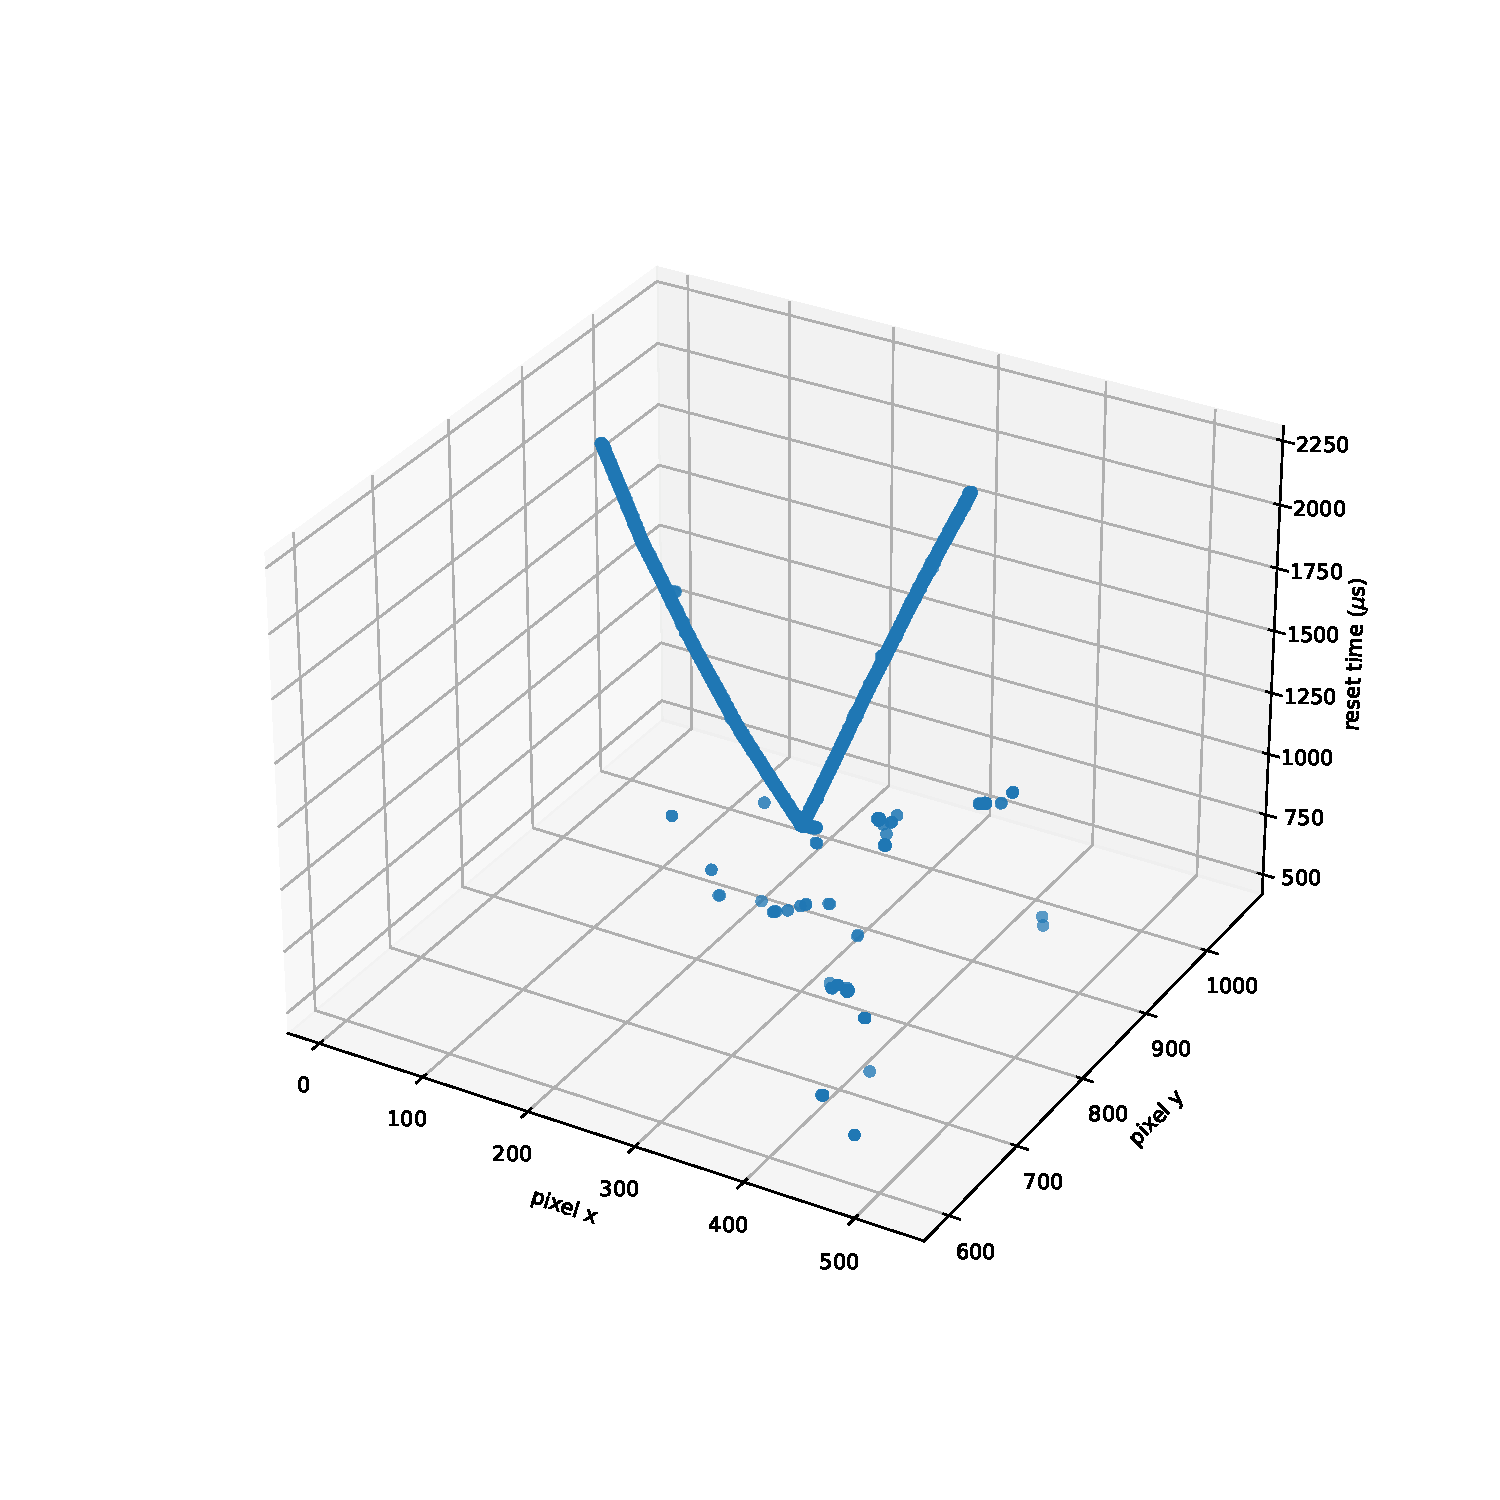
\includegraphics[width=\textwidth]{images/example_zdir_scatter.pdf}
  \caption{$\theta_{z} = +90$\unit{\degree}}
\end{subfigure}%
\begin{subfigure}{.5\textwidth}
  \centering
  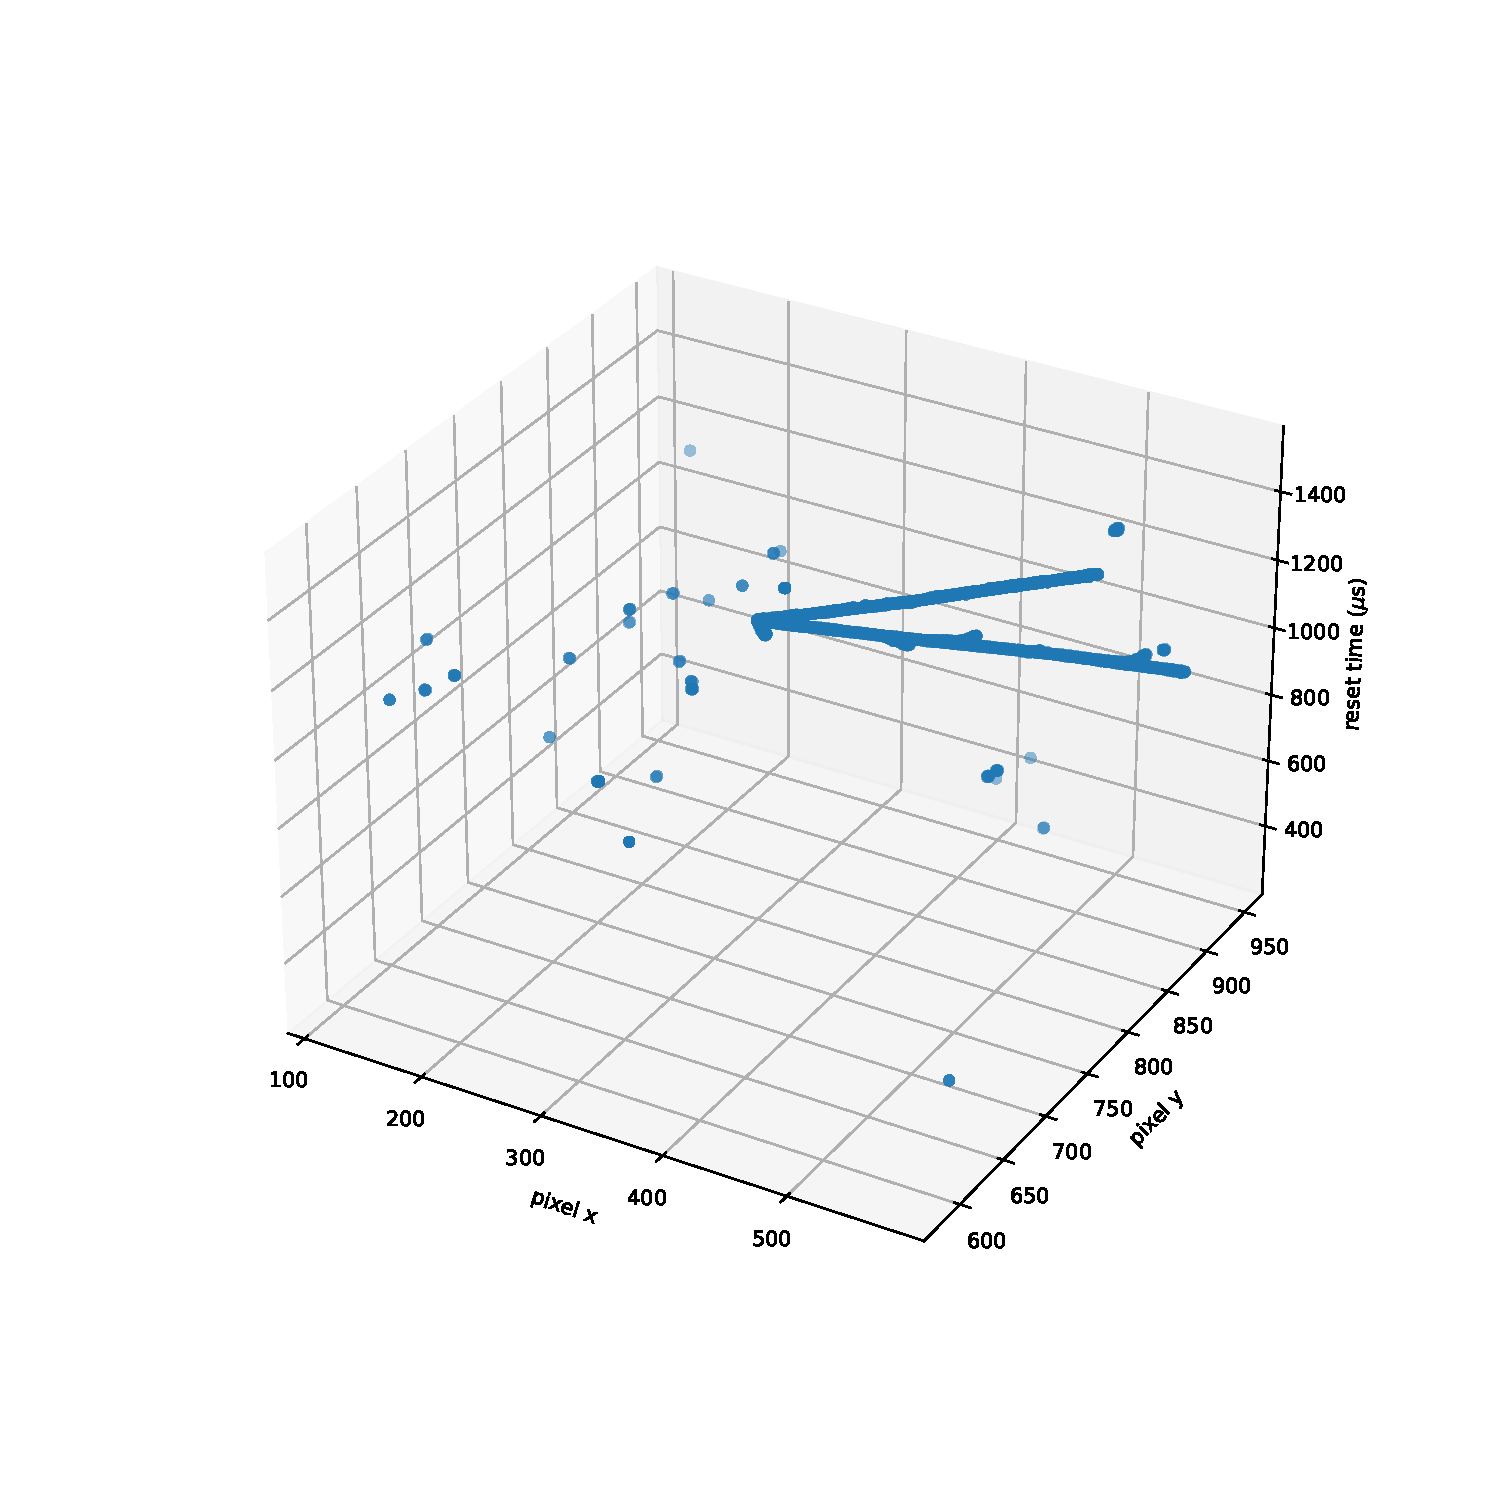
\includegraphics[width=\textwidth]{images/example_xdir_scatter.pdf}
  \caption{$\theta_{z} = 0$\unit{\degree}}
\end{subfigure}
\caption{Same $\nu_{e}$ interaction at Z-position $= 180 cm$, which is in the middle of the drift length of the APA.
Image (A) has the incident $\nu_{e}$ momentum rotated upwards ($\theta_{z} = +90$\unit{\degree}).
Image (B) has the incident $\nu_{e}$ had momentum along the beam direction ($\theta_{z} = 0$\unit{\degree})y.
Since there are five different z-positions, and five different $\theta_{z}$ values, each of the 3900 $\nu_{l}$ interactions are repeated 25 times.
These two plots show two of those 25 examples.
}
\label{fig:compare_integral}
\end{figure}

\begin{figure}[]
\centering
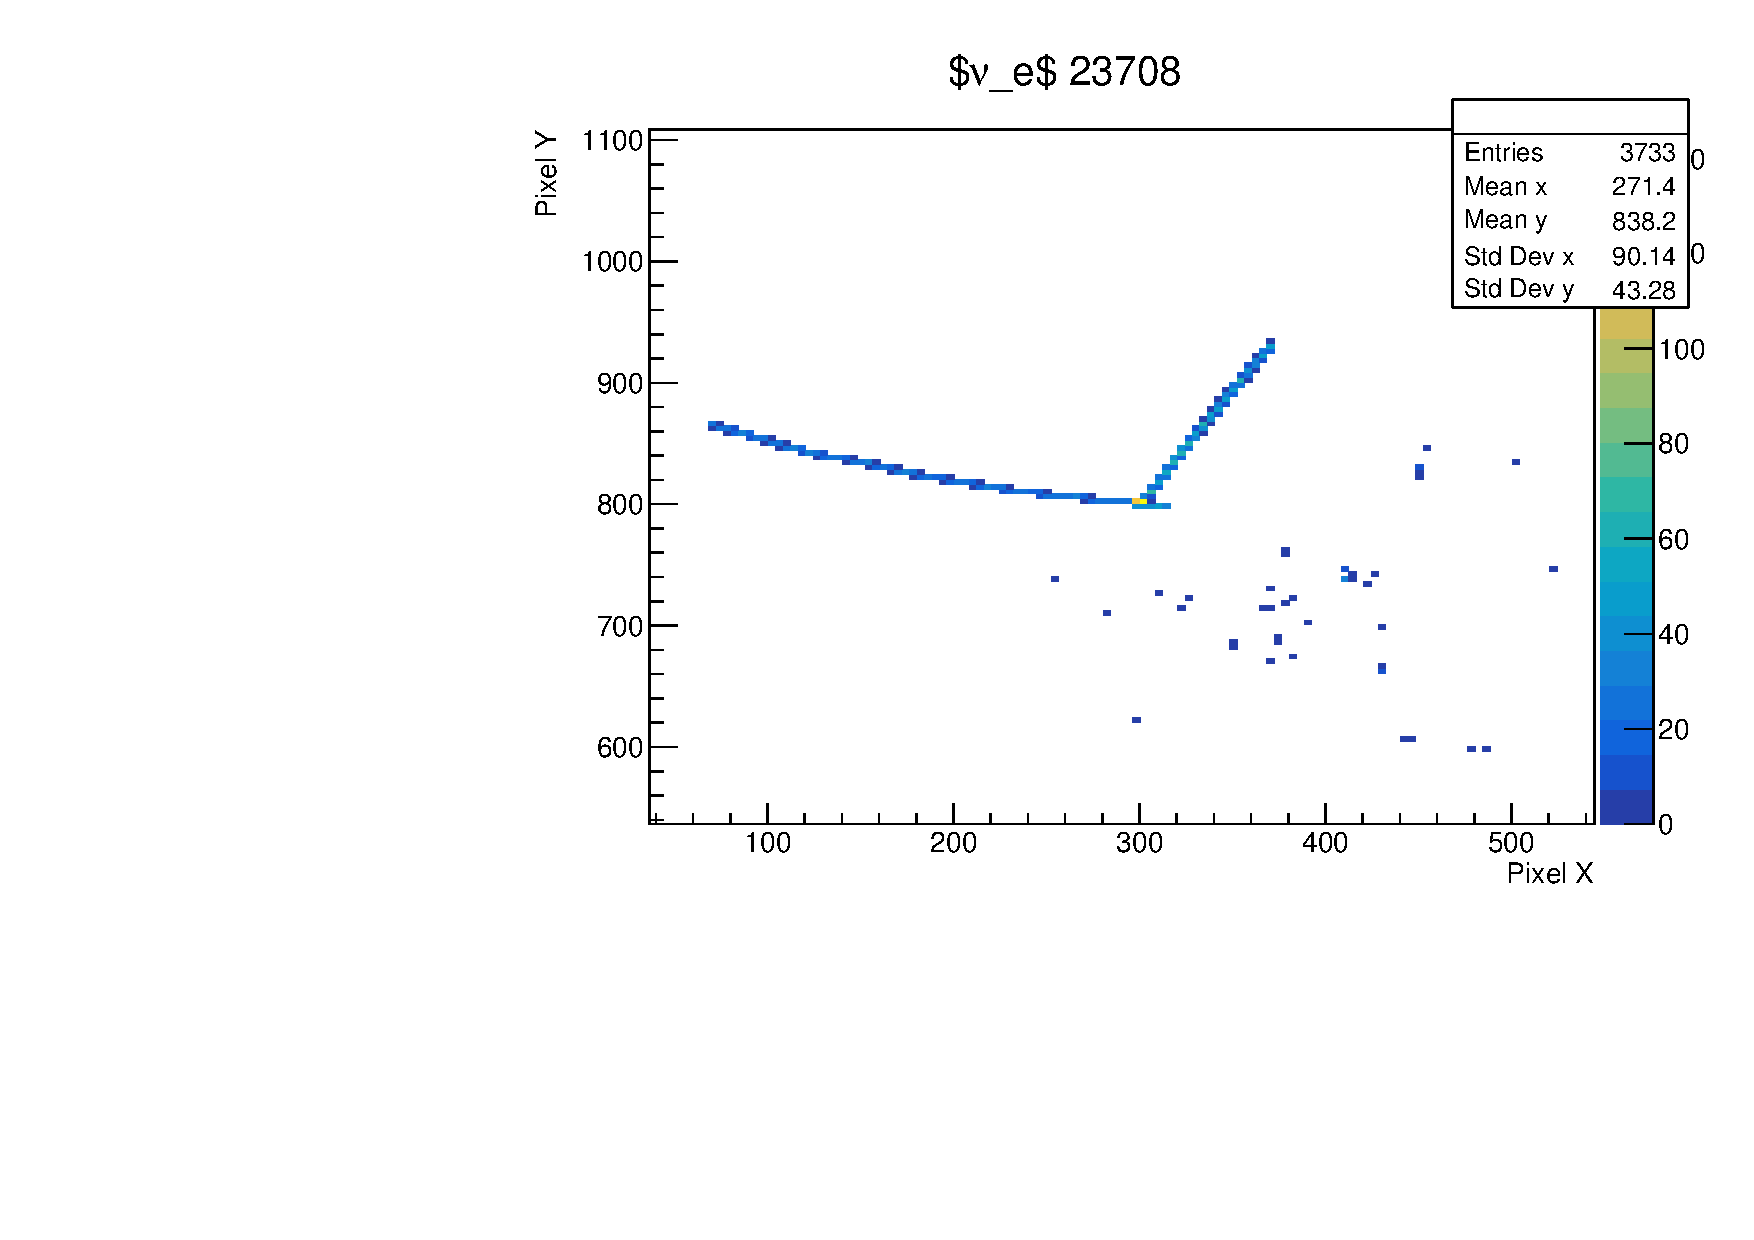
\includegraphics[width=\textwidth]{images/electron_fhc_23708_event.pdf}
\caption{The same $\nu_{e}$ event as the one shown in Figure~\ref{fig:compare_integral}-(A).
The plot is zoomed into to the region of interest where the bin widths represent the pixels dimensions in the collection plane.
The energy of this $\nu_{e}$ was 546.1~\unit{MeV}, and considering that each reset requires 0.1475~\unit{MeV}, the maximum number of resets this event could produce is $\approx 4368$.
The histogram records 3733 total resets.
The most active pixel received 144 resets.
When the pixels are binned into ASICs (4$\times$4 pixels) the maximum number resets an ASIC received is 347.
}
\end{figure}~\label{fig:asic_th2i_electron_fhc_event}

\subsection{Neutrino Event Results}

Every simulated neutrino interaction generates some number of resets which are collected onto the pixel plane.
The purpose of the study explored by the parameters described in Table~\ref{table:neutrino_params} is to investigate the charge resets these interactions produce; we pay particularly close attention to ASICs where the number of resets (energy deposited) is the largest in a given event.

We bin the maxmimum number of resets in a 4$\times$4 pixel array, or ASIC, for every neutrino event.
The plot Figure~\ref{fig:example_asic_integral_value_constTheta}-(A) shows a $\nu_{e}$ event and Figure~\ref{fig:asic_th2i_electron_fhc_event} shows these resets binned into pixels.
For every event we take the maximum ASIC value and use that as an entry into a histogram.
Next, we take the integral of each histogram as shown in (B) of Figure~\ref{fig:example_asic_integral_value_constTheta} and (B) of Figure~\ref{fig:example_asic_integral_value_constZpos}.
The value of this integral gives the percentage of fully events a function of local FIFO depth.

%% example integral of ASIC buffer depths with constant theta
\begin{figure}
\centering
\begin{subfigure}{.5\textwidth}
  \centering
  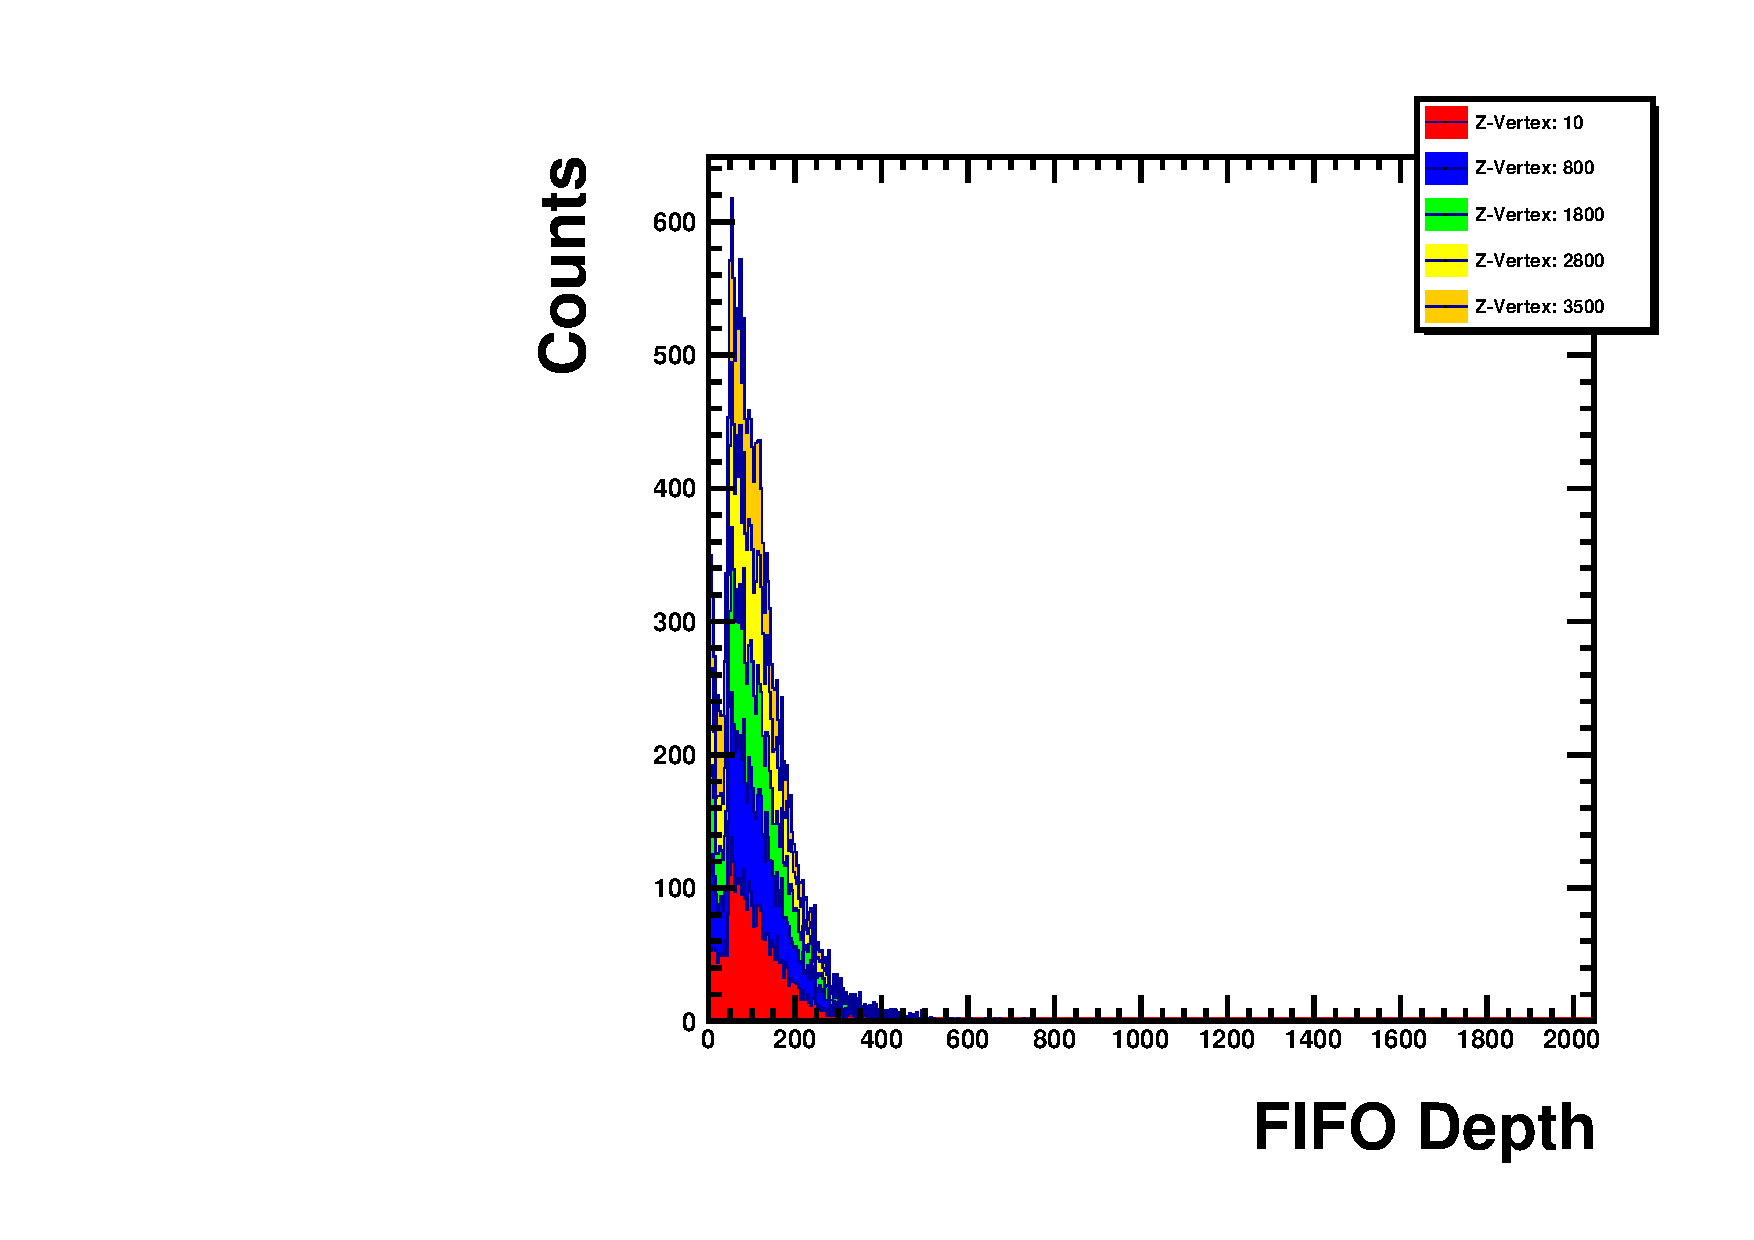
\includegraphics[width=\textwidth]{images/Const_Theta0_ASIC_stack_integral_pdg12_fhc.pdf}
  \caption{ASIC Local FIFO Depths}
\end{subfigure}%
\begin{subfigure}{.5\textwidth}
  \centering
  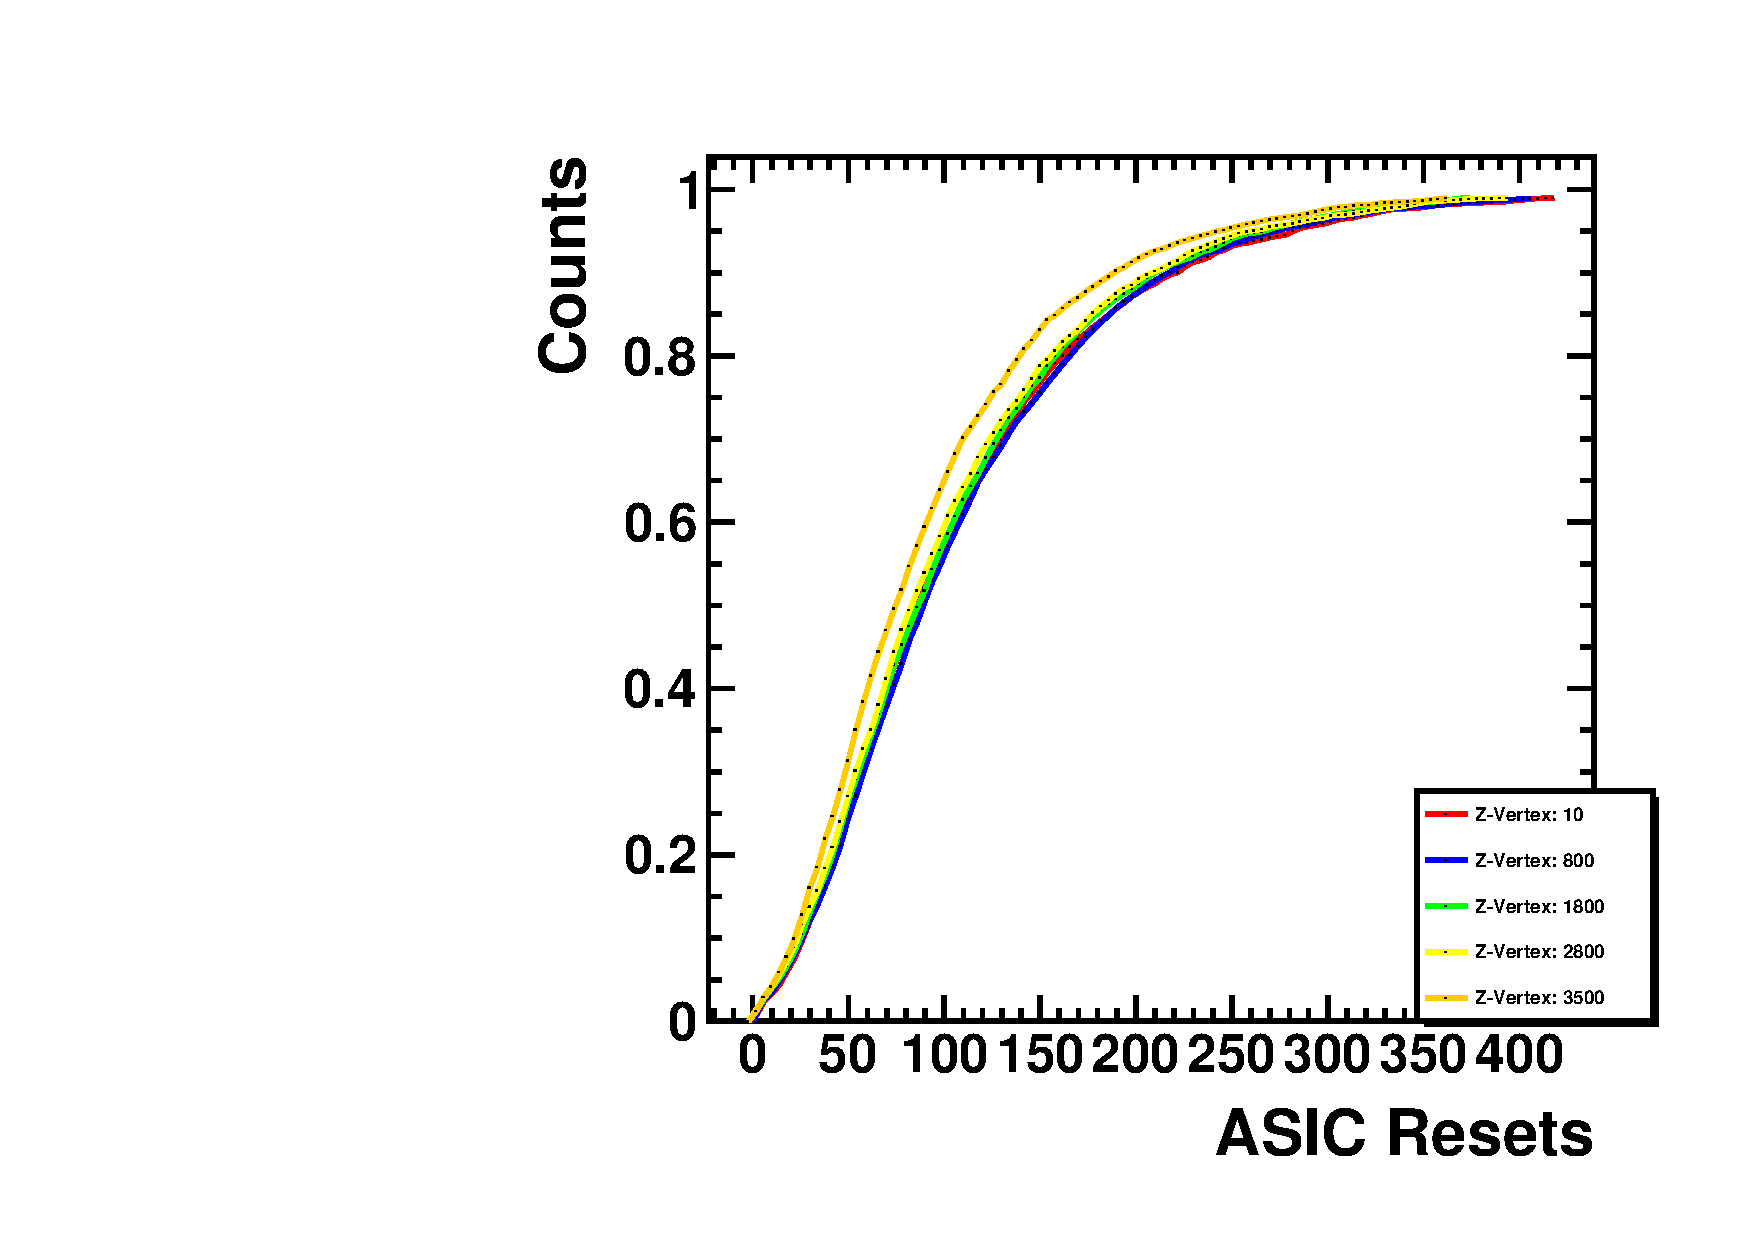
\includegraphics[width=\textwidth]{images/Const_Theta0_ASIC_integral_pdg12_fhc.pdf}
  \caption{Integral of FIFO depths}
\end{subfigure}
\caption{Example $\nu_{e}$ events for different z-position of the vertex with $\theta_{z} = 0$ held constant.
Plot (A) bins the maximum value of local FIFO depth for all 3900 events ($\nu_{l}$ energies between 250~\unit{MeV} - 10~\unit{GeV}) for variable z-position and $\theta_{z} = 0$.
Plot (B) shows the running integral for each histogram shown in plot (A).
The integral continues until 99\% of all events are counted.
This process is repeated for all 200 possible parameter choices as discussed in Table~\ref{table:neutrino_params}.
}
\label{fig:example_asic_integral_value_constTheta}
\end{figure}

%% example integral of ASIC buffer depths with constant zpos value
\begin{figure}
\centering
\begin{subfigure}{.5\textwidth}
  \centering
  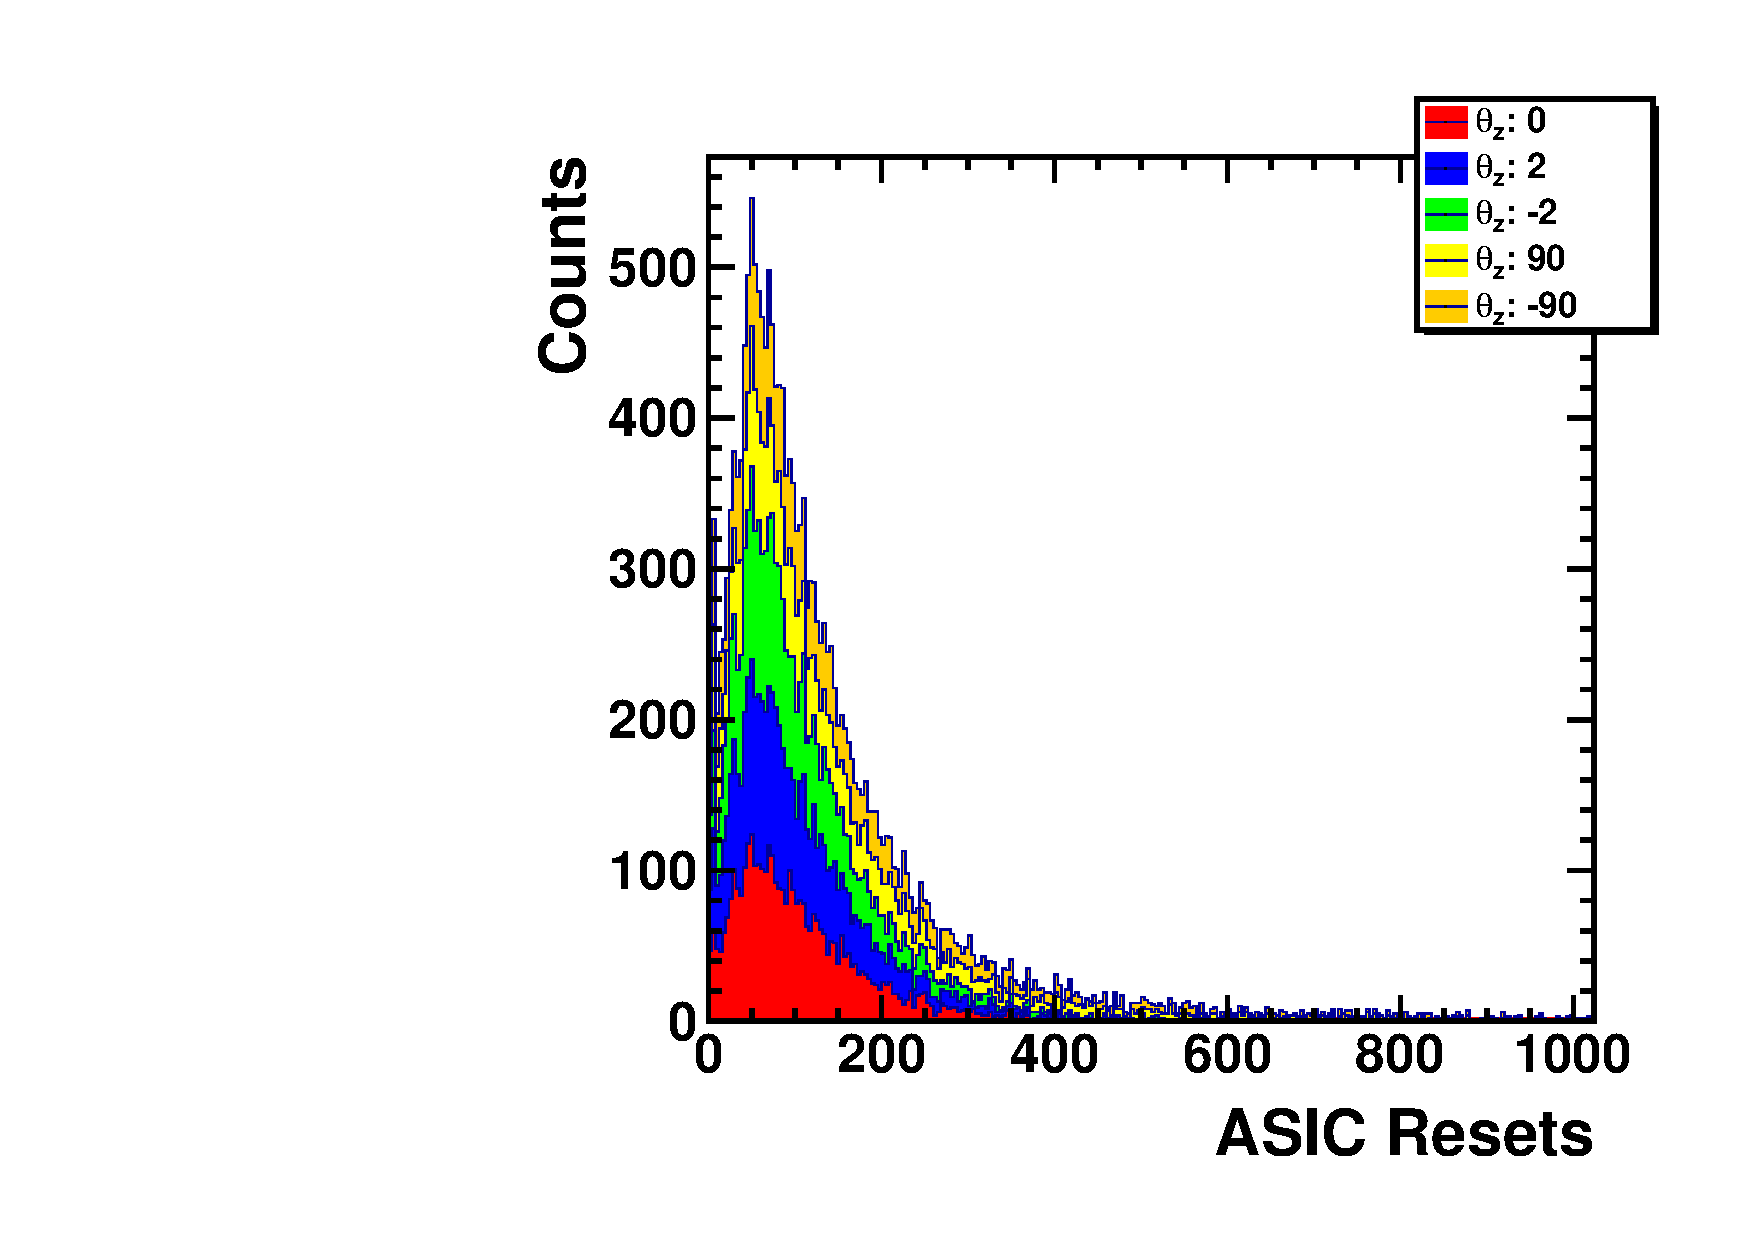
\includegraphics[width=\textwidth]{images/Const_Z180_ASIC_stack_integral_pdg12_fhc.pdf}
  \caption{ASIC Local FIFO Depths}
\end{subfigure}%
\begin{subfigure}{.5\textwidth}
  \centering
  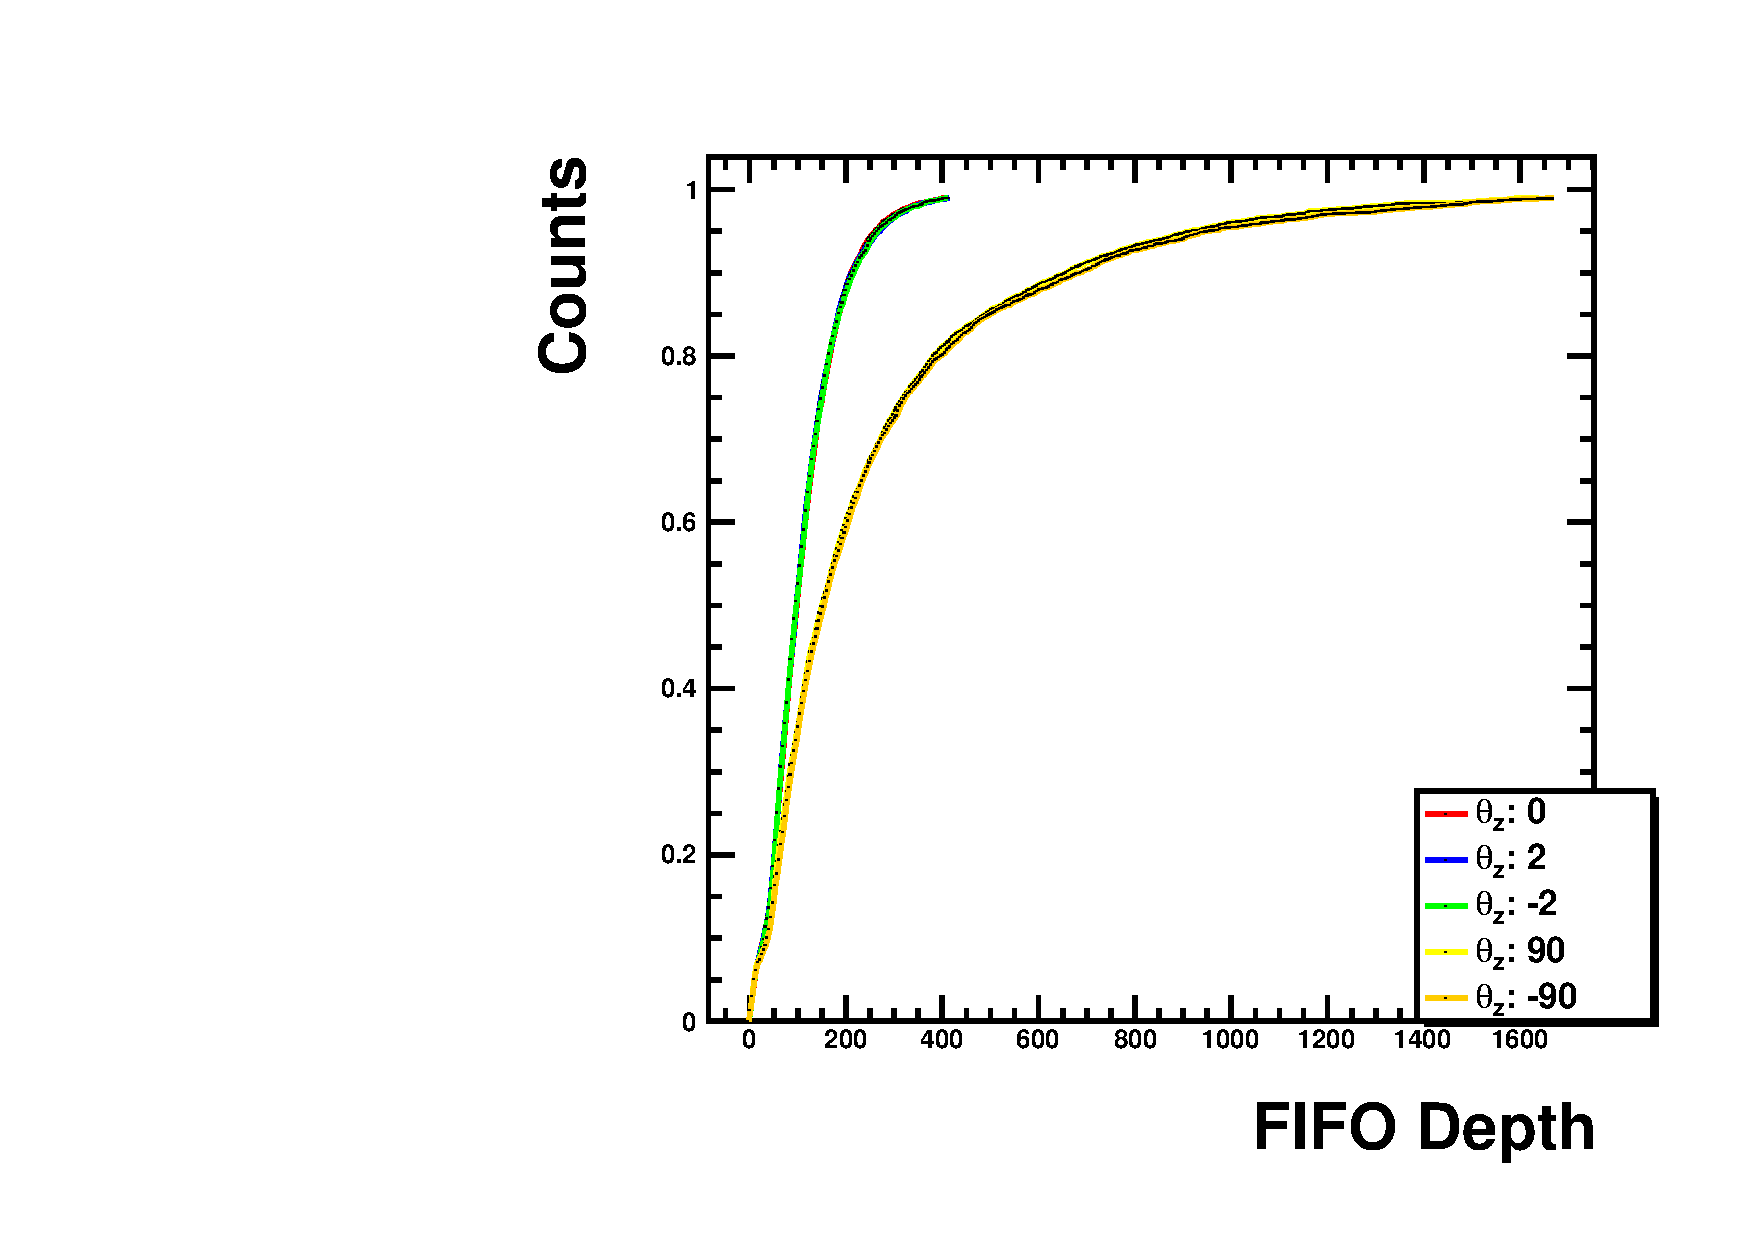
\includegraphics[width=\textwidth]{images/Const_Z180_ASIC_integral_pdg12_fhc.pdf}
  \caption{Integral of FIFO depths}
\end{subfigure}
\caption{Example $\nu_{e}$ events for different $\theta_{z}$ with the vertex held constant with z-position = 180~\unit{cm}.
This is a similar plot to Figure~\ref{fig:example_asic_integral_value_constTheta} with the exception that $\theta_{z}$ is varied and the z-position is held constant at z = 180~\unit{cm}.
A notable difference to note here is the run away effect of the large values of $\theta_{z}$.
This effect is intuitive: the initial momentum direction affects the direction of where most charge will be deposited.
As more charge is localized an ASICs area, it will collect more resets. 
}
\label{fig:example_asic_integral_value_constZpos}
\end{figure}

\subsection{Neutrino Energy Deposit}

The true neutrino interaction energy is notoriously difficult to reconstruct.
The neutrino itself carries no charge and its track is not directly reconstructed in the LAr.
Other effects such as long neutron drift make perfect energy reconstruction of the neutrino interaction impossible by principle.
For these reasons we show how the resets and ASIC FIFO depths vary both by the energy deposited into the LAr as well as the true neutrino energy.
Figure~\ref{fig:example_asic_energy_comparison} shows the relationship between the true $\nu_{e}$ energy and the max FIFO depth as well as the total APA resets.
Figure~\ref{fig:compare_energy_deposit} shows the same relationships instead as a function of the energy deposited.

%% energy comparison for different different zpos and theta values
\begin{figure}
\centering
\begin{subfigure}{.5\textwidth}
  \centering
  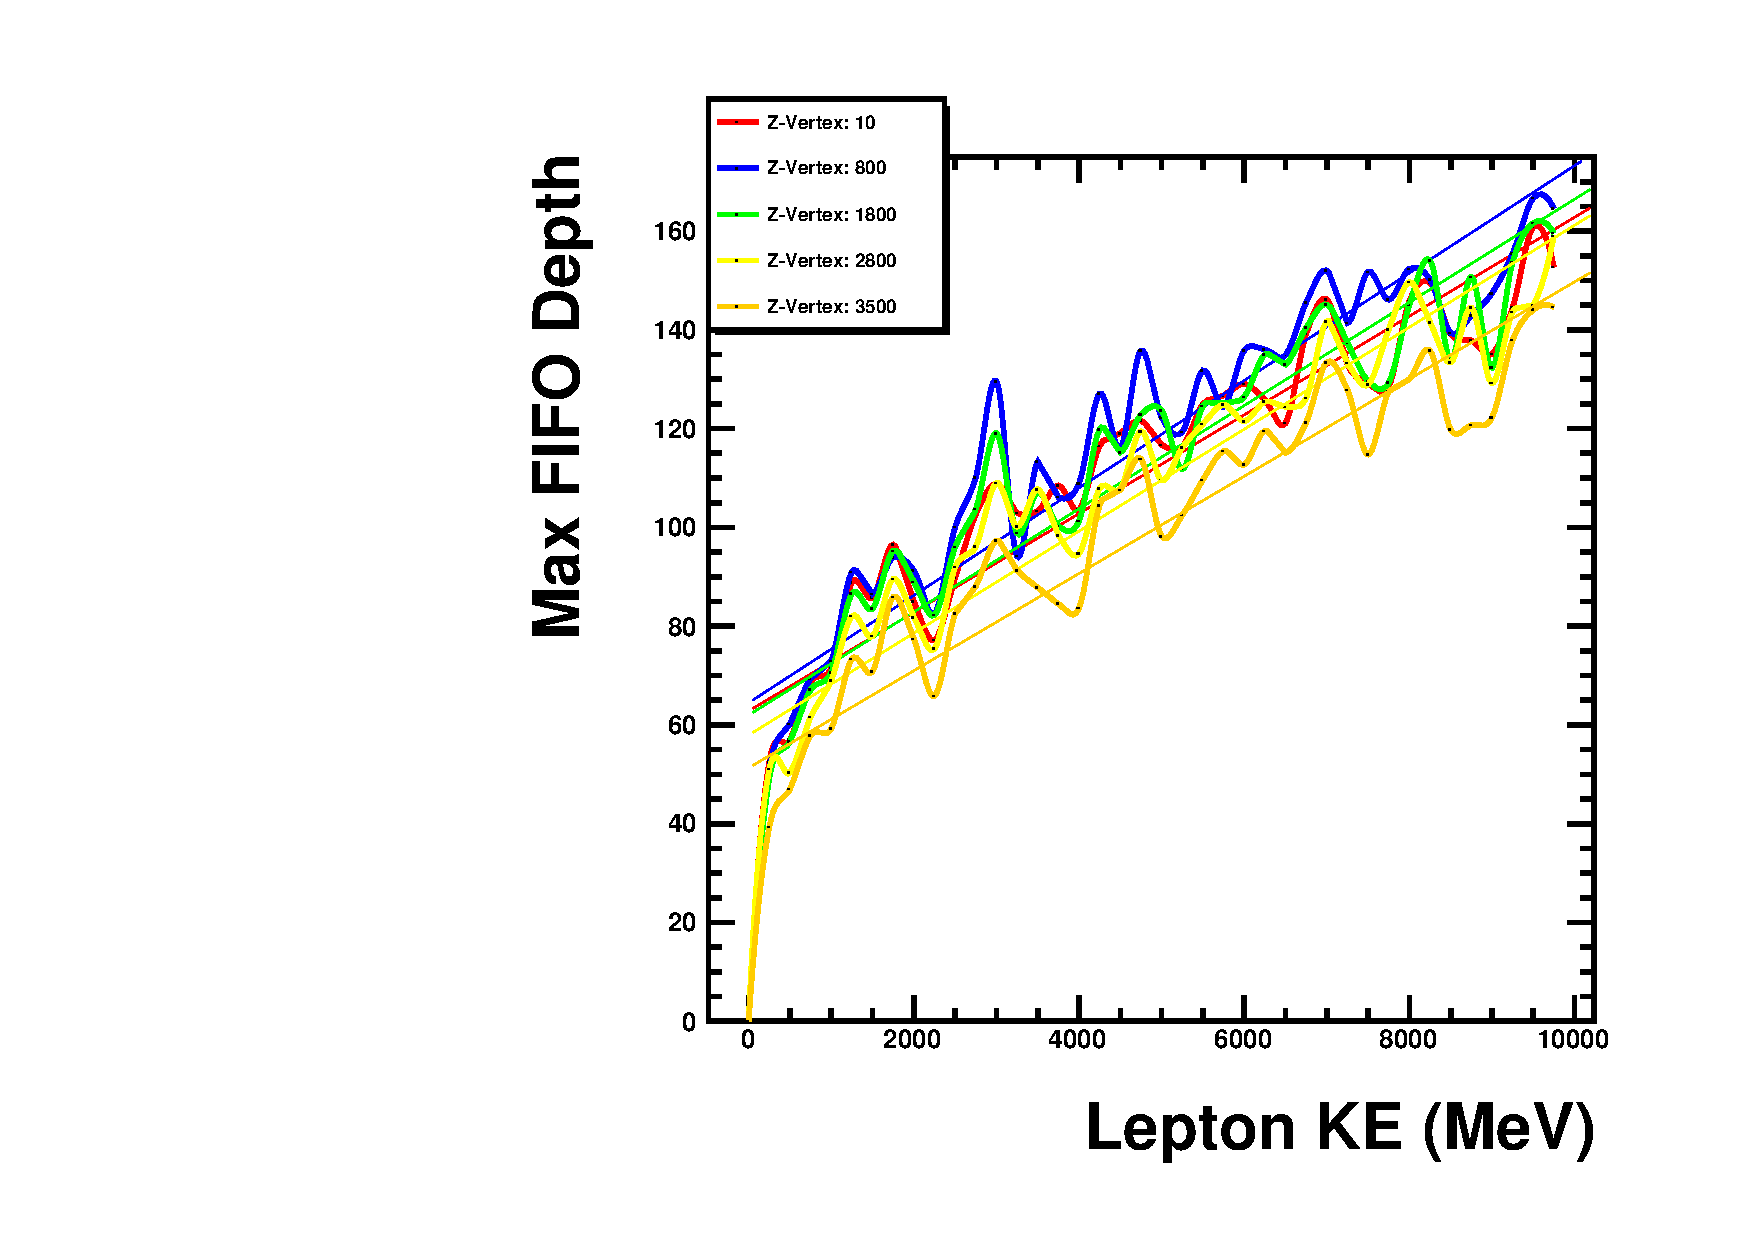
\includegraphics[width=\textwidth]{images/Const_Theta0_ASIC_lepKE_multigraph_pdg12_fhc.pdf}
  \caption{Constant $\theta_{z} = 0$ direction.}
\end{subfigure}%
\begin{subfigure}{.5\textwidth}
  \centering
  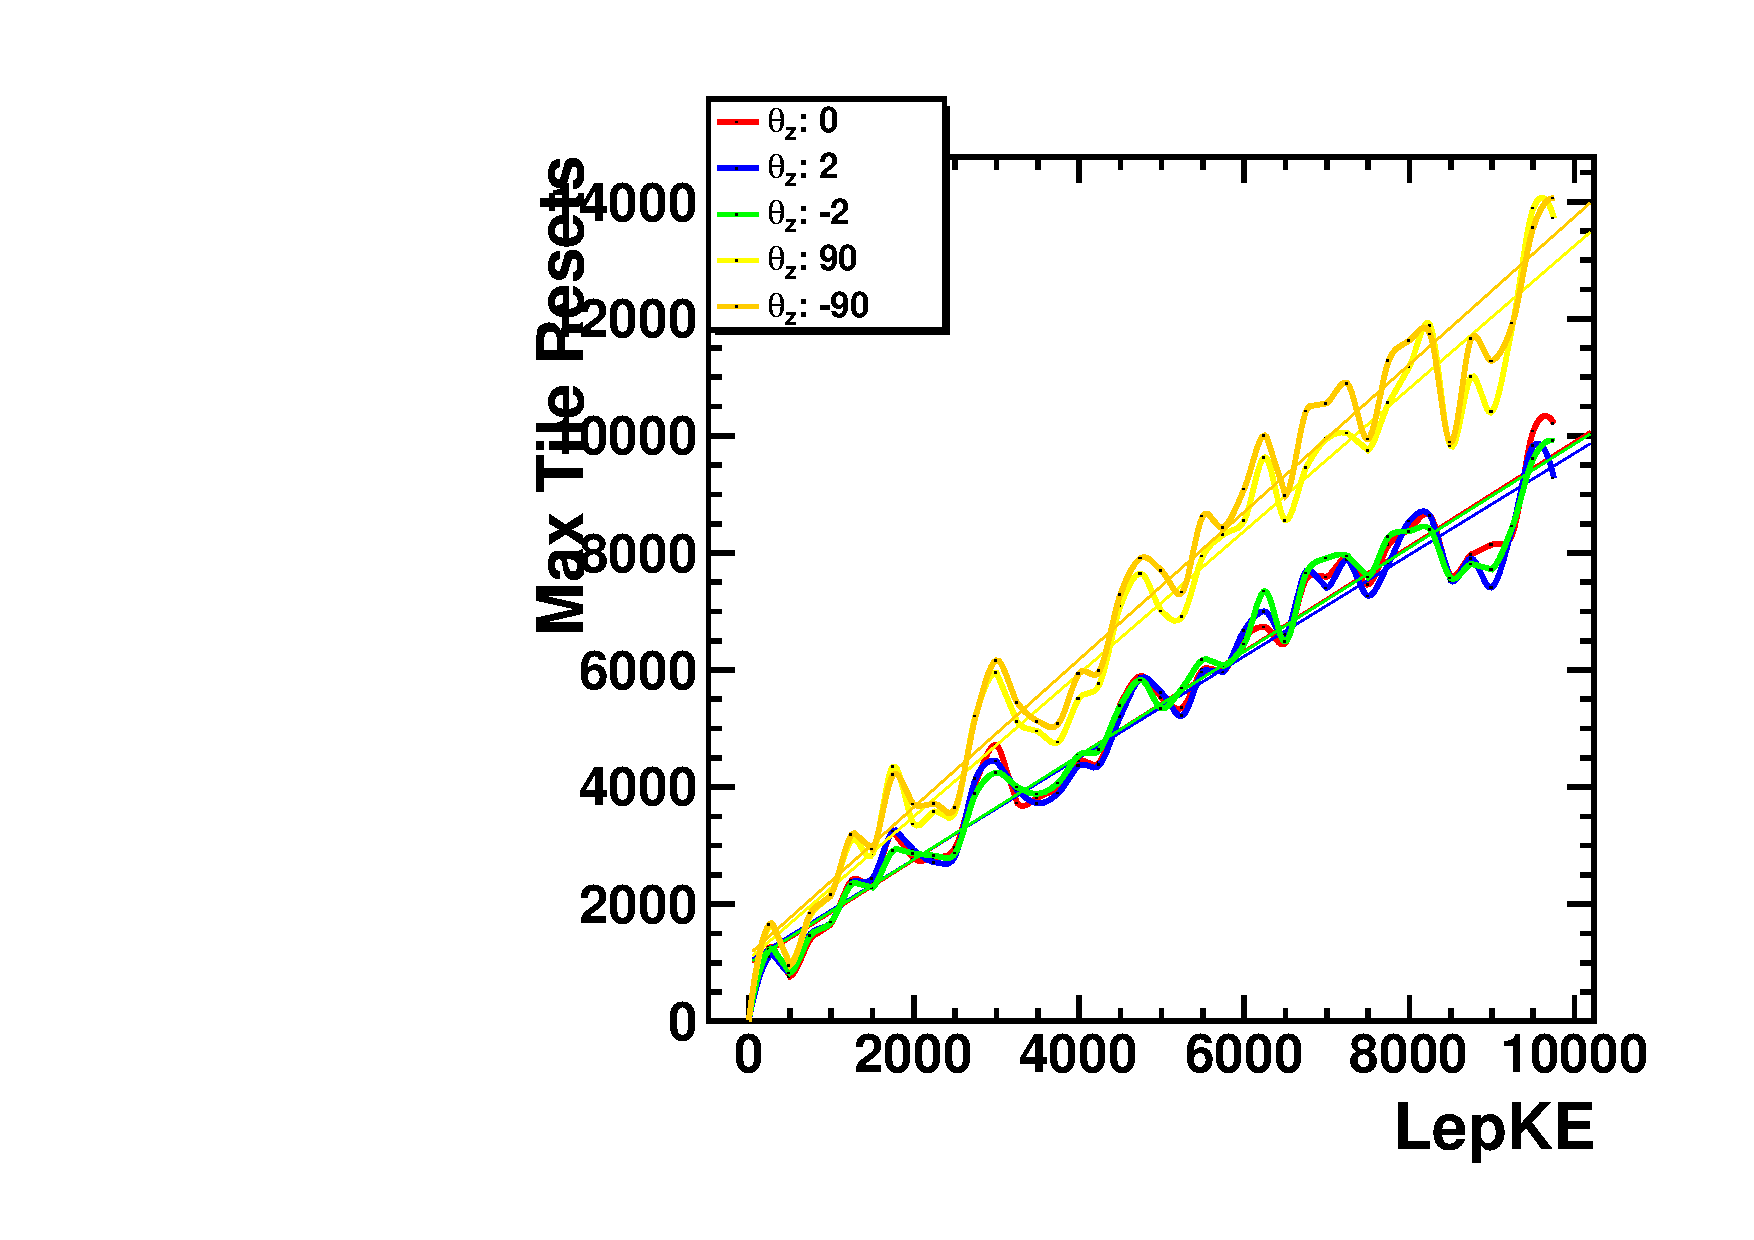
\includegraphics[width=\textwidth]{images/Const_Z180_ASIC_lepKE_multigraph_pdg12_fhc.pdf}
  \caption{Constant Z-Position: $Z = 180~$\unit{cm}.}
\end{subfigure}
\caption{Comparison of Buffer depths as a function of energy for different parameters of $\theta_{z}$ and z-position.
There is a large variance between the true $\nu_{l}$ incident energy and the actual energy deposited in the LAr.
This is the reason why only the means are plotted for each energy bin.
}
\label{fig:example_asic_energy_comparison}
\end{figure}

%% compare energy deposit and lepton energy
\begin{figure}
\centering
\begin{subfigure}{.5\textwidth}
  \centering
  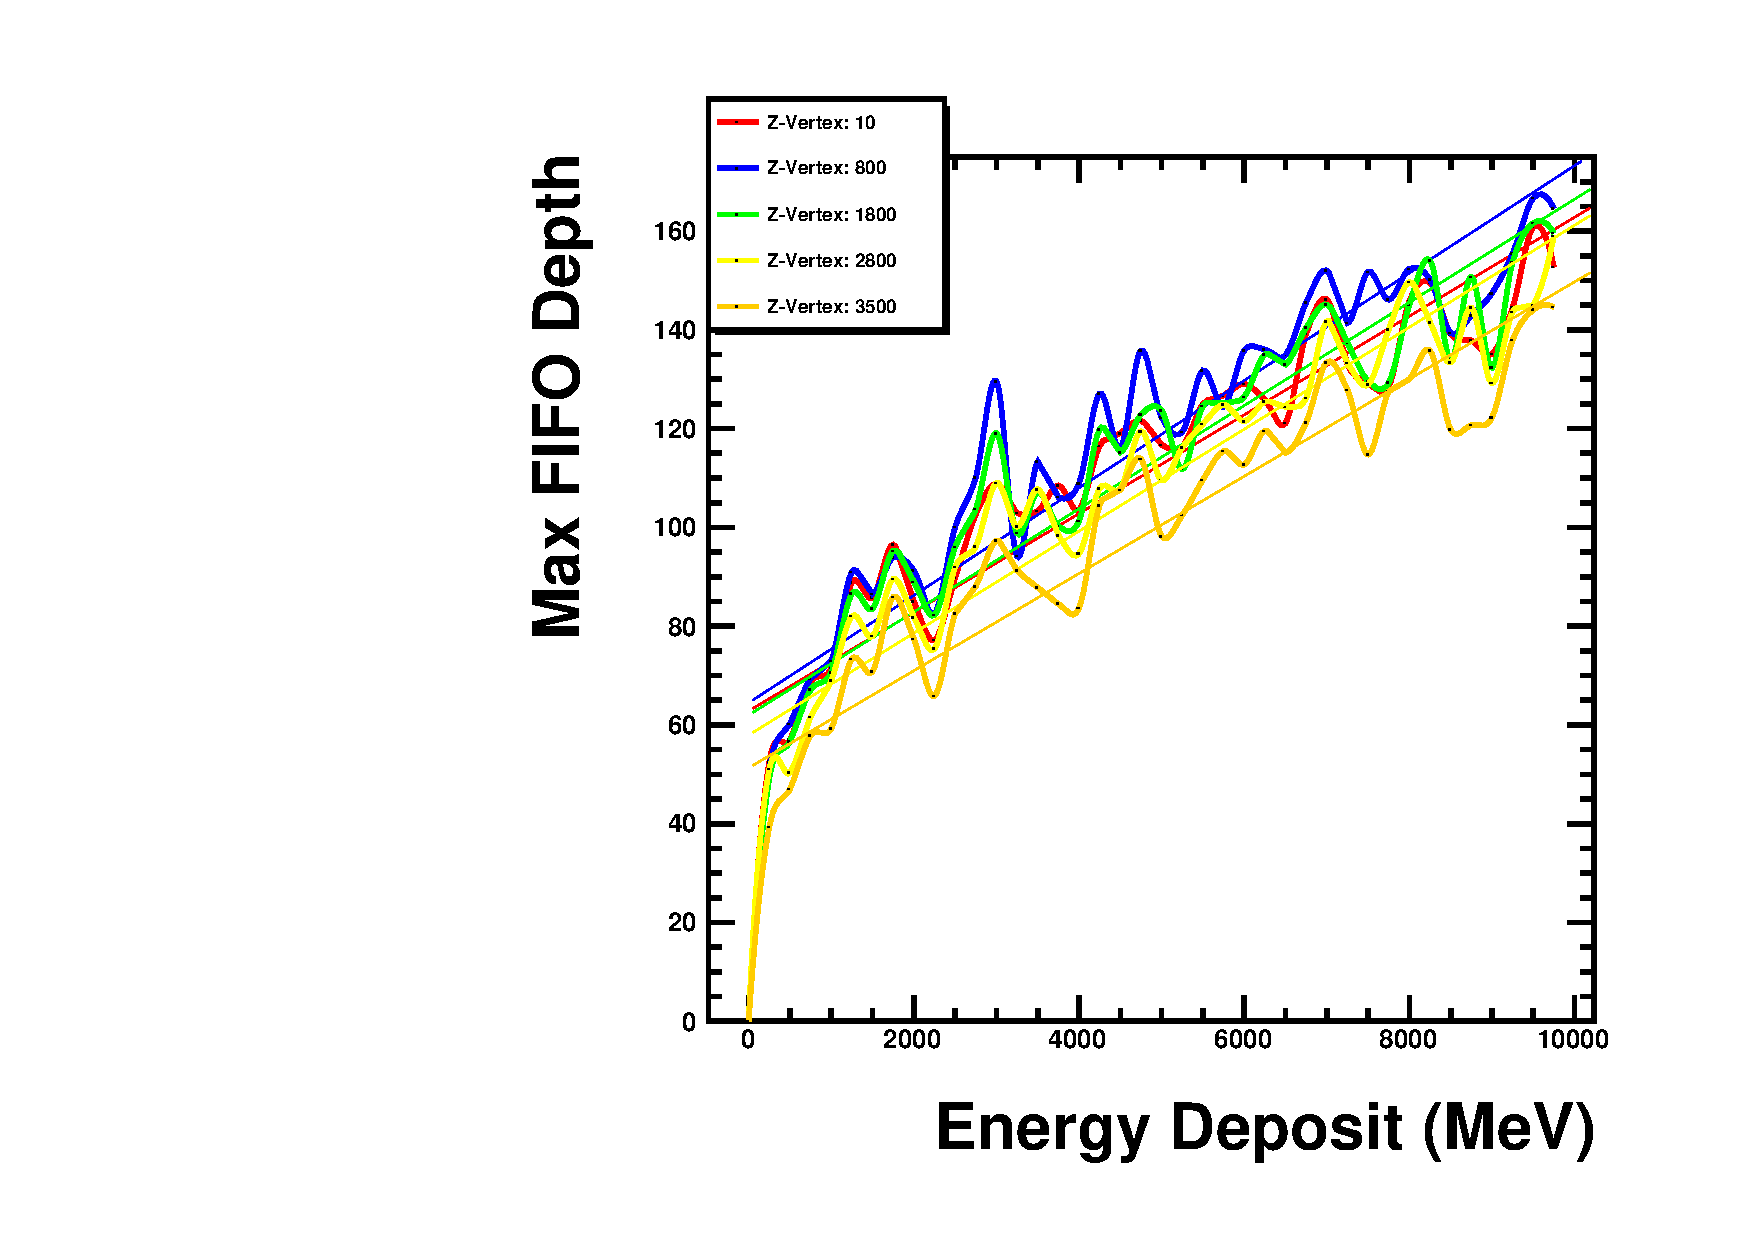
\includegraphics[width=\textwidth]{images/Const_Theta0_ASIC_EnergyDep_multigraph_pdg12_fhc.pdf}
  \caption{}
\end{subfigure}%
\begin{subfigure}{.5\textwidth}
  \centering
  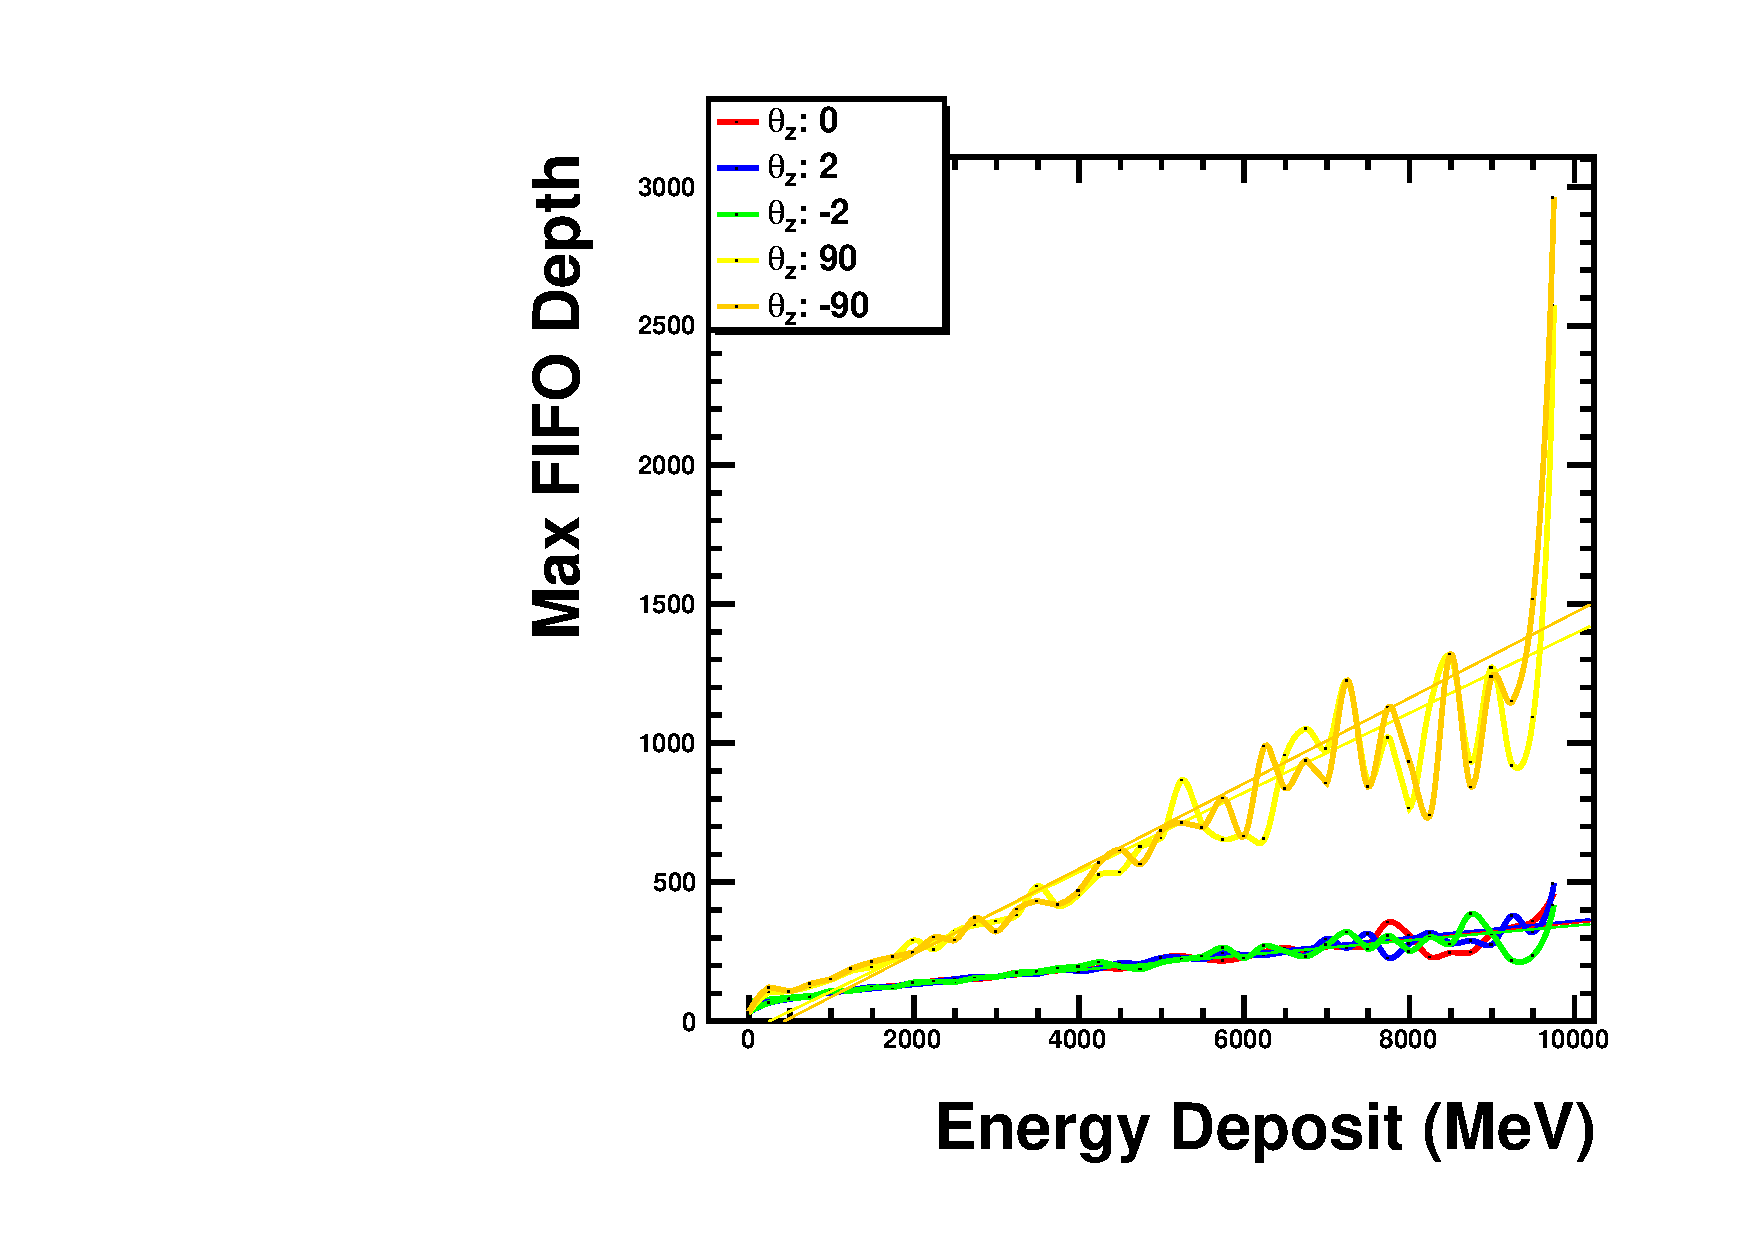
\includegraphics[width=\textwidth]{images/Const_Z180_ASIC_EnergyDep_multigraph_pdg12_fhc.pdf}
  \caption{}
\end{subfigure}
\caption{A comparison of ASIC resets vs the energy deposited into the LAr.
Plot-(B) shows for Z-position=10~\unit{cm} ends at $\approx$ 2~\unit{GeV} since no $\nu_{e}$ events deposit this much energy into the LAr.
Both plots indicate that the 
}
\label{fig:compare_energy_deposit}
\end{figure}

One of the key differences of a Q-Pix readout compared to a traditional waveform readout is that the amount of data the Q-Pix readout collects depends on the energy deposited.
Since Q-Pix is fundamentally a counting readout, the amount of counts (data) it collects depends on the amount of energy deposited.
Therefore, one limit on its bandwidth is the total amount of resets it can measure, which is proportional to the energy deposited as shown in Figure~\ref{fig:energy_deposit_vs_resets}.

%% compare energy deposit and lepton energy
\begin{figure}
\centering
\begin{subfigure}{.5\textwidth}
  \centering
  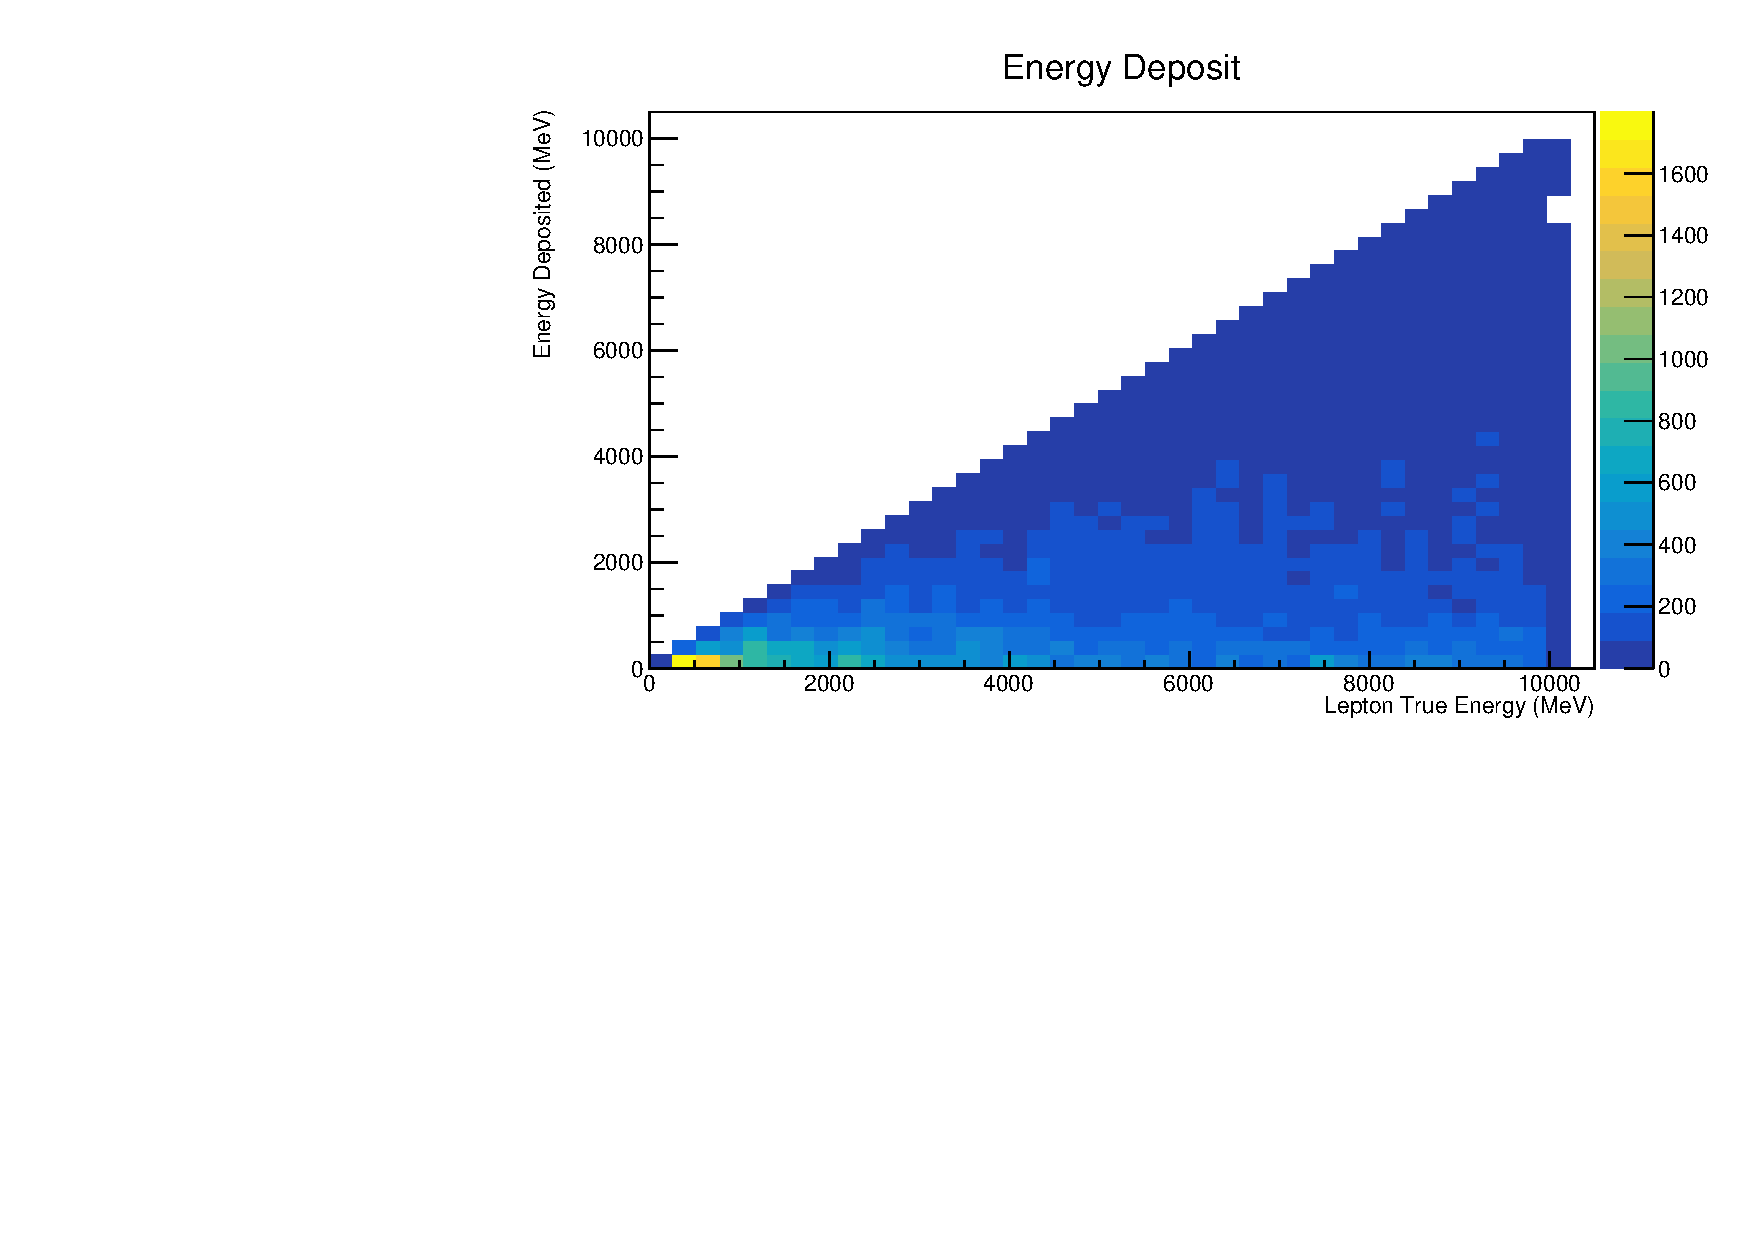
\includegraphics[width=\textwidth]{images/electron_nu_energy_deposit.pdf}
  \caption{}
\end{subfigure}%
\begin{subfigure}{.5\textwidth}
  \centering
  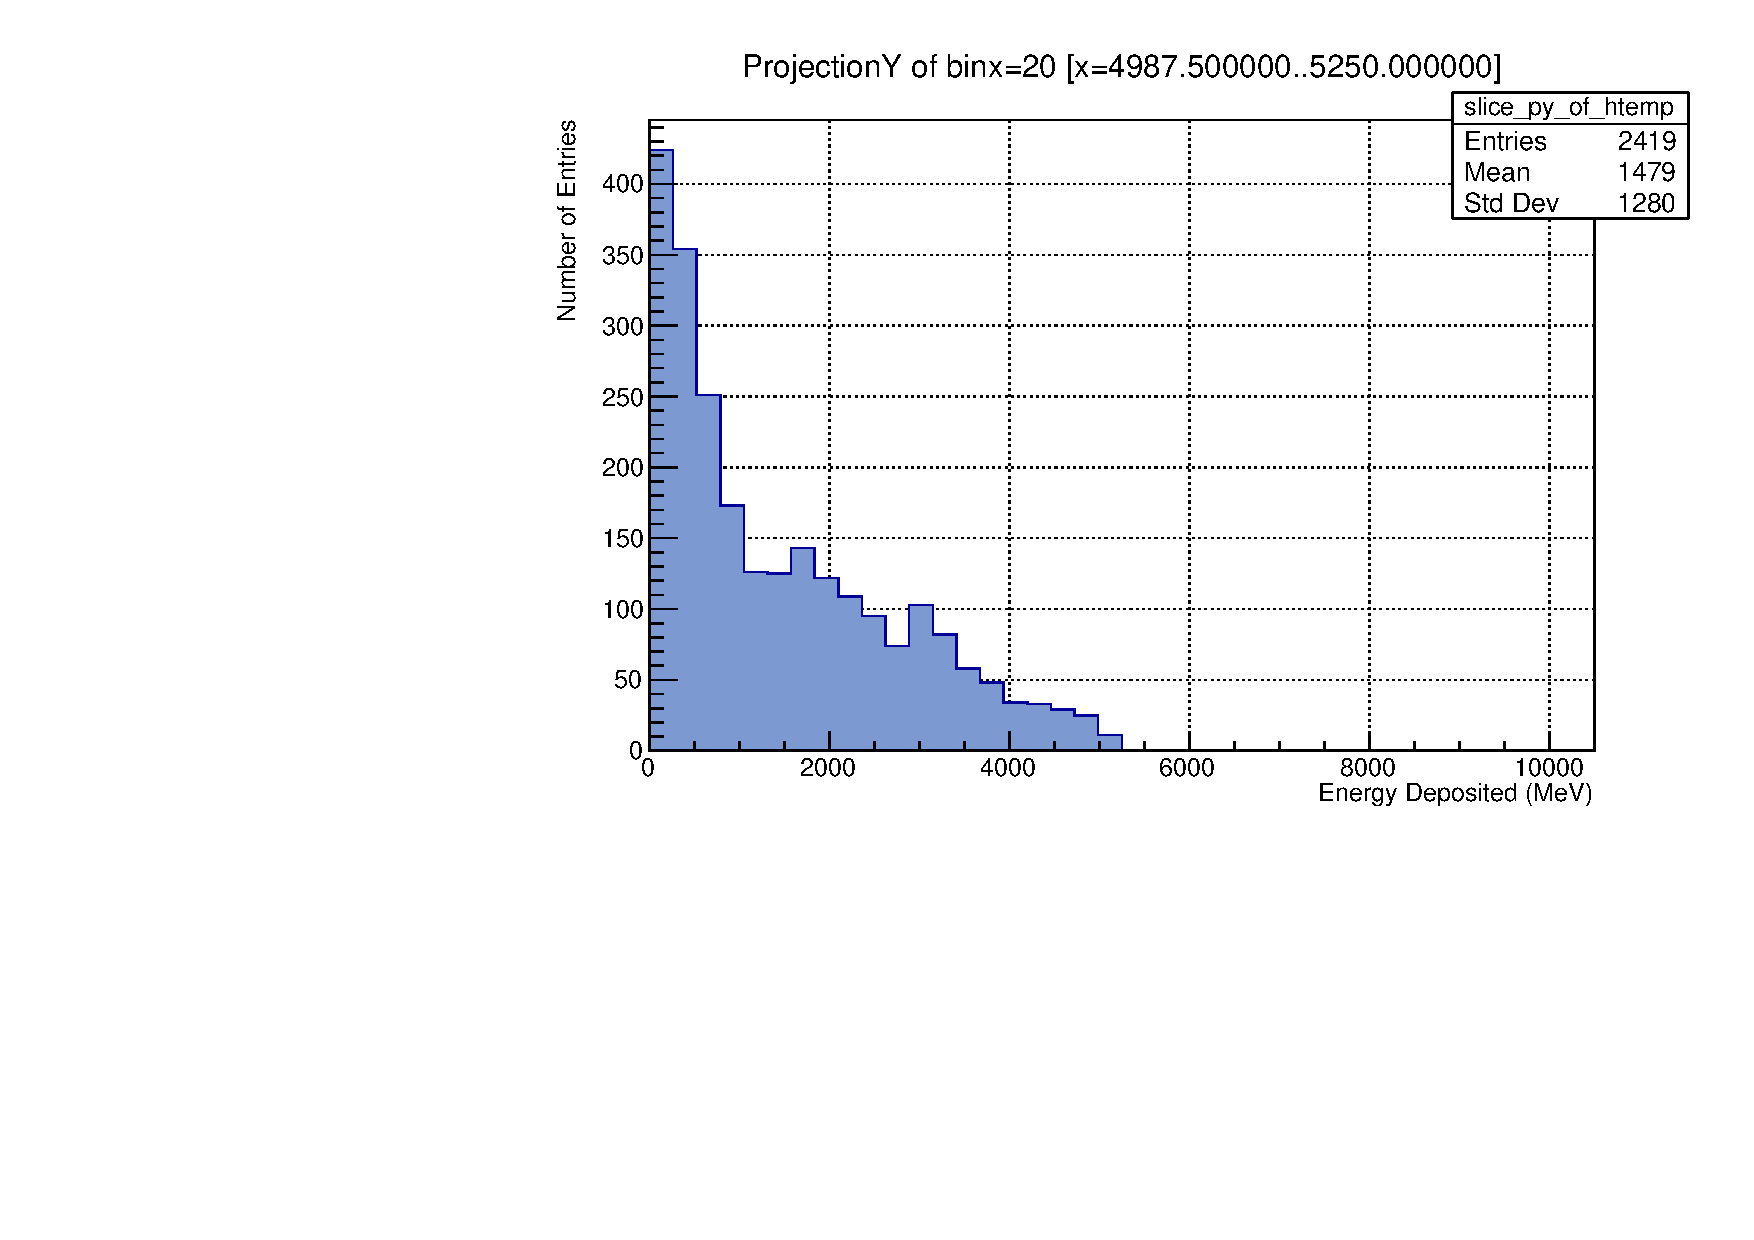
\includegraphics[width=\textwidth]{images/electron_nu_energy_deposit_slice.pdf}
  \caption{}
\end{subfigure}
\caption{Plot-(A) shows a comparison of the energy deposited into the LAr as a function of the input neutrino ($\nu_{e}$).
Plot-(B) shows a projection against the y-axis for a single bin.
The maximum allowed total energy deposited is limited to the total energy of the input neutrino.
However, the lower bound for all energies is still, obviously, zero.
Therefore, as the input neutrino energy increases the upper bound also increases.
The mean value of Plot-(B) indicates that even for a maximum allowed total energy of 5~\unit{GeV} the mean (average) energy deposited per event is 1479~\unit{MeV}.
Most interactions deposit less than 2~\unit{GeV} into the LAr, as shown in Figure~\ref{fig:example_energy_deposit}.
Some pileup events are removed, see Figure~\ref{fig:energy_deposit_vs_resets}.
}
\label{fig:example_energy_deposit}
\end{figure}

\begin{figure}[]
\centering
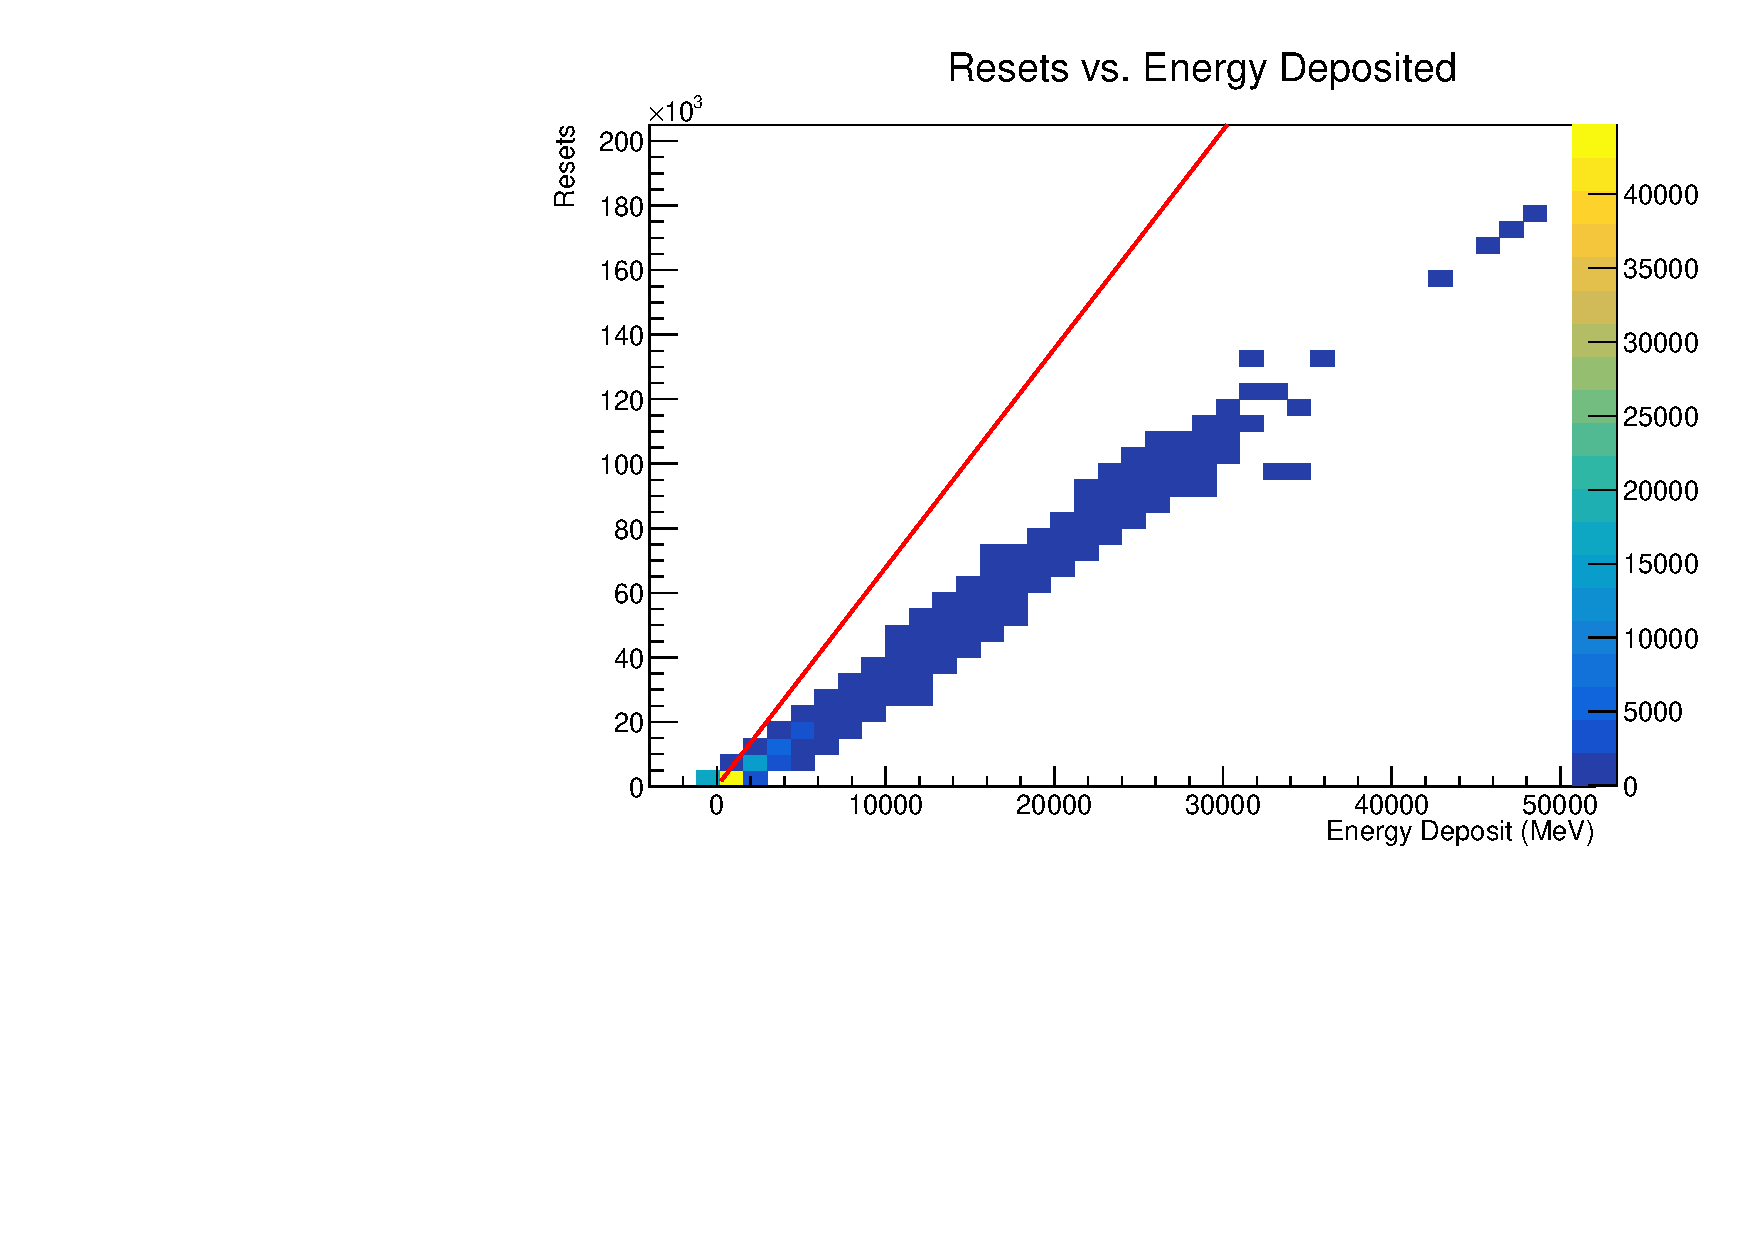
\includegraphics[width=\textwidth]{images/resets_vs_energy_deposit.pdf}
\caption{A relationship between the total number of resets detected in the APA and the energy deposited for $\nu_{e}$ interactions is shown.
The solid red line indicates the maximum number of resets that could be measured for a given energy.
The small distribution of energies below zero correspond to events that produced no resets.
The energy deposited goes above the the threshold limit of 10~\unit{GeV}.
These events carry extra energy from additional leptons which are from pile-up at the DUNE-ND from the FNAL beam.
These data are not included in the energy deposited analysis, or in the integrals as shown in Figure~\ref{fig:compare_integral}.
These high energy deposit events are also not included in the FIFO depth analysis, since these events are beyond the energy range for oscillation measurements.
These events are also removed from Figure~\ref{fig:example_energy_deposit}.
}
\end{figure}~\label{fig:energy_deposit_vs_resets}

\subsection{Local FIFO Depth Results}

To predict the required local FIFO depth for the Q-pix ASIC, we perform the intergral as shown in Figure~\ref{fig:example_asic_integral_value_constTheta} for each of the parameters described in Table~\ref{table:neutrino_params}. 
Since there are 200 different parameters, there are 200 different integral values.

Figure~\ref{fig:compare_integral_zpos_theta} and Figure~\ref{fig:compare_integral_nolabel} show the same integral results, but with different labeling.
The results show two different distributions of buffer depths: those along the near-beam angle ($\theta_{z} \approx 0$\unit{\degree}) and near the azumithal angle ($\theta_{z} \approx \pm 90$\unit{\degree}). 
The Table~\ref{tab:apa_sum} shows the values for the required local FIFO depth for each combination of the 200 parameters for the 95\% and 99\% capture intervals.

%% comparing integral results here
\begin{figure}
\centering
\begin{subfigure}{.5\textwidth}
  \centering
  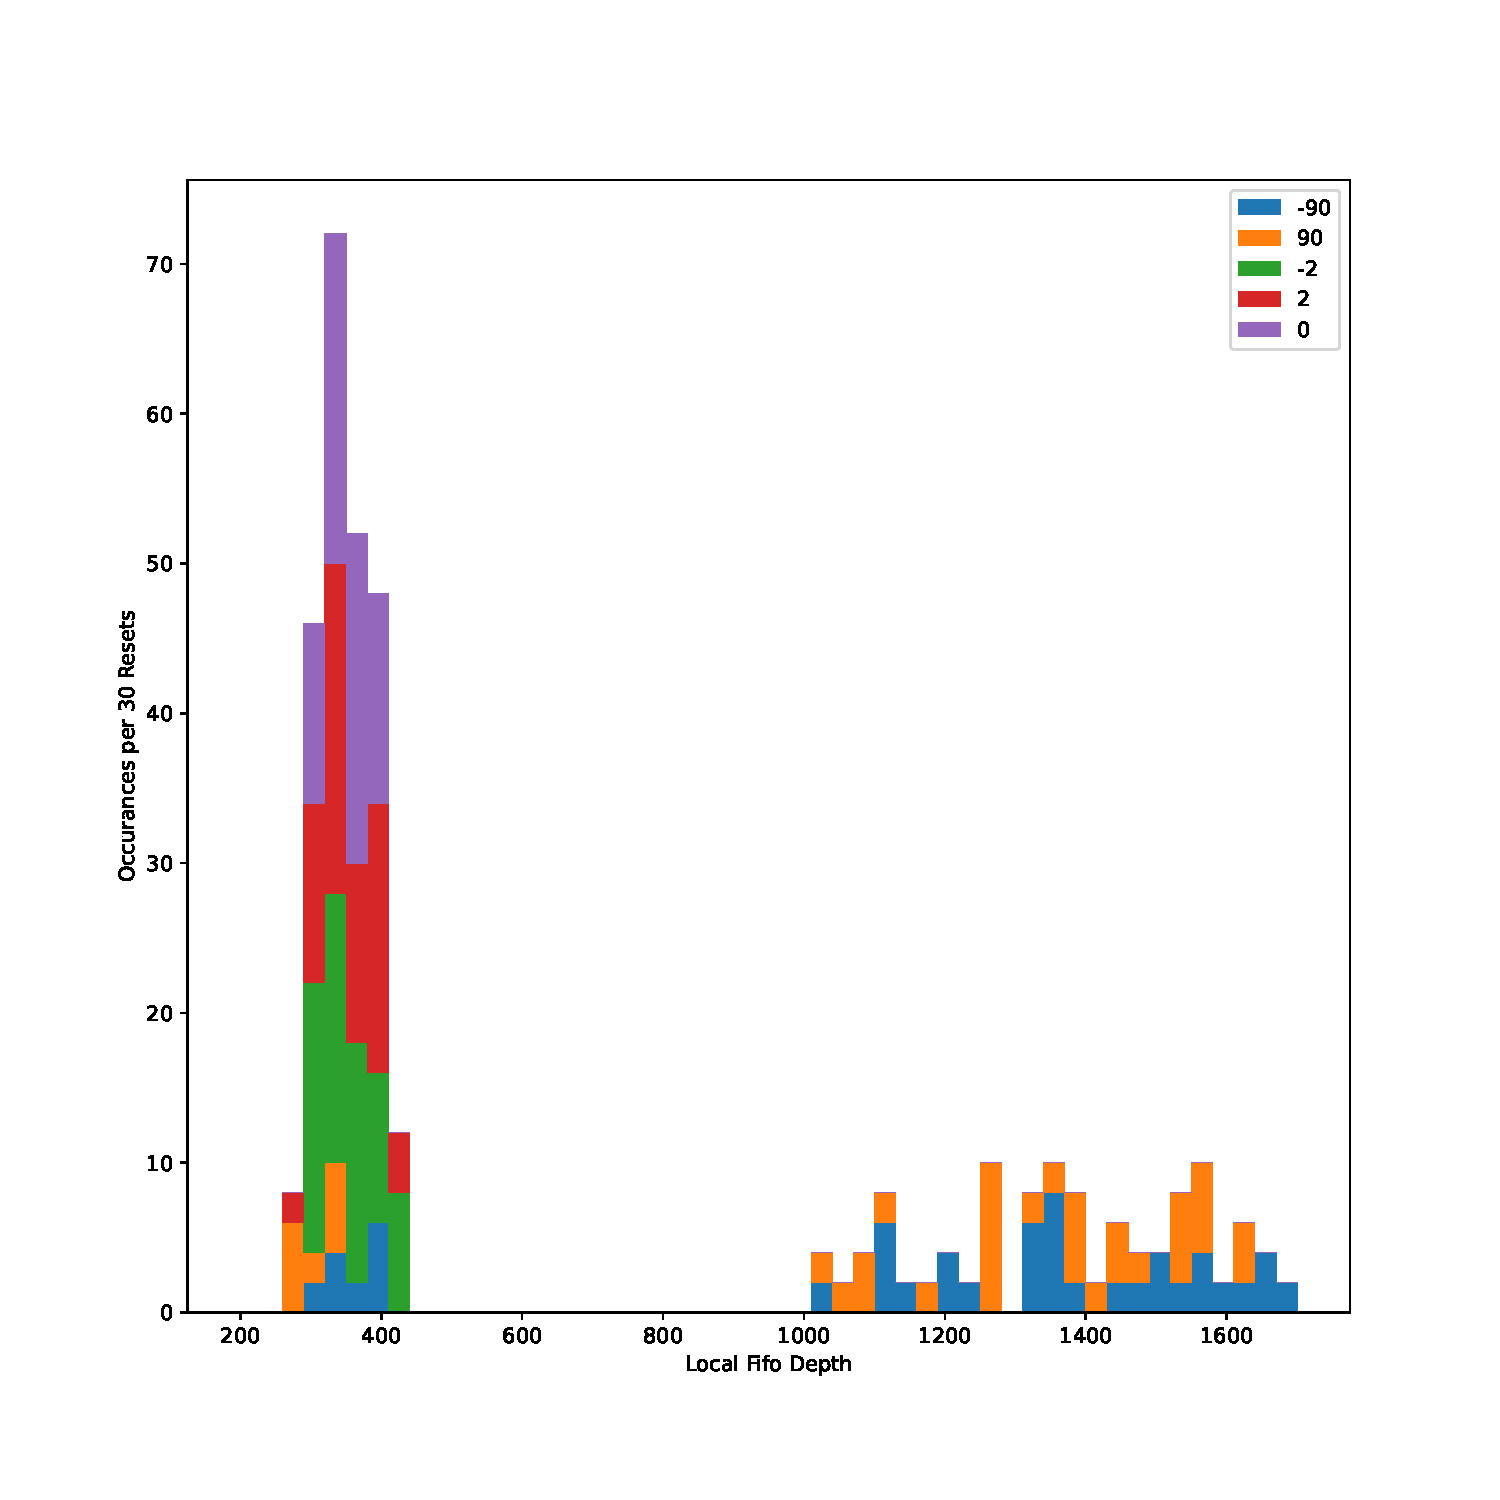
\includegraphics[width=\textwidth]{images/df_theta_cut.pdf}
  \caption{Colored by $\theta_{z}$ direction.}
\end{subfigure}%
\begin{subfigure}{.5\textwidth}
  \centering
  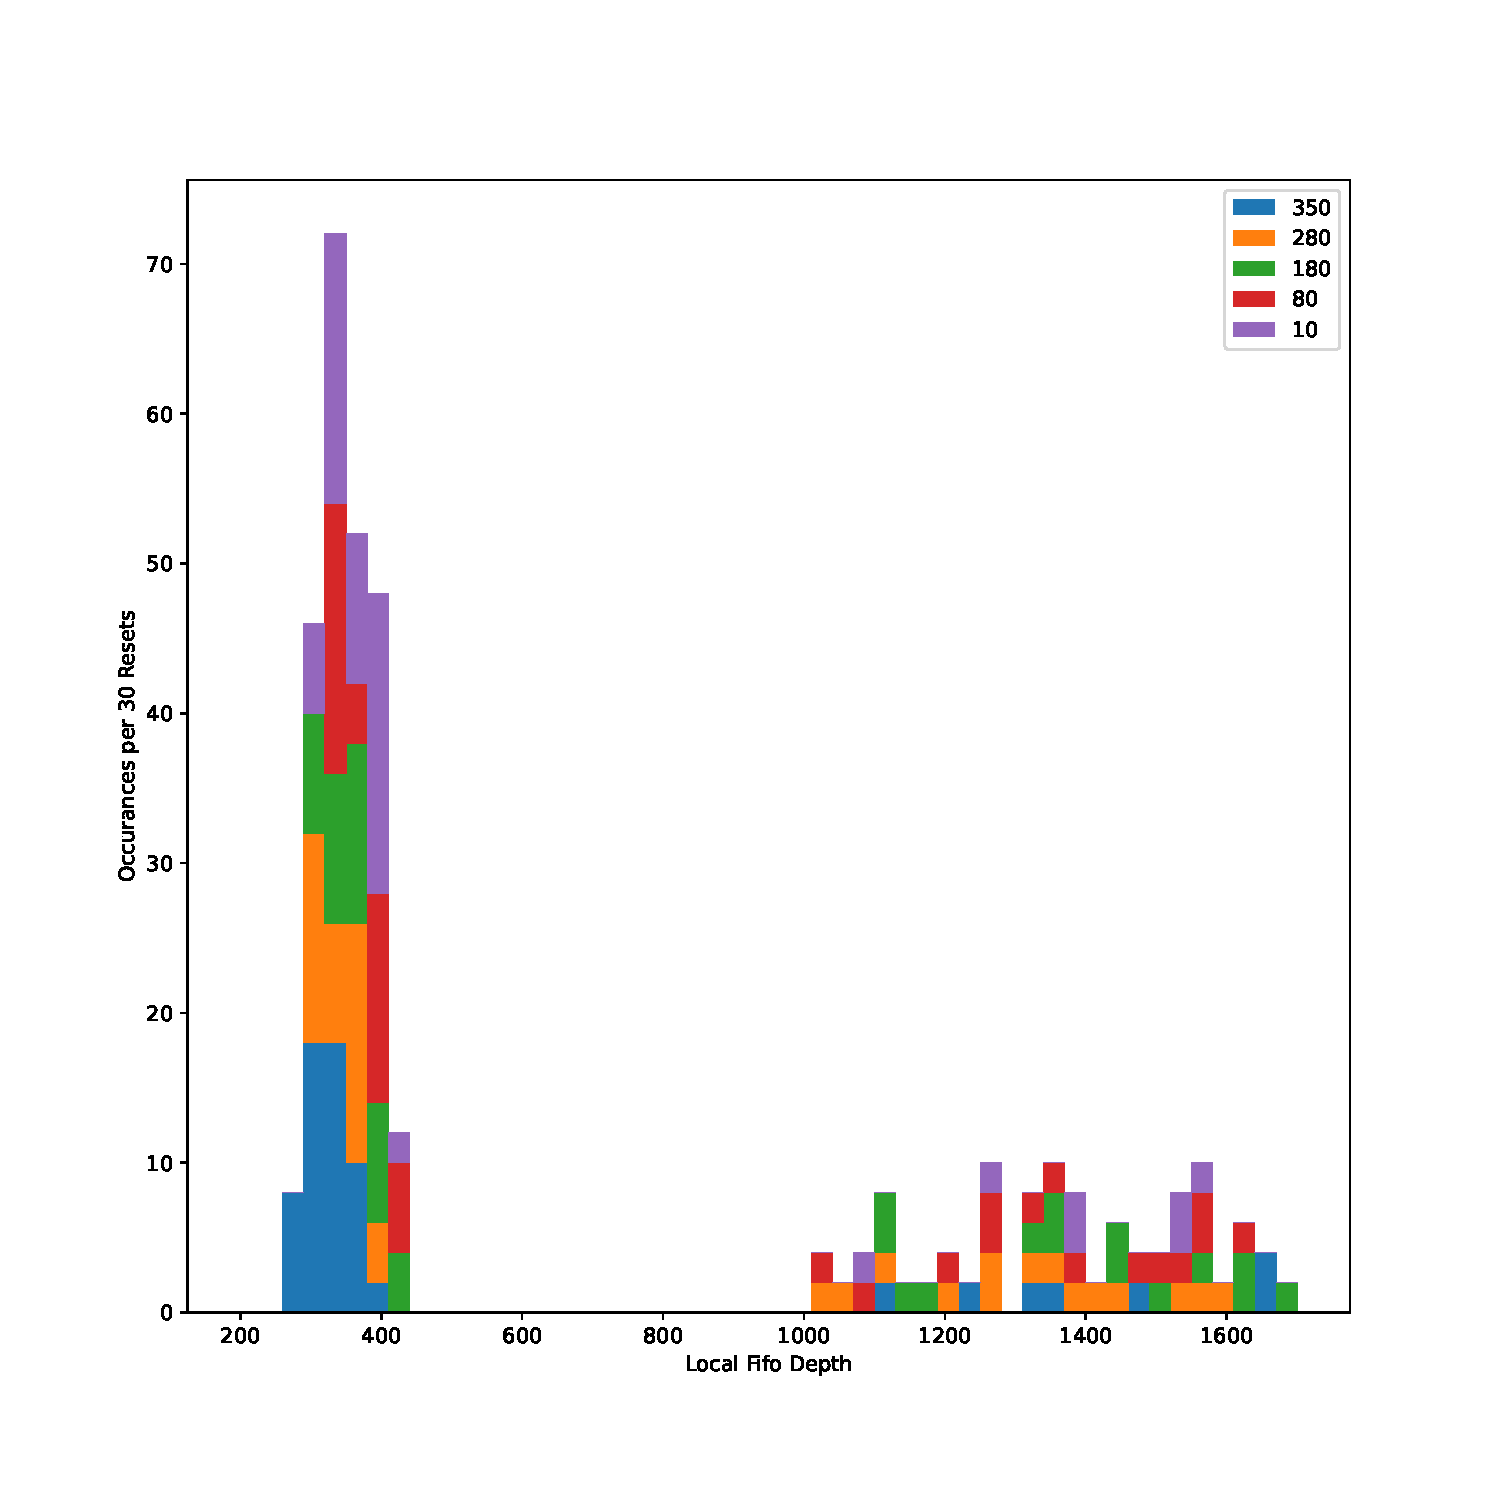
\includegraphics[width=\textwidth]{images/df_zpos_cut.pdf}
  \caption{Colored by Z-position}
\end{subfigure}
\caption{Comparison of Buffer depths as a function of energy for different parameters of $\theta_{z}$ and z-position.
The most important result is shown in Plot-(A), which clearly indicates that only two different parameters account for the distribution of larger local FIFO depths.
As expected, $\theta_{z}$ affects the localization of charge over individual ASICs which affect the local FIFO depth.
Plot-(B) shows the distribution of resets indicated by different z-positions.
Plot-(B) differs in that the second distribution of resets contains elements from each of the different z-positions.
}
\label{fig:compare_integral_zpos_theta}
\end{figure}

\begin{figure}
\centering
\begin{subfigure}{.5\textwidth}
  \centering
  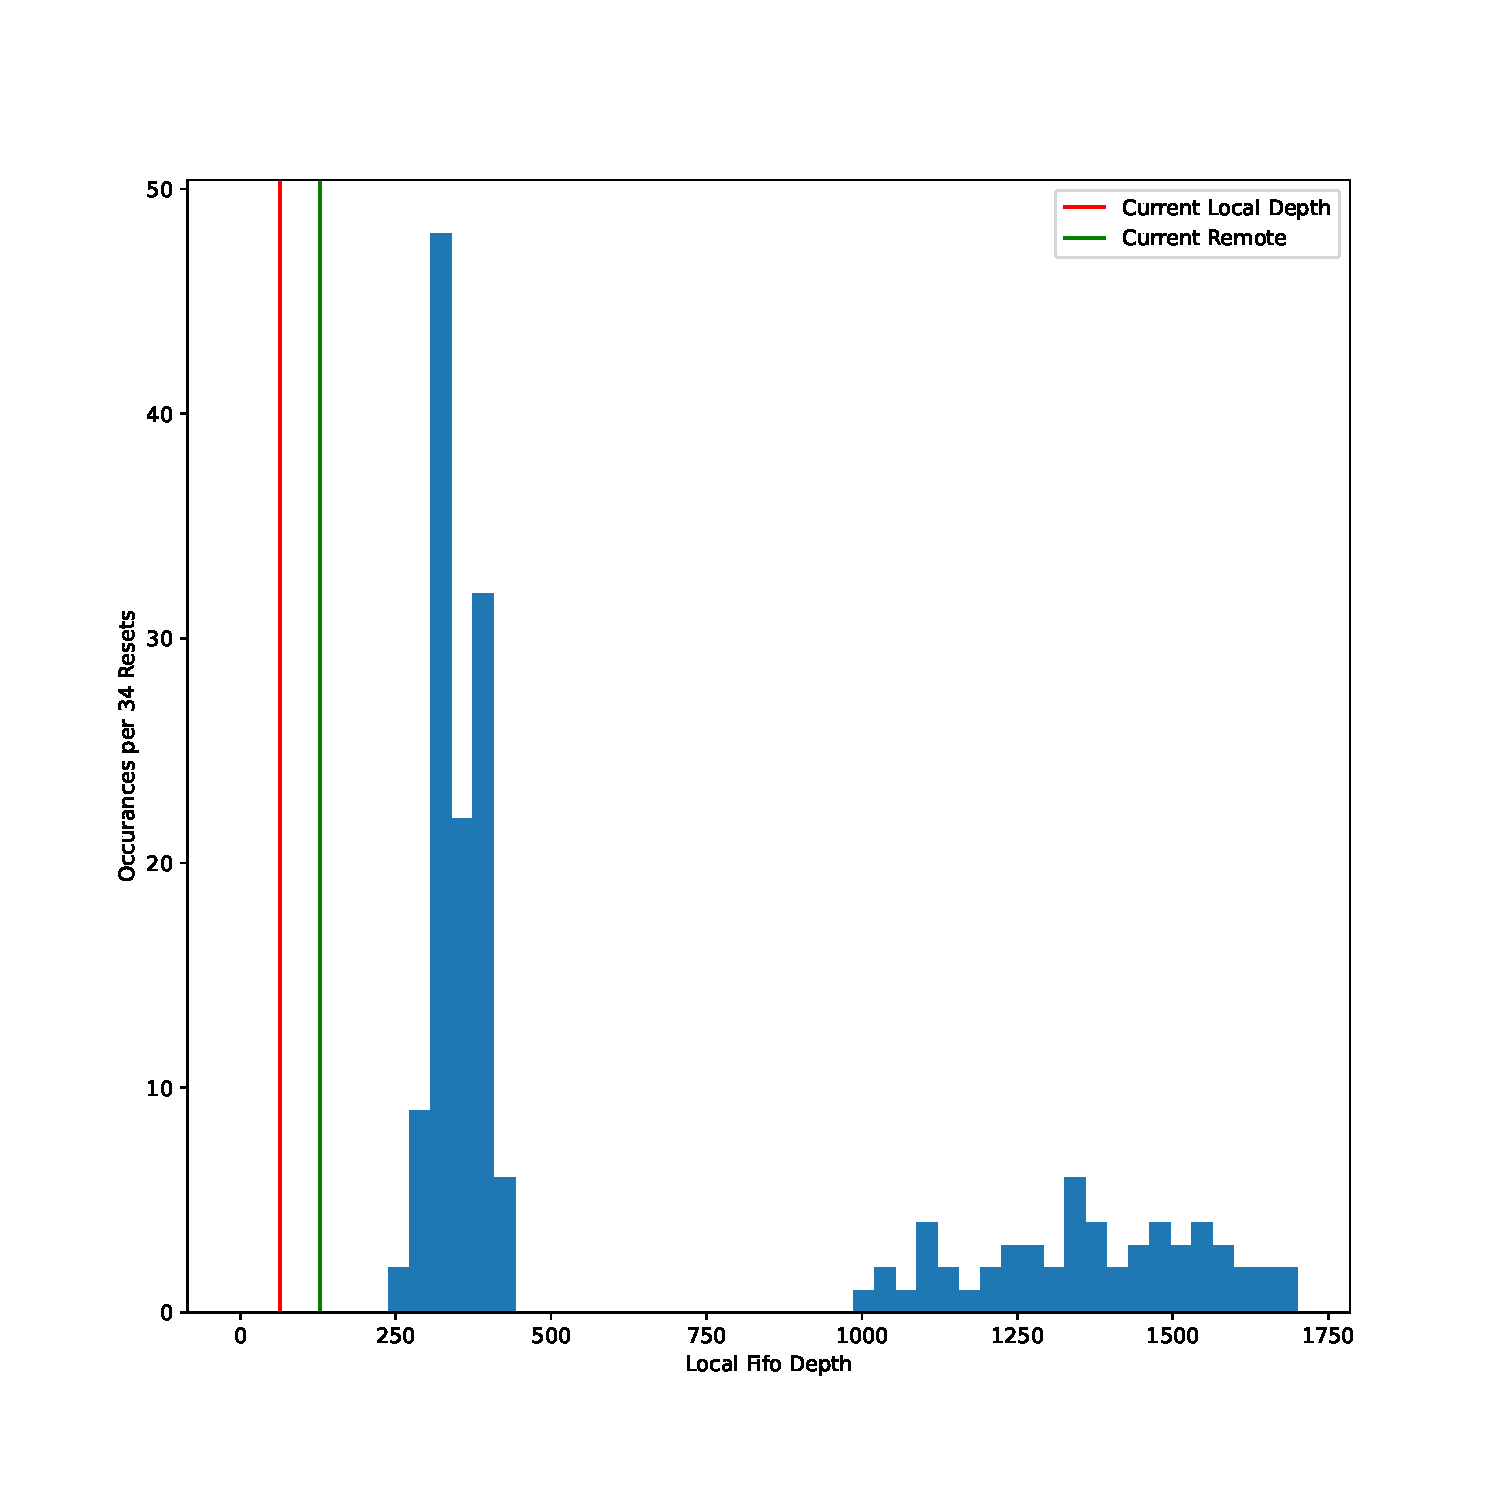
\includegraphics[width=\textwidth]{images/df_nolabel_line.pdf}
  \caption{Comparison of all integrals to current prototype depths.}
\end{subfigure}%
\begin{subfigure}{.5\textwidth}
  \centering
  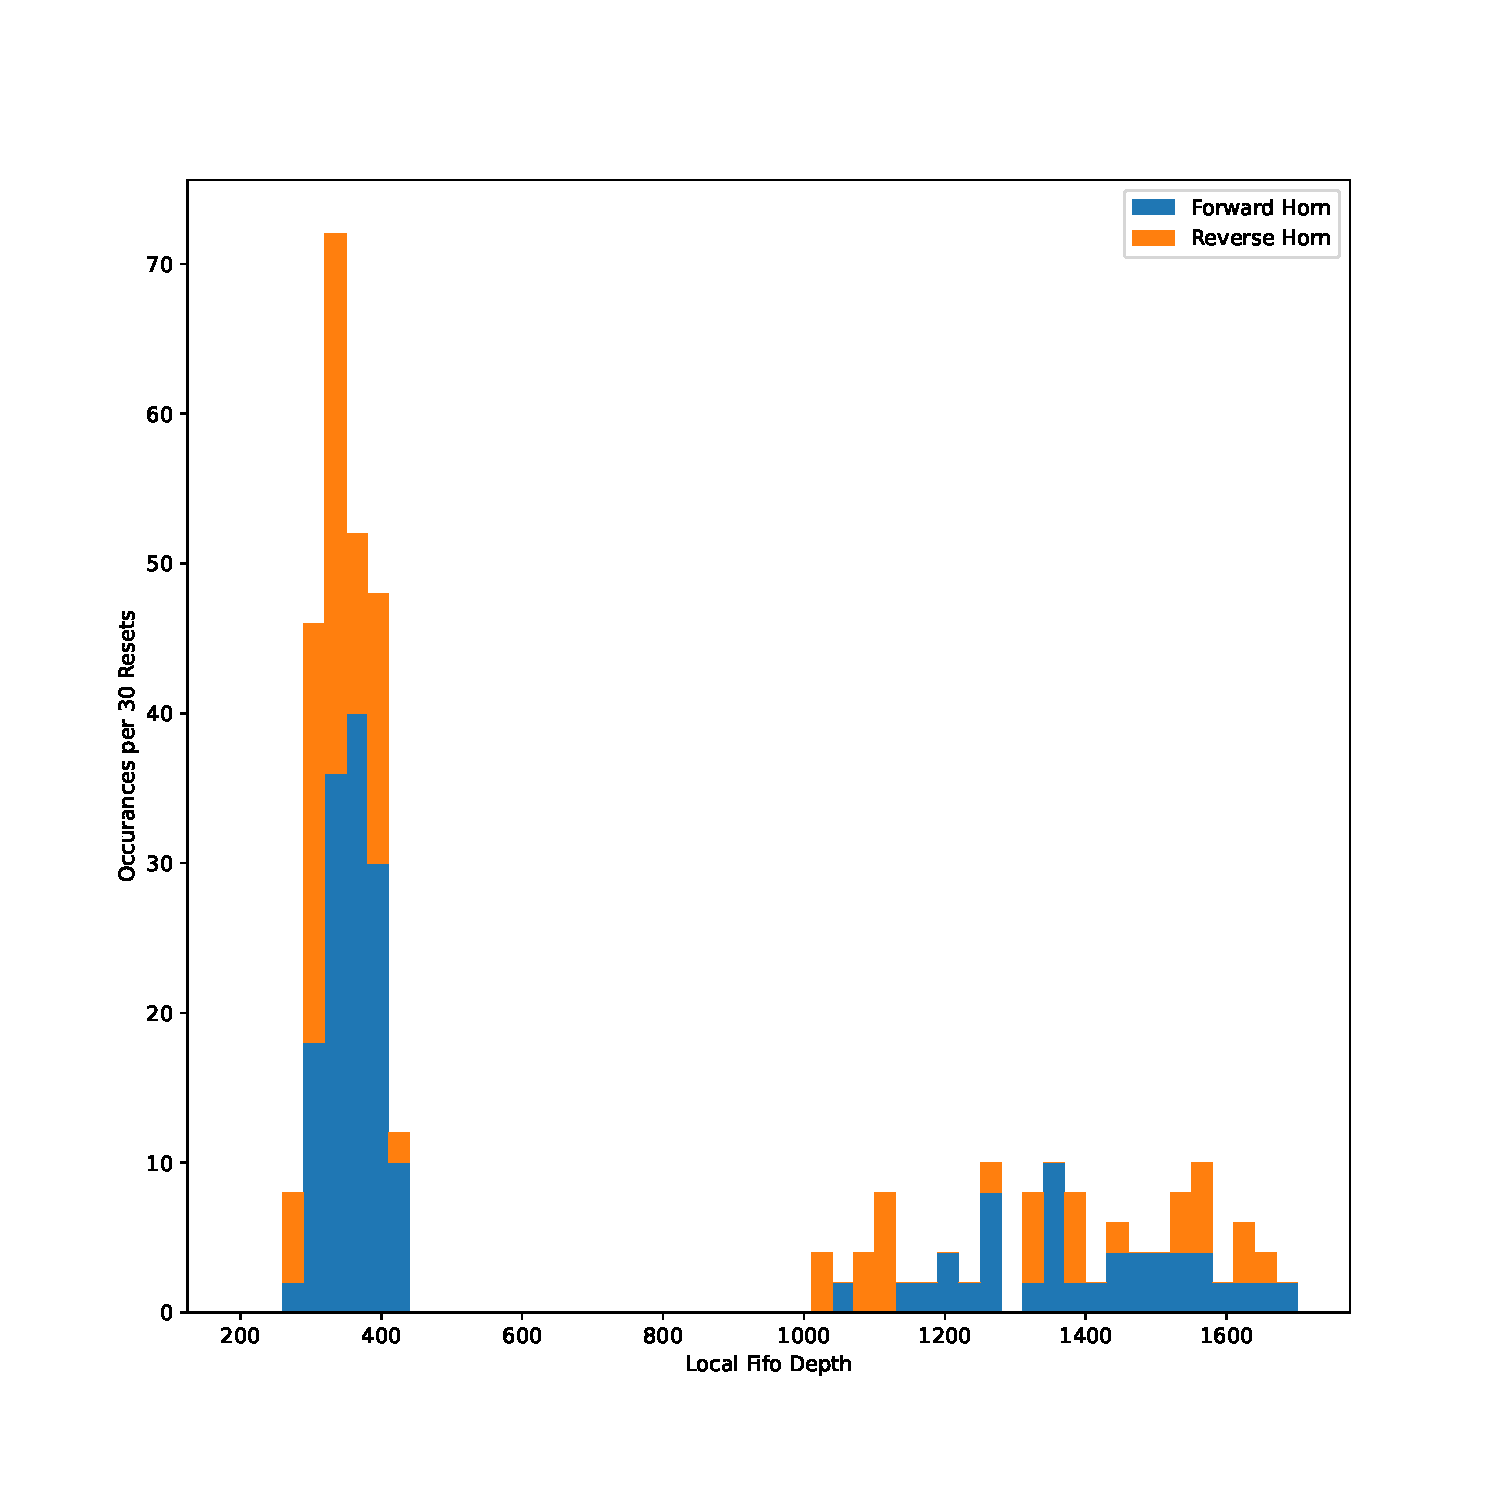
\includegraphics[width=\textwidth]{images/df_horn_cut.pdf}
  \caption{Colored by Z-position}
\end{subfigure}
\caption{Comparison of Buffer depths as in incoming prototype and horn current direction from neutrino beam.}
\label{fig:compare_integral_nolabel}
\end{figure}

The two different distributions indicate that there are at least two different design specifications for future Q-Pix prototypes.
The first capture distribution has a maxmimum value of 426.
Therefore, a Q-Pix ASIC with a local FIFO depth of 426 would be able to fully capture all resets for 99\% of all neutrino interactions under 10~\unit{GeV}.
In order for Q-Pix to measure events of the same energy average energy but with momentum near the azumithal ($\theta_{z} \approx \pm 90$\unit{\degree}) it would require a buffer depth of 1670.

% tie everything together in the final section
\section{Neutrinos, Backgrounds, and Routing}

A valid reconstruction requires all packets to be collected regardless of neutrino type, energy within the valid range, interaction vertex, and should also be able to accept a range of incoming momentum angles.

\subsection{Combining the Digital and Physical Simulations}

%%% Example of Digital Simulation Reconstruction
\begin{figure*}
  \centering
  \begin{subfigure}[b]{0.475\textwidth}
      \centering
      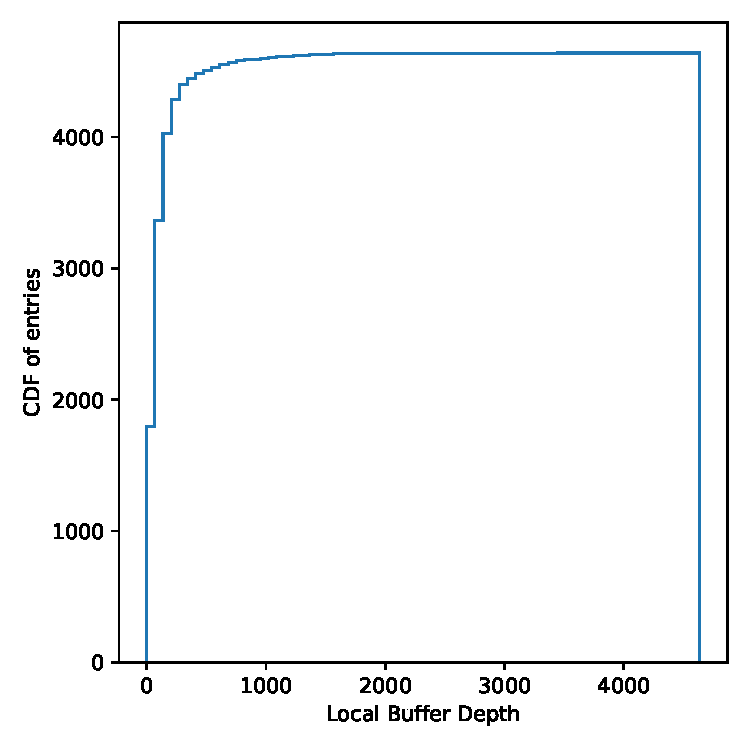
\includegraphics[width=\textwidth]{./images/mp60_16_slow_local_stack.pdf}
      \caption[Network2]%
      {{\small Network 1}}    
  \end{subfigure}
  \hfill
  \begin{subfigure}[b]{0.475\textwidth}  
      \centering 
      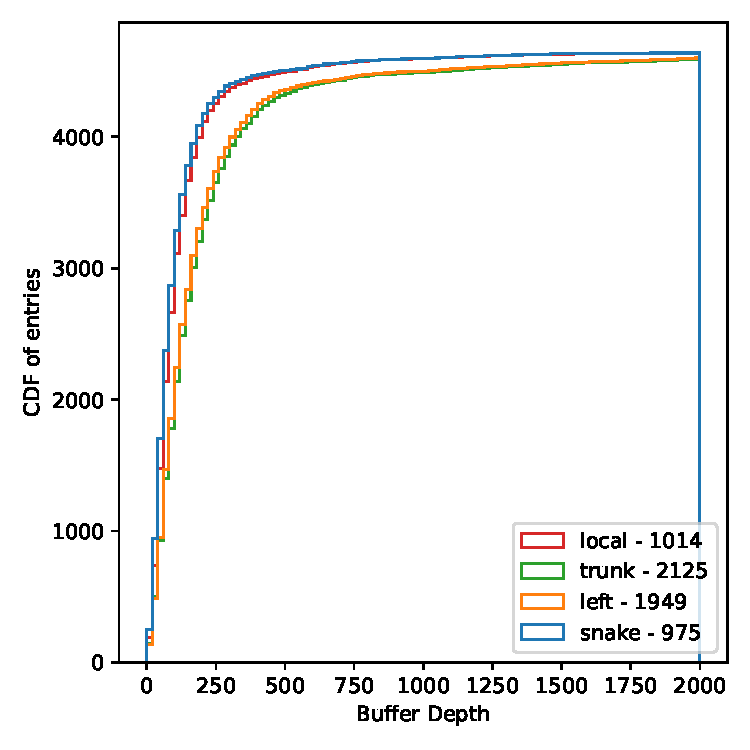
\includegraphics[width=\textwidth]{./images/mp60_16_slow_remote_stack.pdf}
      \caption[]%
      {{\small remote stack}}    
  \end{subfigure}
  \vskip\baselineskip
  \begin{subfigure}[b]{0.475\textwidth}   
      \centering 
      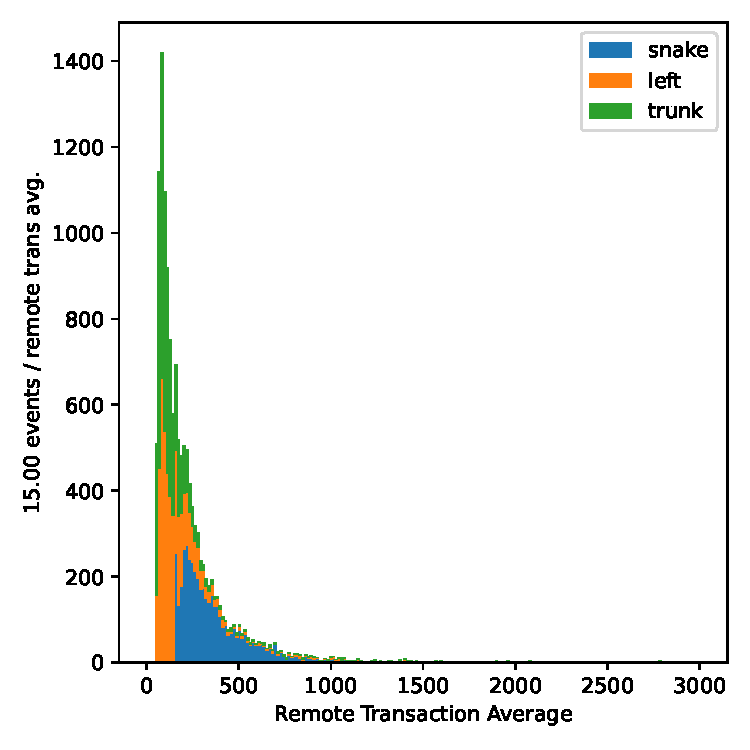
\includegraphics[width=\textwidth]{./images/mp60_16_slow_remote_transactions.pdf}
      \caption[]%
      {{\small transact}}    
  \end{subfigure}
  \hfill
  \begin{subfigure}[b]{0.475\textwidth}   
      \centering 
      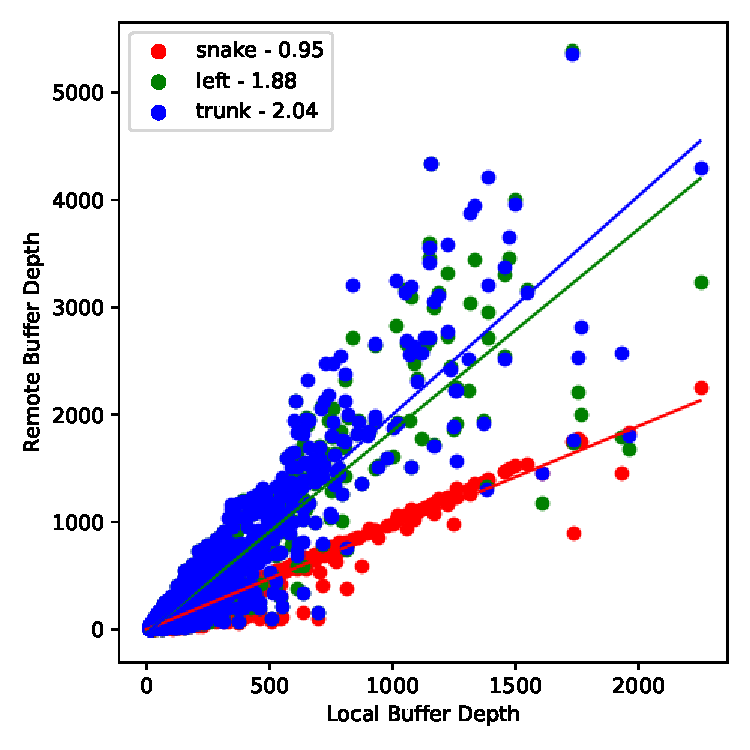
\includegraphics[width=\textwidth]{./images/mp60_16_slow_route_fits.pdf}
      \caption[]%
      {{\small route fits}}    
  \end{subfigure}
  \caption[ Information on the 4 by 4 tile. ]
  {\small all of the data } 
  \label{fig:mp60_fast_plots_for_digital_sim}
\end{figure*}

%%% Example of Digital Simulation Remote Parameterization
\begin{figure*}
  \centering
  \begin{subfigure}[b]{0.475\textwidth}
      \centering
      \includegraphics[width=\textwidth]{./images/mp60_16_slow_route_fits.pdf}
      \caption[]%
      {\small 16 Sized Tile}    
  \end{subfigure}
  \hfill
  \begin{subfigure}[b]{0.475\textwidth}  
      \centering 
      \includegraphics[width=\textwidth]{./images/mp60_64_slow_route_fits.pdf}
      \caption[]%
      {\small 64 Sized tile}    
  \end{subfigure}
  \vskip\baselineskip
  \begin{subfigure}[b]{0.475\textwidth}   
      \centering 
      \includegraphics[width=\textwidth]{./images/mp60_140_slow_route_fits.pdf}
      \caption[]%
      {\small 140 Sized tile}    
  \end{subfigure}
  \hfill
  \begin{subfigure}[b]{0.475\textwidth}   
      \centering 
      \includegraphics[width=\textwidth]{./images/mp60_256_slow_route_fits.pdf}
      \caption[]%
      {\small 256 Sized Tile}    
  \end{subfigure}
  \caption[ Information on the 4 by 4 tile. ]
  {\small all of the data } 
  \label{fig:compare_slow_plots_for_digital_sim_slow}
\end{figure*}


%%% 4x4 Example Digital simulation results
\begin{figure*}
  \centering
  \begin{subfigure}[b]{0.475\textwidth}
      \centering
      \includegraphics[width=\textwidth]{./images/mp60_16_fast_local_stack.pdf}
      \caption[Network2]%
      {{\small Network 1}}    
  \end{subfigure}
  \hfill
  \begin{subfigure}[b]{0.475\textwidth}  
      \centering 
      \includegraphics[width=\textwidth]{./images/mp60_16_fast_remote_stack.pdf}
      \caption[]%
      {{\small remote stack}}    
  \end{subfigure}
  \vskip\baselineskip
  \begin{subfigure}[b]{0.475\textwidth}   
      \centering 
      \includegraphics[width=\textwidth]{./images/mp60_16_fast_remote_transactions.pdf}
      \caption[]%
      {{\small transact}}    
  \end{subfigure}
  \hfill
  \begin{subfigure}[b]{0.475\textwidth}   
      \centering 
      \includegraphics[width=\textwidth]{./images/mp60_16_fast_route_fits.pdf}
      \caption[]%
      {{\small route fits}}    
  \end{subfigure}
  \caption[ Information on the 4 by 4 tile. ]
  {\small example plots for a 4 $\times$ 4 tile. } 
  \label{fig:mp60_plots_for_digital_sim}
\end{figure*}

%%% Example of Digital Simulation Results for 16x16 tile
\begin{figure*}
  \centering
  \begin{subfigure}[b]{0.475\textwidth}
      \centering
      \includegraphics[width=\textwidth]{./images/mp60_16_fast_route_fits.pdf}
      \caption[]%
      {\small 16 Sized Tile}    
  \end{subfigure}
  \hfill
  \begin{subfigure}[b]{0.475\textwidth}  
      \centering 
      \includegraphics[width=\textwidth]{./images/mp60_64_fast_route_fits.pdf}
      \caption[]%
      {\small 64 Sized tile}    
  \end{subfigure}
  \vskip\baselineskip
  \begin{subfigure}[b]{0.475\textwidth}   
      \centering 
      \includegraphics[width=\textwidth]{./images/mp60_140_fast_route_fits.pdf}
      \caption[]%
      {\small 140 Sized tile}    
  \end{subfigure}
  \hfill
  \begin{subfigure}[b]{0.475\textwidth}   
      \centering 
      \includegraphics[width=\textwidth]{./images/mp60_256_fast_route_fits.pdf}
      \caption[]%
      {\small 256 Sized Tile}    
  \end{subfigure}
  \caption[ Information on the 16 by 16 tile. ]
  {\small 16 $\times$ 16 tile of results} 
  \label{fig:compare_fast_plots_for_digital_sim_fast}
\end{figure*}

%% table information
\begin{table}
	\begin{center}
		\begin{tabular}{|c|c|c|c|c|c|}
			\hline
			Freq. & Tile Size & Mean Local Hits & Snake & Left & Trunk \\
			\hline
			5\% & 16 & 48.250 & 423.293 & 166.403 & 138.380 \\
			\hline
			0.5\% & 16 & 51.846 & 449.861 & 177.357 & 147.346 \\
			\hline
			5\% & 64 & 34.129 & 1332.440 & 286.929 & 227.595 \\
			\hline
			0.5\% & 64 & 36.268 & 1400.794 & 301.775 & 239.087 \\
			\hline
			5\% & 140 & 26.521 & 2298.912 & 355.037 & 262.448 \\
			\hline
			0.5\% & 140 & 28.173 & 2416.778 & 373.173 & 275.614 \\
			\hline
			5\% & 256 & 24.343 & 4020.649 & 465.629 & 354.405 \\
			\hline
			0.5\% & 256 & 25.752 & 4209.196 & 487.090 & 370.695 \\
			\hline
		\end{tabular}
	\end{center}
	\caption{Transaction summary data is shown.
	The mean local hits column indicates the mean average of resets injected into the ASICs within the tile from an electron neutrino events.
	The Snake, Left, and Trunk, columns indicate the mean number of remote packet transactions which occured during the full 10 second simulation run.
	As expected, the amount of packet transactions in the snake routing scales with the tile size, whereas the Left and Trunk routings do not.
	The frequency distribution of the tiles does not affect the total number of transactions in the simulated event.
	These results can be used to indicate the amount of power and active time required for a tile to fully readout an electron neutrino event. 
	For example, if a tile size of 256 with a snake routing takes 4020 packets on average to digitize the event, then there are a total of slightly more than one million packets sent.
	If the amount of power used during single packet transaction is known, this ratio could be used to estimate the dissipated power during the back-end readout. 
	}
	\label{tab:transact}
\end{table}

%% table information
\begin{table}
	\begin{center}
		\begin{tabular}{|c|c|c|l|r|l|r|l|r|}
			\hline
			Freq. & Tile Size & Local Hits & 95-S & 99-S & 95-L & 99-L & 95-T & 99-T \\
			\hline
			5\% & 16 & 939 & 320 & 1014 & 535 & 1736 & 607 & 1971 \\
			\hline
			0.5\% & 16 & 1014 & 322 & 975 & 603 & 1949 & 652 & 2125 \\
			\hline
			5\% & 64 & 1200 & 598 & 2191 & 1098 & 4394 & 975 & 4295 \\
			\hline
			0.5\% & 64 & 1307 & 403 & 1328 & 970 & 4298 & 974 & 4521 \\
			\hline
			5\% & 140 & 1182 & 852 & 3486 & 1455 & 6558 & 1343 & 6309 \\
			\hline
			0.5\% & 140 & 1393 & 440 & 1464 & 1327 & 6616 & 1382 & 6757 \\
			\hline
			5\% & 256 & 1456 & 1039 & 3637 & 2026 & 7679 & 2008 & 8250 \\
			\hline
			0.5\% & 256 & 1670 & 527 & 1668 & 1773 & 7460 & 1784 & 7368 \\
			\hline
		\end{tabular}
	\end{center}
	\caption{Buffer Data}
	\label{tab:buffers}
\end{table}

%% table information
\begin{table}
	\begin{center}
		\begin{tabular}{|c c|c|c|c|c|}
			\hline
			Tile Size & Frequency & Snake & Left & Trunk & Push \\
			\hline
			16 & 0.5\% & 0.948 & 1.879 & 2.039 & 0.979 \\
			& 5\% & 1.041 & 1.823 & 2.082 & 1.031 \\
			\hline
			64 & 0.5\% & 1.006 & 2.514 & 2.727 & 0.999 \\
			& 5\% & 1.623 & 3.176 & 2.969 & 1.11 \\
			\hline
			140 & 0.5\% & 1.021 & 3.033 & 3.131 & na \\
			& 5\% & 1.966 & 3.506 & 3.481 & na \\
			\hline
			256 & 0.5\% & 1.027 & 3.243 & 3.336 & na \\
			& 5\% & 1.981 & 3.616 & 3.913 & na \\
			\hline
		\end{tabular}
	\end{center}
	\caption{Transaction fit summary results.
	The values shown from the fits indicate the linear fit to the results to predict the relationship between the local and remote FIFO depth requirements.
	Push fit data is not available for larger tiles (140 and 256) due to simulation time constraints.
	}
	\label{tab:fit}
\end{table}

\section{Summary and Further Studies}~\label{sec:further_studies}
